\documentclass[12pt, a4paper]{report}

\usepackage[spanish]{babel}   % Para el idioma
\usepackage{amssymb,amsfonts,amsmath,latexsym}   % Para las fuentes, simbolos matematicos ect
\usepackage{csquotes}
\usepackage[style=apa, backend=biber]{biblatex}
%\usepackage[]{natbib}
\addbibresource{bibliografia.bib}

%\usepackage{cite}          % Para citar bibliografia
%\usepackage[backref=page]{hyperref} % Para referenciar
\usepackage{hyperref}     % Para referenciar
\usepackage{graphicx}     % Para incluir graficos
\usepackage{fancyhdr}     % Para los encabezados
\usepackage{xcolor}      % Para definir colores
\usepackage{setspace}    % Para incluir interlineados
\usepackage{booktabs}    % Para hacer tablas
\usepackage{longtable}   % Para el tipo de tablas utilizados
\usepackage{textcomp}    % Para algunos signos y simbolos
\usepackage{makeidx}     % Para hacer el indice alfabetico
\usepackage{bm}         % Para escribir simbología en negrita
\usepackage{pdfpages}    % Para incluir un pdf en el escrito
\usepackage[T1]{fontenc}
\usepackage{mathptmx}

%%%%%%%%%%%%%%%%%%%%% DEFINICION DE LA HOJA %%%%%%%%%%%%%%%%%%%%%%%%%%%

\pagestyle{headings}  % Encabezados
% \topmargin 0cm
% \oddsidemargin 0.7cm   
% \textheight 21cm
% \textwidth 15cm
\parindent 0cm
\parskip 0.2cm
\usepackage[top=3.5cm, bottom=3cm, left=3cm, right=2.5cm]{geometry}


\def \ds{\displaystyle}
\def\sqr#1#2{{\vcenter{\vbox{\hrule height.#2pt\hbox{\vrule width.#2pt height#1pt \kern#1pt \vrule width.#2pt} \hrule height.#2pt}}}}
\def\square{\mathchoice\sqr34\sqr34\sqr{2.1}3\sqr{1.5}3}

\setcounter{secnumdepth}{3}

%%%%%%%%%%%%%%%%%%%%%%%%%%%%%%%%%%%%%%%%%%%%%%%%%%%%%%%%%%%%%%%%%%%%%%%%%%%%%

% -------------------- Letras Especiales -------------------------

\def \N{\mathbb{N}}
\def \Z{\mathbb{Z}}
\def \Q{\mathbb{Q}}
\def \R{\mathbb{R}}
\def \C{\mathbb{C}}
\def \ds{\displaystyle}

\newcommand{\argmin}{\mathop{\mathrm{argmin}}\limits}
\newcommand{\minimo}{\mathop{\mathrm{min}}\limits}
\newcommand{\maximo}{\mathop{\mathrm{max}}\limits}

% -------------------- Environment delimiters --------------------

\newtheorem{defn}{Definici\'on}[chapter]
\newtheorem{lem}[defn]{Lema}
\newtheorem{prop}[defn]{Proposici\'on}
\newtheorem{theorem}[defn]{Teorema}
\newtheorem{cor}[defn]{Corolario}
\newtheorem{rem}[defn]{Observaci\'on}
\newtheorem{exmpl}[defn]{Ejemplo}

\DeclareUnicodeCharacter{0301}{\'{e}}
% \newenvironment{undef}[1]
%    {\vspace{3.3mm}\noindent{\bf #1}\it}
%    {\vspace{3.3mm}}

\newenvironment{proof}[1]
   {\trivlist \item[\hskip \labelsep{\it #1}]}
   {\hfill\mbox{$\square$}
   \endtrivlist}

% -------------------- Mi Tesis --------------------

\setlength{\headheight}{0.5cm}
\rhead{\begin{picture}(0,0) \put(-99.7,0){\includegraphics[width=40mm]{0_1_Caratula/austral_logo.jpg}} \end{picture}} % Encabezado
\renewcommand{\headrulewidth}{0.5pt}
\pagestyle{fancy} %Estilo de pagina

\renewcommand{\baselinestretch}{1.5
} % interlineado 1.5

\makeindex % para que cree el índice alfabetico 

\begin{document}
%
\renewcommand{\listfigurename}{\'Indice de Figuras} % Para que titule con inicial en mayuscula
%
\renewcommand{\listtablename}{\'Indice de Cuadros}  % Para que titule con inicial en mayuscula
%
\renewcommand{\indexname}{\'Indice Alfab\'etico} % Para que titule con inicial en mayuscula
%
\pagenumbering{Roman} % Inicia pagimación en números Romanos 
%
%\includepdf[pages=1-12]{Portada_y_Formulario_E.pdf}   % Para incluir la portada y el formulario E
%
%\addcontentsline{toc}{chapter}{Portada y Formulario E}  % Agrega el formulario al indice general
%
%
% TESIS DE DOCTORADO - GUILLERMO FEDERICO UMBRICHT


\thispagestyle{empty}

\begin {center}
%\textbf{UNIVERSIDAD AUSTRAL}

\includegraphics[trim = 1250mm 0mm 0mm 0mm, clip, width=0.28\textwidth]{0_1_Caratula/austral_logo.jpg}

\vspace{0.5cm}
\LARGE\textbf{UNIVERSIDAD AUSTRAL}
\break
%\textbf{FACULTAD DE CIENCIAS EMPRESARIALES}
\large Facultad de Ciencias Empresariales

\vspace{1.cm}
%\textbf{\large Modelo matemático de variables empíricas en consumo
%intertemporal con preferencias inconsistentes}

\large Modelo de consumo intertemporal en tiempo continuo con preferencias inconsistentes y descuento cuasi-hiperbólico.
% DESCUENTO CUASI-HIPERBÓLICO EN MODELO DE CONSUMO INTERTEMPORAL 

\vspace{1.cm}
% \textbf{\large Tesina para licenciatura en Economía empresarial}
\LARGE TESIS \break
\large  Licenciatura en Economía empresarial

\vspace{0.5cm}

\normalsize PRESENTA: \break
\large Francisco Sesto
% \textbf{Francisco Sesto}

\vspace{0.5cm}

% \textbf{Director}
\normalsize DIRECTOR: \break
\large Guillermo Federico Umbricht

\vspace{2cm}
Octubre de 2023
\end {center}


% \vspace{1.5cm}


% \noindent \textbf{Director: Guillermo Federico Umbricht}
% \noindent Director: Guillermo Federico Umbricht


% \vspace{1.0cm}


% \rightline{Octubre de 2023}


% Diseño viejo
% \thispagestyle{empty}


% \begin {center}

% \includegraphics[scale=.05]{0_1_Caratula/austral_logo.jpg}

% \medskip

% \textbf{UNIVERSIDAD AUSTRAL}

% \smallskip

% \textbf{Facultad de Ciencias económicas}

% \smallskip



% \vspace{1.0cm}


% \textbf{\large Tesina de grado de Economía empresarial}


% \vspace{1.5cm}


% \textbf{\large Modelo matemático de variables empíricas en consumo
% intertemporal con preferencias inconsistentes}


% \vspace{1.5cm}


% \textbf{Francisco Sesto}

% \end {center}


% \vspace{1.5cm}


% \noindent \textbf{Director: Guillermo Federico Umbricht}



% \vspace{2.0cm}


% \rightline{Octubre de 2023}  %%%%%%% Carátula
%
\thispagestyle{empty}  % No la enumera
%
\newpage % Deja una hoja en blanco
$\ $
%
\thispagestyle{empty}  % No la enumera
%
% \chapter*{}
\begin{flushright}
\textit{Dedicado a todos los que  \\
  creyeron que era posible}
\end{flushright}
  %%%%%%% Dedicatoria
% %
% \newpage % Deja una hoja en blanco
% $\ $
% \thispagestyle{empty}  % No la enumera
% %
% \chapter*{Agradecimientos}
\markright{AGRADECIMIENTOS}

Haber realizado un trabajo como \'este es producto del esfuerzo de muchas
personas durante muchos a\~nos. Quiero aprovechar esta ocasi\'on para expresarles
mis m\'as sinceros agradecimientos.

Quiero agradecer especialmente a:

Mi directora, la doctora Diana Rubio, por el aporte significativo a mi
formaci\'on durante los \'ultimos a\~nos y por la colaboraci\'on impartida para la
realizaci\'on de este trabajo. Sin su incondicional apoyo no lo hubiese podido hacer.

Mi co-director, el doctor Claudio El Hasi, por las diligentes conversaciones tenidas 
durante el proceso de trabajo sobre diferentes tem\'aticas.

A mi consejero de estudios y amigo, el Doctor Rodolfo Echarri, por estar
siempre predispuesto a escuchar y colaborar con cualquier inquietud, por el
tiempo que me ha dedicado y por sentarse a pensar conmigo durante horas
cualquier idea loca que se me ocurra.

Al Doctor Domingo Tarzia, por los valiosos y productivos d\'ias enteros de 
trabajo compartido.

A la Doctora Mabel Rodriguez, por creer en m\'i, por brindarme su apoyo y su confianza.


A Natalia Engelhardt, por leer minusiosamente esta tesis, realizar 
correcciones y sugerencias.  

A mis amigos, Diego, Hern\'an, Lugo, Juan Pablo, el colo, por estar siempre, por creer en m\'i 
y por acompa\~narme en este proceso. 

A muchas otras personas que de una u otra manera han aportado para que
pueda llegar a esta instancia, Anita, Luis, Marisol, Norma, Eva, Cristina, Adriana,
Olga, Gabriel, Ceci.
  %%%%%%% Agradecimientos
% %
% \singlespace     % interlineado simple para el indice, las figuras y las tablas
% %
\tableofcontents  %%%%%%% Índice
% %
% \addcontentsline{toc}{chapter}{\'Indice General}  % Agrega la lista al indice general
% %
% \newpage % Deja una hoja en blanco
% $\ $
% %
% \thispagestyle{empty}  % No la enumera
% %
% \listoffigures    %%%%%%% Índice de figuras
% %
% \addcontentsline{toc}{chapter}{\'Indice de Figuras} % Agrega la lista al indice general 
% %
% \listoftables     %%%%%%% Índice de tablas
% %
% \addcontentsline{toc}{chapter}{\'Indice de Cuadros} % Agrega la lista al indice general 
% %
% \spacing{1.5}       %interlineado 1.5 para el resto.
% %
% \chapter*{Nomenclatura}
\addcontentsline{toc}{chapter}{Nomenclatura}
\markright{NOMENCLATURA}

\begin{longtable}{p{5mm} c p{120mm} }
%
\multicolumn{3}{l}{\textbf{May\'usculas} }\\
\\
$A$ & --- & Connjunto admisible de toma de datos.\\
$Ag$ & --- & S\'imbolo qu\'imico de la Plata.\\
$Al$ & --- & S\'imbolo qu\'imico del Aluminio.\\
$Cu$ & --- & S\'imbolo qu\'imico del Cobre.\\
$E_e$ & --- & Elasticidad exacta.\\
$E_m$ & --- & Elasticidad m\'inima.\\
$E_M$ & --- & Elasticidad m\'axima.\\
$E_{u}^{h}$ & --- & Elasticidad de $u$ con respecto a $h$.\\
$E_{l}^{q}$ & --- & Elasticidad de $l$ con respecto a $q$.\\
$F$ & --- & Fuente puntual $\textbf{[{$^{\circ}$}C]}$.\\
$Fe$ & --- & S\'imbolo qu\'imico del Hierro.\\
$F_{flot}$ & --- & Fuerza de flotabilidad $\textbf{[N]}$.\\
$F_N$ & --- & Fuerza neta vertical sobre el cuerpo $\textbf{[N]}$.\\
$G_r$ & --- & N\'umero adimensional de Grashof.\\
$J$ & --- & Funcional de minimizaci\'on.\\
$L$ & --- & Longitud de la barra $\textbf{[m]}$.\\
$Ni$ & --- & S\'imbolo qu\'imico del Niquel.\\
$N_u$ & --- & N\'umero adimensional de Nusselt.\\
$P$ & --- & Peso del cuerpo $\textbf{[N]}$.\\
$Pb$ & --- & S\'imbolo qu\'imico del Plomo.\\
$P_r$ & --- & N\'umero adimensional de Prandtl.\\
$Q$ & --- & Flujo t\'ermico en el \'ultimo elemento de la barra $\textbf{[W/m{$^{2}$}]}$.\\
$Q_1$ & --- & Flujo t\'ermico entrante a un elemento de la barra $\textbf{[W/m{$^{2}$}]}$.\\
$Q_2$ & --- & Flujo t\'ermico que permanece en un elemento de la barra $\textbf{[W/m{$^{2}$}]}$.\\
$Q_3$ & --- & Flujo t\'ermico saliente de un elemento de la barra $\textbf{[W/m{$^{2}$}]}$.\\
$Q_f$ & --- & Flujo t\'ermico en el fluido $\textbf{[W/m{$^{2}$}]}$.\\
$R_a$ & --- & N\'umero adimensional de Rayleigh.\\
$R_\mu$ & --- & Operador de regularizaci\'on.\\
$S$ & --- & \'Area transversal de un elemento infinitesimal de la barra $\textbf{[m{$^{2}$}]}$.\\
$S_{D}^{p_i}$ & --- & Sensibilidad de $D$ con respecto al par\'ametro $p_i$.\\
$S_{u}^{\alpha^2}$ & --- & Sensibilidad de $u$ con respecto a $\alpha^2$ $\textbf{[({$^{\circ}$}C s{$^{2}$})/m]}$.\\
$S_M$ & --- & Sensibilidad m\'axima $\textbf{[({$^{\circ}$}C s{$^{2}$})/m]}$.\\
$Sn$ & --- & S\'imbolo qu\'imico del Esta\~no.\\
$T_a$ & --- & Temperatura ambiente $\textbf{[{$^{\circ}$}C]}$.\\
$V_c$ & --- & Volumen del cuerpo $\textbf{[m{$^{3}$}]}$.\\
%
\\
\multicolumn{3}{l}{\textbf{Min\'usculas} }\\
\\
$c_p$ & --- & Calor espec\'ifico $\textbf{[J/kg {$^{\circ}$}C]}$.\\
$c_{p_f}$ & --- & Calor espec\'ifico del fluido $\textbf{[J/kg {$^{\circ}$}C]}$.\\
$d$ & --- & Di\'ametro de la barra $\textbf{[m]}$.\\
$f$    & --- & Fuente $\textbf{[{$^{\circ}$}C]}$.\\
$\tilde{f}$    & --- & Fuente $\textbf{[{$^{\circ}$}C]}$.\\
$f_n$    & --- & Desarrollo en serie de la fuente $\textbf{[{$^{\circ}$}C]}$.\\
$f_\delta$    & --- & Fuente ruidosa $\textbf{[{$^{\circ}$}C]}$.\\
$f_{\delta,\mu}$    & --- & Fuente regularizada $\textbf{[{$^{\circ}$}C]}$.\\
$g$     & --- & Aceleraci\'on gravitacional $\textbf{[m/s{$^{2}$}]}$.\\
$h$     & --- & Coeficiente de pel\'icula $\textbf{[W/(m{$^{2}$}{$^{\circ}$}C)]}$.\\
$l$ & --- & Posici\'on de interfaz $\textbf{[m]}$.\\
$l_\epsilon$ & --- & Aproximaci\'on de la posici\'on de interfaz $\textbf{[m]}$.\\
$q$ & --- & Flujo t\'ermico $\textbf{[W/m{$^{2}$}]}$.\\
$q_\epsilon$ & --- & Flujo t\'ermico ruidoso $\textbf{[W/m{$^{2}$}]}$.\\
$q_m$ & --- & Flujo t\'ermico m\'inimo $\textbf{[W/m{$^{2}$}]}$.\\
$q_M$ & --- & Flujo t\'ermico m\'aximo $\textbf{[W/m{$^{2}$}]}$.\\
$q_p$ & --- & Flujo t\'ermico promedio $\textbf{[W/m{$^{2}$}]}$.\\
$\dot{q}_{cond}$ & --- & Flujo t\'ermico conductivo $\textbf{[W/m{$^{2}$}]}$.\\
$\dot{q}_{conv}$ & --- & Flujo t\'ermico convectivo $\textbf{[W/m{$^{2}$}]}$.\\
$t$     & --- & Variable temporal $\textbf{[s]}$.\\
$t_j$     & --- & Instante de tiempo particular $\textbf{[s]}$.\\
$t_0$     & --- & Tiempo de toma de mediciones $\textbf{[s]}$.\\
$t_\infty$     & --- & Tiempo relativo al estado estacionario $\textbf{[s]}$.\\
$u$    & --- & Temperatura de la barra $\textbf{[{$^{\circ}$}C]}$.\\
$u_e$    & --- & Temperatura en estado estacionario $\textbf{[{$^{\circ}$}C]}$.\\
$u_{\epsilon}$    & --- & Medici\'on de temperatura $\textbf{[{$^{\circ}$}C]}$.\\
$u_s$    & --- & Temperatura en la superficie $\textbf{[{$^{\circ}$}C]}$.\\
$u_0$    & --- & Temperatura externa a la barra $\textbf{[{$^{\circ}$}C]}$.\\
$u_{\infty}$    & --- & Temperatura lejos de la superficie $\textbf{[{$^{\circ}$}C]}$.\\
$v$    & --- & Temperatura de la barra (funci\'on auxiliar) $\textbf{[{$^{\circ}$}C]}$.\\
$w$    & --- & Temperatura de la barra (funci\'on auxiliar) $\textbf{[{$^{\circ}$}C]}$.\\
$x$     & --- & Variable espacial $\textbf{[m]}$.\\
$\bm x$     & --- & Vector de toma de datos.\\
$x_i$     & --- & Posici\'on particular sobre la barra $\textbf{[m]}$.\\
$y$    & --- & Mediciones de temperatura $\textbf{[{$^{\circ}$}C]}$.\\
$y_\delta$    & --- & Mediciones ruidosas de temperatura $\textbf{[{$^{\circ}$}C]}$.\\
%
\\
\multicolumn{3}{l}{\textbf{Letras Griegas} }\\
\\
$\alpha^2$ & --- & Coeficiente de difusividad t\'ermica $\textbf{[m{$^{2}$}/s]}$.\\
$\hat{\alpha^2}$ & --- & Coeficiente de difusividad t\'ermica estimado $\textbf{[m{$^{2}$}/s]}$.\\
$\alpha_{A}^{2}$ & --- & Coeficiente de difusividad t\'ermica del material $A$ $\textbf{[m{$^{2}$}/s]}$.\\
$\alpha_{B}^{2}$ & --- & Coeficiente de difusividad t\'ermica del material $B$ $\textbf{[m{$^{2}$}/s]}$.\\
$\alpha_{M}^{2}$ & --- & Coeficiente de difusividad t\'ermica del material $\textbf{[m{$^{2}$}/s]}$.\\
$\beta$ & --- & Velocidad del fluido $\textbf{[m/s]}$.\\
$\beta_V$ & --- & Coeficiente de expanci\'on volum\'etrica $\textbf{[1/K]}$.\\
$\delta$     & --- & Espesor de la capa l\'imite t\'ermica $\textbf{[m]}$.\\
$\delta_M$     & --- & Ruido m\'aximo.\\
$\Delta x$     & --- & Paso espacial de discretizaci\'on $\textbf{[m]}$.\\
$\Delta t$     & --- & Paso temporal de discretizaci\'on $\textbf{[s]}$.\\
$\Delta u$     & --- & Variaci\'on de temperatura  $\textbf{[{$^{\circ}$}C]}$.\\
$\Delta E$     & --- & Variaci\'on de elasticidad .\\
$\overline{\Delta u_c}$   & --- & Variaci\'on de temperatura media en el cuerpo $\textbf{[{$^{\circ}$}C]}$.\\
$\overline{\Delta u_f}$   & --- & Variaci\'on de temperatura media en el fluido $\textbf{[{$^{\circ}$}C]}$.\\
$\epsilon$ & --- & Cota para el error de medici\'on.\\
$\epsilon_i$ & --- & Ruido simulado.\\
$\varphi$    & --- & Temperatura de la barra (funci\'on auxiliar) $\textbf{[{$^{\circ}$}C]}$.\\
$\kappa$ & --- & Coeficiente de conductividad t\'ermica $\textbf{[W/m {$^{\circ}$}C]}$.\\
$\kappa_A$ & --- & Coeficiente de conductividad t\'ermica del material $A$ $\textbf{[W/m {$^{\circ}$}C]}$.\\
$\kappa_B$ & --- & Coeficiente de conductividad t\'ermica del material $B$ $\textbf{[W/m {$^{\circ}$}C]}$.\\
$\kappa_C$ & --- & Coeficiente de conductividad t\'ermica del cuerpo $\textbf{[W/m {$^{\circ}$}C]}$.\\
$\kappa_f$ & --- & Coeficiente de conductividad t\'ermica del fluido $\textbf{[W/m {$^{\circ}$}C]}$.\\
$\kappa_m$ & --- & Coeficiente de conductividad t\'ermica m\'inimo $\textbf{[W/m {$^{\circ}$}C]}$.\\
$\kappa_M$ & --- & Coeficiente de conductividad t\'ermica m\'aximo $\textbf{[W/m {$^{\circ}$}C]}$.\\
$\nu$ & --- & Ritmo de intercambio de calor por flujo lateral $\textbf{[1/s]}$.\\
$\nu_c$ & --- & Viscocidad cinem\'atica del fluido $\textbf{[m$^{2}$/s]}$.\\
$\mu_d$ & --- & Viscocidad din\'amica del fluido $\textbf{[kg/m\,s]}$.\\
$\mu^2$     & --- & Par\'ametro de regularizaci\'on.\\
$\Theta$     & --- & Conjunto admisible de soluciones.\\
$\bm \theta$     & --- & Vector de par\'ametros desconocidos.\\
$\rho$ & --- & Densidad $\textbf{[kg/m{$^{3}$}]}$.\\
$\rho_c$ & --- & Densidad del cuerpo $\textbf{[kg/m{$^{3}$}]}$.\\
$\rho_f$ & --- & Densidad del fluido $\textbf{[kg/m{$^{3}$}]}$.\\
$\rho_{\infty}$ & --- & Densidad del fluido lejos de la superficie del cuerpo $\textbf{[kg/m{$^{3}$}]}$.\\
$\sigma^2$     & --- & Varianza.\\
$\tau_1$     & --- & Par\'ametro de estabilidad.\\
$\tau_2$     & --- & Par\'ametro de estabilidad.\\
$\tau_3$     & --- & Par\'ametro de estabilidad.\\

\end{longtable}


 % Nomenclatura
% %
\newpage % Deja una hoja en blanco
 $\ $
\thispagestyle{empty}  % No la enumera
% %
 \chapter*{Resumen}
\addcontentsline{toc}{chapter}{Resumen}
\markright{RESUMEN}


Esta tesis se centra en la investigación y en el desarrollo de una mejora del modelo propuesto por \textcite{feigenbaum2021deviation} en el ámbito del consumo intertemporal. El objetivo principal de este estudio es incorporar una nueva función de descuento en el modelo existente y representar de manera más precisa la percepción de los individuos en el proceso de toma de decisiones relacionado con el consumo a lo largo del tiempo.
Este trabajo se enfoca en los siguientes aspectos clave:

\begin{itemize}
\item \textit{\textbf{Formulación del modelo:}} Se han completado los cálculos inconclusos y se han proporcionado comentarios relevantes sobre los resultados del modelo de consumo intertemporal en tiempo continuo que considera preferencias inconsistentes propuesto por \textcite{feigenbaum2021deviation}. 


\item \textit{\textbf{Función de descuento cuasi-hiperbólica:}} En este trabajo, se ha incorporado al modelo de \textcite{feigenbaum2021deviation}, una función de descuento cuasi-hiperbólica introducida en \parencite{myerson1995discounting}, la cual, respaldada por evidencia empírica, proporciona una descripción más precisa del comportamiento individual en comparación con la función hiperbólica empleada en la versión original del modelo de \textcite{feigenbaum2021deviation}. Esta función, introduce un nuevo parámetro que permitirá ajustar el descuento o penalización del valor de la recompensa para retrasos largos.

\item  \textit{\textbf{Sesgo del presente:}} Se ha identificado que la función de descuento cuasi-hiperbólica satisface el sesgo del presente, lo que significa que los individuos muestran impaciencia a corto plazo para obtener una mayor utilidad, pero una mayor paciencia a largo plazo.

\item  \textit{\textbf{Condición de Pareto y perfil de consumo:}} La función de descuento cuasi-hiperbólica satisface la condición de Pareto, lo que implica que el plan inicial de consumo es preferible al plan realizado. Además, esta función de descuento es capaz de generar un perfil de consumo cóncavo, lo que se refleja en un patrón de consumo en forma de “joroba” (forma concava).

%
\end{itemize}


\hspace{1cm}














  %%%%%%% resumen
% %
% \newpage % Deja una hoja en blanco
% $\ $
% \thispagestyle{empty}  % No la enumera
% %
% \chapter*{Abstract}
\addcontentsline{toc}{chapter}{Abstract}
\markright{ABSTRACT}

This thesis addresses the study of different inverse problems for a distributed parameter model of certain transport processes with two purposes. 
On the one hand, it seeks to improve the model, obtain a better design that is more precise, appropriate for control and that better describes the physical problem of interest. On the other hand, it seeks to build different strategies to improve and facilitate measurement techniques or processes.


Specifically, the heat transfer problem of a bar 
embedded in a fluid (liquid or gaseous) moving with constant speed is considered. A Dirichlet-type condition indicating constant temperature is imposed on the left edge, and a Robin-type condition that models the convection phenomenon is applied on the right. 


Two particular problems within the study model are analyzed here. In the first one, the transport process occurs along a bar of an isotropic and homogeneous material. This allows the exchange of heat at a constant rate with the surrounding environment. In addition, it is assume that the bar is affected by a set of sources that depend on position. In the second problem, a bar composed of two consecutive segments with a solid-solid interface is considered, where each section corresponds to an isotropic and homogeneous material.  In this case there is no heat generation (sources) and as it is totally isolated on its surface side, there are no dissipative terms. Finding a solution to these problems, knowing all the parameters of the model and the boundary conditions, is called a direct problem.
In general, the analytical and numerical solutions of the direct problem can be
obtained, using different Fourier techniques and finite difference methods,
respectively. The thesis has not found in the bibliography an analytical expression or the demonstration of the existence and uniqueness for these problems. There are various works that address problems with similar characteristics to the first one mentioned; their solutions are included in this thesis in order to present a self-contained work.

To obtain a more precise mathematical characterization of the studied phenomenon and develop criteria that improve measurement techniques;  to estimation of model parameters and / or identification of its sources can be addessed. These are called inverse problems and are related to the problem
direct. In this thesis, four inverse probems are treated. Three of them are studied associated with the first direct problem, and the other one is associated with the second one.

\begin{itemize}
%
\item The first inverse problem deals with the determination of the thermal diffusivity of the bar material. This is done using numerical optimization techniques, based on noisy temperature data, taken with three different criteria. It is studied under a under a numerical sensitivity analysis, in which positions and instants of time it is convenient to locate the temperature sensors to obtain a better estimate. 
%
\item The second inverse problem consists of estimating the transfer coefficient of heat. Usually, in the literature, it is considered as a constant parameter that depends on the stationary temperature of the dissipative wall. In this thesis  a new approach is proposed that takes into account the temporal variation of temperature on the wall. To analyze the performance of the new technique, temperature and elasticity analyzes are carried out through numerical experiments and the results obtained are compared with those of the traditional method.
%
\item The third inverse problem addresses the identification of the source, based on noisy measurements temperature taken at an arbitrary fixed time. The problem is solved analytically with Fourier techniques and it is shown that said solution turns out to be  unstable. The non-stability of the solution is treated by a family uni-parametric regularization operators, designed to compensate for the factor which causes the inverse operator instability. In addition, a rule is proposed for the choice of the regularization parameter and an optimal bound of H\"older type for the estimation error is obtained. The resolution presented here generalizes the ideas proposed by other authors for the heat equation to a complete parabolic equation where temperature measurements can be taken at any moment and the operator theory is used for its formalization. These differences give rise to a new proposal that allows it to be used more generally in other problems. 
%
\item	Finally, the inverse problem to the second direct problem consists of locating the point of contact between the two materials, from a single measurement of heat flow on the right edge of the bar. The problem is solve analytically and give a bound for the error made in the approximation. In addition, an elasticity analysis is carried out to know the local dependence of the parameter estimated with the data used.
%
\end{itemize}


\hspace{1cm}

\textbf{Key words:} Heat transfer, Inverse problem, Sensitivity, Elasticity, Regularization.

\textbf{Mathematics Subject Classification 2010:} 80A20, 80A23, 80M20, 90C31.
  %%%%%%% Abstract
% %
% \newpage % Deja una hoja en blanco
% $\ $
% \thispagestyle{empty}  % No la enumera
% %
\chapter*{Introducci\'on}
\addcontentsline{toc}{chapter}{Introducci\'on}
\markright{INTRODUCCI\'ON}

La teoría del consumo y el ahorro constituye una rama fundamental de la economía que en la actualidad es utilizada para explicar el comportamiento agregado de las finanzas. Inicialmente, y en su sentido más amplio, ha sido desarrollada por economistas que centran su estudio en las relaciones de variables (como ingreso, ahorro, tasa de interés y consumo), quienes tuvieron la necesidad de implementar una teoría que les permita dar respuestas sobre cómo interactúa el consumo. La investigación sobre la decisión de consumo es vital ya que las familias e individuos ven afectado su bienestar y felicidad por ello. La decisión de consumo en el momento inicial implica necesariamente la renuncia a un consumo futuro, y del mismo modo la renuncia a un consumo en el momento incial, o análogamente, ahorro implica postergarlo para un momento posterior. Como se ilustra claramente en \parencite{larrain2002macroeconomia} a nivel agregado la tasa de crecimiento económico, el equilibrio comercial, el nivel de ingresos y empleo se ve influenciado por las elecciones conjuntas de consumo y ahorro realizadas por los hogares.

Entre los modelos de consumo más significativos que aparecen en la bibliografía, se pueden mencionar: el modelo de ingreso absoluto \parencite{keynes1936general}, el modelo de ingreso permanente \parencite{friedman1957theory} y el modelo de ciclo de vida \parencite{modigliani1954utility}. Éste ofrece un enfoque temporal más completo que permite una evaluación más precisa de las políticas públicas. Al analizar cómo las familias toman decisiones de consumo y ahorro a lo largo del tiempo, los responsables de la formulación de políticas, pueden identificar áreas de vulnerabilidad económica y desarrollar estrategias para fomentar el ahorro responsable y el bienestar a largo plazo de los hogares. Tal perspectiva de largo plazo resulta primordial en un contexto económico caracterizado por la incertidumbre y la variabilidad de los ingresos y gastos a lo largo del ciclo de vida de los individuos. 

Dentro de los modelos que derivan del ciclo de vida es de suma relevancia investigar la interacción con preferencias inconsistentes y un enfoque de tiempo continuo como lo hacen \parencite{feigenbaum2021deviation} debido a que estas extensiones permiten capturar de manera más realista el comportamiento de los individuos y su impacto en la economía a lo largo del tiempo. 

En primer lugar, la consideración de preferencias inconsistentes en el modelo de ciclo de vida toma en consideración una limitación fundamental de los enfoques tradicionales que asumen preferencias consistentes. Las preferencias inconsistentes reflejan la posibilidad de que las personas tomen decisiones diferentes dependiendo de en que momento de su vida se encuentran. Esta variabilidad en las preferencias es particularmente relevante en contextos económicos inciertos lo que nos puede llevar a un mayor entendimiento de la toma de decisiones reales.

En segundo lugar, el enfoque de tiempo continuo permite reflejar escenarios más realistas donde el individuo está constantemente realizando elecciones y ponderando sus preferencias. Supera las restricciones de los modelos discretos, que consideran intervalos fijos de tiempo para la toma de decisiones. 

La predicción del comportamiento económico desempeña un papel fundamental tanto en el diseño de políticas públicas como en la comprensión de las decisiones individuales. Es especialmente relevante investigar la posibilidad de mejorar la función en el modelo que representa las percepciones de las personas, de modo que estas reflejen con mayor precisión las valoraciones y percepciones que se producen en la vida real. 
%Es esencial enfatizar que estas adiciones podrían enriquecer nuestra comprensión de la complejidad de las decisiones económicas y brindar nuevas perspectivas sobre cómo los individuos interactúan con su entorno financiero. Al expandir el enfoque para considerar una gama más amplia de comportamientos, podríamos acercarnos más a representar fielmente la diversidad de decisiones que influyen en el comportamiento agregado de la economía.

Esta tesis se enfoca en investigar la integración de una nueva función de descuento en el modelo propuesto por \parencite{feigenbaum2021deviation}, con el objetivo de representar de manera más precisa la percepción de los individuos. Esto permitirá una representación más fiel del proceso de toma de decisiones dentro del modelo.   
El objetivo principal de este estudio radica en la mejora continua del modelo propuesto. Esta mejora se lleva a cabo con la finalidad específica de emplear las salidas del modelo para predecir el comportamiento de consumo a lo largo de la vida del individuo de manera más precisa y detallada. Al perfeccionar el modelo, se busca no solo incrementar su exactitud en las predicciones, sino también capturar matices y complejidades inherentes al proceso de toma de decisiones, relacionado con el consumo a lo largo del tiempo. 

El modelo empleado en este trabajo se basa en la propuesta de \parencite{feigenbaum2021deviation} en el ámbito del consumo intertemporal. Se trata de un modelo en tiempo continuo que aborda preferencias inconsistentes. Uno de los aspectos distintivos de este modelo es su capacidad para caracterizar la función de descuento en términos de un factor de ponderación futuro. 

Esta tesis está organizada de la siguiente manera. En el capítulo \ref{cap_1}, se presenta de forma concisa una serie de conceptos fundamentales indispensables para la comprensión integral de este trabajo.

En el capítulo \ref{cap_2}, se lleva a cabo un estudio del entorno del modelo descrito por \parencite{feigenbaum2021deviation}. Con el propósito de caracterizar este entorno, se introduce la función de descuento, la cual refleja la percepción del individuo en relación a una utilidad o recompensa futura, caracterizándola en términos de un factor de ponderación futuro. Además, se plantean las condiciones necesarias para el sesgo del presente y la reversión de preferencias. Posteriormente, se aborda el problema del hogar, que se centra en la maximización de su utilidad bajo restricciones presupuestarias.

En el capítulo \ref{cap_3}, se prosigue con el estudio del modelo propuesto por \parencite{feigenbaum2021deviation}, centrándose en las condiciones que garantizan que el individuo se comprometa con el plan de consumo inicial. Se lleva a cabo una comparación entre la utilidad generada por el plan de consumo inicial y el plan de consumo efectivamente realizado y se establecen las condiciones necesarias.

En el capítulo \ref{cap_4}, se avanza en el análisis del modelo propuesto por \parencite{feigenbaum2021deviation}, poniendo especial énfasis en las condiciones que aseguran que el plan de consumo exhiba concavidad. Esta propiedad es esencial para que el perfil de consumo tenga una forma de "joroba" que concuerde con las observaciones empíricas.

En el capítulo \ref{cap_5}, se lleva a cabo un análisis exhaustivo acerca de la conceptualización del valor de la recompensa, examinando las perspectivas propuestas por diversos autores en relación con su significado y las metodologías empleadas para su medición. Posteriormente, se procede a una detenida comparación de distintas funciones de descuento, basándose en la evidencia empírica recopilada, con el objetivo de identificar aquella que mejor se adecua a dicha evidencia. Finalmente, se evalúa la función seleccionada en relación con el cumplimiento de cada una de las condiciones establecidas por el modelo, con el fin de determinar su idoneidad y pertinencia en el contexto de la investigación.
 








 %%%%%%% Introducción 
% %
% \chapter*{Publicaciones}
\addcontentsline{toc}{chapter}{Publicaciones}
\markright{PUBLICACIONES}

Las ideas que aqu\'i se presentan fueron parcial o totalmente publicadas en diversos trabajos, tanto en actas de congreso como en revistas de investigaci\'on nacionales e internacionales. 

A continuaci\'on se listan las publicaciones y los art\'iculos enviados asociados a los diferentes cap\'itulos de esta tesis. 


%%%%%%%%%%%%%%%%%%%%%%%%%%%%%%%%%%%%%%%%%%%%%%%%%%%%%%%%%
{\bf Cap\'itulo \ref{cap_2}}    

\begin{itemize}

%
\item{Umbricht, G.F., Rubio, D. and El Hasi, C. {\em Soluci\'on anal\'itica de un problema de transferencia de energ\'ia t\'ermica con generaci\'on de calor, disipaci\'on por convecci\'on y flujo lateral}. Matem\'atica Aplicada, Computacional e Industrial {\bf 8} (2021), pp: 679--682. ISSN: 2314-3282.}

\sloppy
\url{https://asamaci.org.ar/wp-content/uploads/2021/07/MACI-Vol-8-2021.pdf} 
%
\end{itemize}

%%%%%%%%%%%%%%%%%%%%%%%%%%%%%%%%%%%%%%%%%%%%%%%%%%%%%%%%
{\bf Cap\'itulo \ref{cap_3}}  

\begin{itemize}

\item{Umbricht, G.F. and Rubio, D. {\em Optimal estimation of thermal diffusivity in a thermal energy transfer problem with heat generation, convection dissipation and
lateral heat flow}. WSEAS Transactions on Fluid Mechanics (2021). ISSN: 1790-5087/2224-347X. {\bf En prensa}.}

\url{https://wseas.org/cms.action?id=4036}
%
\item{Umbricht, G.F. and Rubio, D. {\em Estimaci\'on del coeficiente del t\'ermino difusivo en una ecuaci\'on parab\'olica completa}. Matem\'atica Aplicada, Computacional e Industrial {\bf 8} (2021), pp: 325--328. ISSN: 2314-3282.}

\sloppy
\url{https://asamaci.org.ar/wp-content/uploads/2021/07/MACI-Vol-8-2021.pdf} 
%
%
\item{Umbricht, G.F. and Rubio, D. {\em Estimaci\'on y an\'alisis de sensibilidad para el coeficiente de difusividad en un problema de conducci\'on de calor}. Revista de Investigaciones del Departamento de Ciencias Econ\'omicas {\bf 6}(12) (2015), pp: 38--58. ISSN 1852-3239.}

\sloppy
\url{https://rince.unlam.edu.ar/upload/adjuntos/articulo/130_Artculo_EstimacinyanlisisdesensibilidadRInCENro12Vol6diciembre2015.pdf} 
%
\end{itemize}

%%%%%%%%%%%%%%%%%%%%%%%%%%%%%%%%%%%%%%%%%%%%%%%%%%%%%%%%%%%%
{\bf Cap\'itulo \ref{cap_4}} 

\begin{itemize}

%
\item{Umbricht, G.F., Rubio, D., Echarri, R. and El Hasi, C. {\em A technique to estimate the transient coefficient of heat transfer by convection}. Latin American Applied Research {\bf 50}(3) (2020), pp: 229--234. ISSN: 0327-0793/1851-8796.}

\sloppy
\url{https://doi.org/10.52292/j.laar.2020.179}
%
%
\item{Umbricht, G.F., Rubio, D., Echarri, R. and El Hasi, C. {\em Funci\'on de convecci\'on en un problema de conducci\'on de calor con interfaz}. Matem\'atica Aplicada, Computacional e Industrial {\bf 6} (2017), pp: 577--580. ISSN: 2314-3282.}

\sloppy
\url{https://asamaci.org.ar/wp-content/uploads/2021/06/MACI-Vol-6-2017.pdf}
%
\end{itemize}

%%%%%%%%%%%%%%%%%%%%%%%%%%%%%%%%%%%%%%%%%%%%%%%%%%%%%%%%%%%%%%%%
{\bf Cap\'itulo \ref{cap_5}} 

\begin{itemize}

%
\item{Umbricht, G.F. {\em Identification of the source for full parabolic equation}. Mathematical Modelling and Analysis {\bf 26}(3) (2021), pp: 339--357. ISSN: 1392-6292/1648-3510.}

\url{https://doi.org/10.3846/mma.2021.12700}
%
%
\item{Umbricht, G.F, Rubio, D. and El Hasi, C. {\em A regularization operator for the source approximation of a transport equation}. Mec\'anica Computacional {\bf 37}(50) (2019), pp: 1993--2002. ISSN: 2591-3522. } 

\sloppy
\url{https://cimec.org.ar/ojs/index.php/mc/article/view/6032}
%
%
\item{Umbricht, G.F. {\em Estimaci\'on de la fuente en una ecuaci\'on de Poisson: mediante un m\'etodo de regularizaci\'on}. Editorial Acad\'emica Espa\~nola, Riga, Letonia, Uni\'on Europea (2019). 
ISBN: 978-620-0-33344-5.}

\sloppy
\url{https://www.eae-publishing.com/catalogue/details/es/978-620-0-33344-5/estimaci\%252525C3\%252525B3n-de-la-fuente-en-una-ecuaci\%252525C3\%252525B3n-de-poisson} 
%
%
\item{Umbricht, G.F. and Rubio, D. {\em Identificaci\'on de la fuente en una ecuaci\'on de transferencia de calor en un tejido biol\'ogico}. Matem\'atica Aplicada, Computacional e Industrial {\bf 7} (2019), pp: 405--408. ISSN: 2314-3282.}

\sloppy
\url{https://asamaci.org.ar/wp-content/uploads/2021/06/MACI-Vol-7-2019.pdf}

%
%
\item{Umbricht, G.F. and Rubio, D. {\em  Sobre un m\'etodo de regularizaci\'on para identificar una fuente en una ecuaci\'on el\'iptica}. Revista de Investigaciones del Departamento de Ciencias Econ\'omicas {\bf 6}(12) (2015), pp: 59--72. ISSN 1852-3239.}

\sloppy
\url{https://rince.unlam.edu.ar/upload/adjuntos/articulo/130_Artculo_SobreunmtododeregularizacinRInCENro12Vol6diciembre2015.pdf} 
%
\end{itemize}

%%%%%%%%%%%%%%%%%%%%%%%%%%%%%%%%%%%%%%%%%%%%%%%%%%%%%%%%%%%%%%%%
{\bf Cap\'itulo \ref{cap_6}} 

\begin{itemize}

\item{Rubio, D., Tarzia, D.A. and Umbricht, G.F. {\em Heat transfer process with solid-solid interface: Analytical and numerical solutions}. WSEAS Transactions on Mathematics {\bf 20} (2021), pp: 404--414. ISSN: 1109-2769/2224-2880.}

\url{https://doi.org/10.37394/23206.2021.20.42}

\end{itemize}



%%%%%%%%%%%%%%%%%%%%%%%%%%%%%%%%%%%%%%%%%%%%%%%%%%%%%%%%%%%%%%%%
{\bf Cap\'itulo \ref{cap_7}} 

\begin{itemize}

\item{Umbricht, G.F., Rubio, D. and Tarzia, D.A. {\em Estimation of a thermal conductivity in a stationary heat transfer problem with a solid-solid interface}. International Journal of Heat and Technology {\bf 39}(2) (2021), pp. 337--344. ISSN: 0392-8764.}

\url{https://doi.org/10.18280/ijht.390202}
%
%
\item{Umbricht, G.F., Rubio, D. and Tarzia, D.A. {\em Estimation technique for a contact point between two materials in a stationary heat transfer problem}. Mathematical Modelling of Engineering Problems {\bf 7}(4) (2020), pp: 607--613. ISSN: 2369-0739/2369-0747.}

\url{http://dx.doi.org/10.18280/mmep.070413}
%
%
\item{Umbricht, G.F., Rubio, D. and Tarzia, D.A. {\em Problemas inversos asociados a un proceso estacionario de transferencia de calor}. Matem\'atica Aplicada, Computacional e Industrial {\bf 7} (2019), pp: 593--596. ISSN: 2314-3282.}

\sloppy
\url{https://asamaci.org.ar/wp-content/uploads/2021/06/MACI-Vol-7-2019.pdf}

\end{itemize}



















		
	
	



 %%%%%%%  Publicaciones
% %


%%%%%% CONCEPTOS PRELIMINARES %%%%%%%%%%%%%%%%%%%%%%%%%%%%%%%%

\chapter{Conceptos Preliminares} \label{cap_1}
\pagenumbering{arabic} % para empezar la numeración con números Arabigos

Con la intención de ofrecer un trabajo autocontenido, en este capítulo se presentan una serie de conceptos fundamentales para una comprensión más profunda y completa del desarrollo realizado en esta tesis. La discusión de estos relevantes temas permitirá a los lectores que no están familiarizados con ellos entender mejor las problemáticas que se abordan en los siguientes capítulos.

En cada sección de este capítulo, se proporciona una definición breve y/o clasificación del concepto que se presenta, lo que establece un marco teórico general para el desarrollo de este trabajo. Asimismo, se incluye bibliografía relevante para aquellos lectores interesados en profundizar en algunos de los temas tratados.


Se analizan los \textit{\textbf{modelos de consumo intertemporal}} y sus principales características, los cuales son fundamentales en economía. Se estudian las \textit{\textbf{funciones de descuento}}, esenciales para evaluar la percepción del individuo sobre una recompensa futura en términos del valor presente. Se explora el \textit{\textbf{sesgo de presente}}, un fenómeno clave en la psicología económica. Se define el \textit{\textbf{óptimo de Pareto}}, crucial para evaluar políticas. Por último, se aborda la \textit{\textbf{propensión marginal a consumir}}, vital para entender cómo los cambios en los ingresos afectan el consumo.

En resumen, este capítulo presenta una visión integral y detallada de conceptos esenciales en el ámbito de la economía y la teoría económica, brindando las bases necesarias para un análisis riguroso y académico en este campo de estudio.


%%%%%% SISTEMAS DE PARAMETROS DISTRIBUIDOS %%%%%%%%%%%%%%%%%%%%%%%%%%%%%%%%


\section{Modelos de consumo intertemporal} \label{Sec_spd}

Un modelo de consumo intertemporal \parencite{fisher1930theory,Samuelson37,modigliani1954utility, Strotz55,Laibson97,feigenbaum2021deviation} es un enfoque teórico utilizado en la economía para analizar cómo las personas toman decisiones de consumo a lo largo del tiempo. Se basa en la idea de que las personas consideran tanto el consumo presente como el futuro al tomar decisiones sobre cómo gastar su dinero.

En un modelo de consumo intertemporal, se tienen en cuenta varios factores, incluyendo:
\begin{itemize}
\item \textit{\textbf{Preferencias temporales:}} Las personas manifiestan preferencias en cuanto a la valoración del consumo en el presente en comparación con el consumo en el futuro. Un ejemplo simple de preferencia temporal se observa cuando una persona prefiere recibir \$100 hoy que \$200 dentro de 10 años. Esta elección refleja una clara preferencia por el dinero en el presente en lugar de esperar una cantidad mayor en el futuro. Este comportamiento se denomina preferencia temporal.

\item \textit{\textbf{Restricciones presupuestarias:}} Las personas se enfrentan a la limitación de sus ingresos y deben tomar decisiones respecto a cómo distribuir su consumo a lo largo del tiempo. Esto implica considerar los trade-offs entre el consumo presente o desahorro y el consumo futuro o ahorro.

\item \textit{\textbf{Tasas de interés:}} Las personas pueden ahorrar dinero en cuentas de ahorro o invertirlo en activos que generen intereses. Las tasas de interés influyen en las decisiones de ahorro y gasto, ya que determinan cuánto cuesta optar por gastar en lugar de guardar o invertir dinero.

\end{itemize}

\section{Funciones de descuento} 

Las funciones de descuento \parencite{Samuelson37,madden2010delaydiscounting, mazur1987adjusting,myerson1995discounting}, son expresioness que permiten calcular el valor actual de una recompensa futura. Básicamente, indican que a medida que la recompensa se aleja en el tiempo, su valor disminuye. Son una herramienta utilizada para reflejar las preferencias temporales del individuo.

\subsection{Función de descuento de Samuelson}
La función más difundida es la propuesta en \parencite{Samuelson37} la cual se expresa de la siguiente manera
$$V(t,\rho)= \dfrac{A}{1+\rho t},$$
donde, $V(t,\rho)$ representa el valor presente de una cantidad $A$ que se encuentra en el período $t$ y está descontado a una tasa $\rho$. Es evidente que para cualquier valor de $t > 0$, el denominador será mayor que 1, lo que implica una disminución en el valor de $A$. 

Suponiendo que $A=100$, que la tasa de descuento a 1 año es $\rho=1$ y que el individuo va a recibir $A$ dentro de 1 año. En este caso, claramente puede observarse que el valor presente de esa cantidad hoy se valuaría en 50.
$$V(1,1)= \dfrac{100}{1+1}=50.$$

%%%%%% PROBLEMAS INVERSOS %%%%%%%%%%%%%%%%%%%%%%%%%%%%%%%%

\section{Sesgo de presente} \label{Sec_pi}
El concepto de sesgo de presente hace referencia primero al concepto de preferencias inconsistentes. Se denominan preferencias inconsistenes cuando el valor que una persona asigna a consumir algo en el futuro depende de cuándo tome esa decisión. En \parencite{Strotz55} se demuestra que para cualquier función de descuento diferente de la exponencial planteada en \parencite{Samuelson37} este fenómeno ocurre. 

El sesgo de presente es un tipo de preferencia inconsistente en la cual existe una inclinación por gastar más en el presente a medida que el individuo se acerca al punto de decisión en una compensación a lo largo del tiempo. Un ejemplo claro ilustrado en \parencite{feigenbaum2021deviation} es el siguiente; imaginesé que un individuo se enfrenta a la decisión de elegir entre dos opciones, recibir un extra de \$1.000 dólares dentro de diez años o un extra de \$1.100 dólares dentro de once años. Con un método de descuento no exponencial, es posible que inicialmente el individuo piense que la diferencia de un año entre recibir el dinero en diez años o en once años es insignificante y, por lo tanto, elija esperar y tomar los \$1.100 dólares. Sin embargo, cuando llegue el momento, es probable que considere que los \$1.000 dólares inmediatos son más valiosos que los \$1.100 dólares que recibirá dentro de un año.


%%%%%% ESTIMACION DE PARAMETROS %%%%%%%%%%%%%%%%%%%%%%%%%%%%%%%%

\section{Óptimo de pareto} \label{Sec_edp}
El óptimo de Pareto es un concepto desarrollado por el economista Vilfredo Pareto utilizado en economía y en teoría de juegos, que también se aplica en la toma de decisiones. 

Hace referencia a una situación en la que no es posible mejorar la posición de una persona o entidad sin empeorar la posición de otra. En otras palabras, se trata de un equilibrio en el que no se pueden hacer cambios que beneficien a una parte sin perjudicar a otra. 

\subsection{Dominancia en pareto}
La dominancia de Pareto es un concepto relacionado con el óptimo de Pareto y se utiliza para evaluar y comparar situaciones en un contexto de toma de decisiones. 

Ocurre cuando una situación es considerada al menos tan buena como otra y mejor para al menos una persona, sin que la elección de tal situación perjudique a nadie. En otras palabras, una asignación domina a otra si mejora o deja igual el bienestar de todos los individuos involucrados, mejorando al menos a uno.

%%%%%% PROBLEMAS MAL PLANTEADOS %%%%%%%%%%%%%%%%%%%%%%%%%%%%%%%%

\section{Propensión marginal a consumir} \label{Sec_pmp}
La propensión marginal a consumir (PMC) es un concepto fundamental en la teoría económica. Representa cuanto cambia el consumo en relación con un cambio en el ingreso disponible de una persona. En otras palabras, la PMC mide cuánto adicionalmente una persona está dispuesta a gastar cuando su ingreso aumenta en una unidad adicional.

La PMC se expresa como un porcentaje o una fracción y se calcula dividiendo el cambio en el gasto de consumo entre el cambio en el ingreso disponible. Matemáticamente, se representa de la siguiente manera:
%
$$PMC = \dfrac{\Delta C}{\Delta Y},$$
%
donde $PMC$ es la propensión marginal a consumir, $\Delta C$ es el cambio en el gasto de consumo, $\Delta Y$ es el cambio en el ingreso disponible. %%%%%%% Conceptos Preliminares
\newpage % Deja una hoja en blanco
 $\ $
\thispagestyle{empty}  % No la enumera
\chapter{Entorno del modelo} \label{cap_2}
En este capítulo se describirán las bases del modelo de consumo intertemporal descrito en \parencite{feigenbaum2021deviation}.  El problema del consumo intertemporal ha sido objeto de interés para los economistas desde la época de Irving Fisher. En su libro "The Theory of Interest" \,   \parencite{fisher1930theory} fue pionero en demostrar cómo los individuos toman decisiones de consumo en función de sus ingresos y riqueza a lo largo del tiempo; cómo estas elecciones influyen en las tasas de interés y la inversión en la economía.

Por otra parte, el modelo de descuento exponencial propuesto por \textcite{Samuelson37} sugiere que todos los planes de consumo seleccionados en diferentes etapas de la vida coincidirán con el plan de consumo inicial. %No obstante, Samuelson reconoció que se centró en este modelo debido a la simplicidad matemática resultante y no por su respaldo empírico. De hecho, este modelo no se ajusta adecuadamente a las elecciones de consumo observadas en la realidad de las personas.

El trabajo de Roy Harrod aportó también al desarrollo del problema del consumo intertemporal al reconocer que las decisiones de consumo y ahorro de los hogares están influenciadas por factores como el ingreso y las expectativas futuras \parencite{harrod1948towards}.

Luego en \parencite{modigliani1954utility} se presentó un modelo del ciclo de vida en el que se propone que la tasa de consumo de una persona no solo depende de su ingreso actual, sino también de su ingreso esperado en el futuro, lo que se conoce como hipótesis del ciclo de vida. Según tal hipótesis, las personas intentan distribuir su consumo a lo largo de toda su vida en función de su ingreso esperado y no solo de su ingreso actual. Lo cual implica que pueden optar por endeudarse cuando son jóvenes y tienen ingresos bajos para luego ahorrar y disminuir el consumo cuando se acercan a la jubilación y sus ingresos suelen ser menores.

En \parencite{Strotz55} se explora una variación del modelo de Samuelson, presentando una formulación distinta de la función de descuento. %En lugar de utilizar una función de descuento absoluta, como lo suponía Samuelson, Strotz introdujo una función de descuento relativa, que descuenta la utilidad del consumo futuro basándose en el tiempo que transcurre hasta que el individuo experimenta ese consumo. 
En contraste, con el modelo original de Samuelson, donde el descuento se basaba en el tiempo absoluto del consumo futuro. En el modelo de Strotz, la tasa marginal de sustitución entre diferentes momentos de consumo depende del instante en el que el individuo evalúa la utilidad de esos consumos. %Es decir, el valor que una persona asigna a consumir algo en el futuro dependerá del tiempo exacto en el que esté tomando esa decisión. 
Lo que luego dará lugar a las preferencias inconsistentes.


Más tarde en \parencite{ando1963life}, los autores examinan las implicaciones agregadas de la hipótesis del ciclo de vida en términos de ahorro y consumo a nivel de toda la economía. La idea central es que, a nivel agregado, el patrón de ahorro y consumo de una economía seguirá una secuencia similar a la que se observa en la vida de un individuo. 

Por su parte \textcite{modigliani86} destaca que dos de los supuestos incluidos en la versión simplificada del modelo de ciclo de vida (la duración determinista de la vida y la ausencia de un motivo de herencia) parecen, a la luz de la información disponible, llamativamente contra-fácticos. Existe evidencia de que en la vejez la riqueza decrece lentamente incluso luego de sopesar las fuentes de sesgo, lo que se traduce en que los hogares, en promedio, dejen herencias cuantiosas en relación con la riqueza máxima.

Luego y en un contexto de tiempo continuo,  \textcite{Laibson97}  demostró que el uso del descuento hiperbólico, podría ofrecer una explicación para diversos enigmas encontrados en la literatura sobre el consumo y el ahorro. Entre estos interrogantes se encuentra el fenómeno conocido como la "joroba del consumo".

El modelo de ciclo de vida, hasta este punto contemplaba que existen preferencias inconsistentes, lo que se puede interpretar como una multiplicidad de ``yoes''. Tener un modelo donde conviven varios ``yoes'' hace que el problema básico de la elección pública sea importante, para determinar   qué preferencias del yo deben utilizarse para evaluar el bienestar. Una solución frecuentemente utilizada en la bibliografía (al problema de evaluar el bienestar con preferencias inconsistentes en el tiempo) es utilizar las preferencias del yo inicial. (Véanse, por ejemplo, \parencite{Laibson96}, \parencite{Laibson97}, \parencite{Laibson98}, \parencite{Laibson98b}, \parencite{ODonoghue99}, \parencite{ODonoghue00}, \parencite{ODonoghue01}, entre muchos otros).

Esta tesis se sitúa en el modelo de ciclo de vida abordado por \textcite{feigenbaum2021deviation} el cual está desarrollado en tiempo continuo con preferencias inconsistentes. La particularidad del modelo es la caracterización de la función de descuento en términos de un factor de ponderación futuro.

Se centra particularmente en un modelo de ciclo de vida en tiempo continuo. Un hogar vive con seguridad hasta la edad $T$ y recibe una renta o ingreso exógeno $y(t)$ en una edad $t \in [0, T]$ que puede consumir $c(t)$ o ahorrar en forma de activos $k(t)$. Se toma de supuesto que los hogares son ignorantes en cuanto a la inconsistencia temporal de sus preferencias, no tienen noción de que van a cambiar sus preferencias dependiendo cuando analicen su consumo, por lo que no prevén que volverán a optimizar su plan de consumo y ahorro en el futuro.

\section{Función de descuento}
En la presente sección se definirá cuál es la utilidad en el modelo, que son los factores de ponderación futuros y cuál es la relación con la función de descuento.  

La función de descuento dentro del modelo de consumo intertemporal es introducida por primera vez en \parencite{Samuelson37}, el autor trataba de reflejar la dinámica del paso del tiempo y la disminución del valor de la recompensar. No obstante, Samuelson reconoció que se centró en este modelo debido a la simplicidad matemática resultante y no por su respaldo empírico. De hecho, este modelo no se ajusta adecuadamente a las elecciones de consumo observadas en la realidad de las personas. 

Sin embargo, en \parencite{Strotz55}, al explorar una variante de la función de descuento de Samuelson, se descubrió que la función propuesta en \parencite{Samuelson37} es la única que logra que los planes sean consistentes a lo largo del tiempo. Por lo tanto, cualquier otra función de descuento llevaría a la inconsistencia temporal y, por ende, a preferencias inconsistentes. En lugar de utilizar una función de descuento absoluta, como lo suponía \textcite{Samuelson37}, \textcite{Strotz55} introdujo una función de descuento relativa que ajusta la utilidad del consumo futuro en función del tiempo que transcurre hasta que el individuo experimenta ese consumo. Esto significa que el valor que una persona asigna al consumo futuro dependerá del momento preciso en que toma esa decisión.

Posteriormente, tal como se mencionó previamente, \textcite{Laibson97} demostró que la función de descuento hiperbólica permitiría explicar con mayor precisión los fenómenos observados empíricamente.

\subsection{Caso discreto}
Se considera primero un hogar que vive en tiempo discreto de $0$ a $T$, con una edad $t \in [0, T] \subseteq  \mathbb{N}_0$. El hogar valora las asignaciones futuras de consumo $c(s)$ para $s \geq t$ según 
\begin{equation*}
  U(t)=\ds \sum_{s=t}^T{D(s-t)u(c(s))},
\end{equation*}
%
siendo $u(\cdot)$ una función de utilidad y $D(\cdot)$ una función de descuento que trae un valor del futuro al presente del individuo para poder valuarlo, penalizando el tiempo de retraso para recibir la utilidad asociada a ese consumo. 
%
\begin{exmpl}\label{ex 1}
Utilidad con función de descuento convencional 

Para caracterizar esta utilidad, se supone que la función de descuento utilizada por el individuo es la misma que se presenta en \parencite{Samuelson37}.
$$D(t)= \dfrac{1}{(1+r)^t},$$
siendo $r$ la tasa de incremento y $t$ el retraso o momento en el futuro.
%
Por lo tanto, la utilidad podría reescribirse de la siguiente manera
%
\begin{align*}
    U(t)&=\ds \sum_{s=t}^T{\dfrac{1}{(1+r)^{(s-t)}}u(c(s))} \\ 
        &= \dfrac{1}{(1+r)^{0}}u(c(t))+\dfrac{1}{(1+r)^{1}}u(c(t+1))+...+\dfrac{1}{(1+r)^{T-t}}u(c(T)).
\end{align*}

Nótese que este tipo de descuento es el mismo utilizado para traer a valor presente el valor de un flujo de fondos en el futuro. El mismo supone que la tasa de descuento es constante.
\end{exmpl}

En la subsección siguiente, se llevará a cabo un análisis detallado del caso suponiendo la variable temporal continua y se profundizará en sus implicaciones con respecto a la función de utilidad.

\subsection{Caso continuo}
Siendo ahora el tiempo continuo en vez de discreto, las sumatorias se transforman en integrales, resultado de la suma de Riemman. El hogar entonces vive en tiempo continuo de $0$ a $T$ y con una edad $t \in [0, T]$ el hogar valora las asignaciones futuras de consumo $c(s)$ para $s \geq t$ según 
%
\begin{equation}
\label{eq 1}
  U(t)=\ds \int_t^T{D(s-t)u(c(s)) ds},  
\end{equation}
%
para alguna función de utilidad $u(c)$ y una función de descuento $D(t) \geq 0$. Se normaliza $D(0) = 1$ y se supone $D(t) > 0$ en un entorno positivo de $0$. Para un parámetro específico $\rho > 0$ dado, se definen factores de ponderación futuros $\varepsilon(t) \geq -1$. Estos factores de ponderación futuros miden la desviación de la función de descuento de una función exponencial para todo $t \in [0, T]$ tales que
\begin{equation}
\label{eq 2}
    D(t) = \exp( - \rho t)(1 + \varepsilon(t)).
\end{equation}
Nótese que $\varepsilon(0) = 0$ por definición.

Se dice que una función de descuento $D(t)$ muestra una ponderación futura fuerte si existe un $\rho > 0$ tal que los $\varepsilon(t)$ definidos por (\ref{eq 2}) son todos no negativos.  Del mismo modo, una función de descuento exhibe una ponderación futura ligera si existe una $\rho > 0$ tal que los $\varepsilon(t)$ son todos no positivos. 

Según indican \parencite{feigenbaum2021deviation} las ponderaciones futuras, fuertes o ligeras en el marco del tiempo discreto, brindaban la capacidad de identificar el sesgo hacia el presente o hacia el futuro. En cambio, en tiempo continuo el énfasis se desplaza desde la consideración exclusiva de los signos de los factores hacia la comprensión de su dinámica, dado que, el sesgo presente y futuro imponen condiciones sobre los factores marginales de ponderación futura.

Nótese que si para $\rho > 0$
\begin{equation}
\label{eq 3}
    \varepsilon_{\rho}(t) = \ds \dfrac{D(t)}{\exp(-\rho t)} -1 =\exp(\rho t) D(t) - 1 \geq 0,
\end{equation}

para todo $t \in [0, T]$, entonces se evidencia que la desigualdad (\ref{eq 3}) se cumpliría para cualquier $\rho^{'} > \rho$. Esto quiere decir que la desviación de la función de descuento de una función exponencial será mayor, o en otras palabras, la función de descuento será más grande que la exponencial para cualquier $\rho'>\rho>0$. Un aumento en $\rho$ afecta a la función exponencial haciendo que tienda más rápidamente a 0, o lo mismo que traiga los valores del futuro más rápido, por tanto, al buscar un $\rho$ mayor lo que hacemos es, en cierto sentido, acercar la exponencial al eje de abscisas, por lo cual la función de descuento original quedaría por encima de la misma. Ver en el Apéndice \ref{Apendice_A}. 

Por tanto, en el caso de una ponderación futura fuerte, tiene sentido definir
\begin{equation}
\label{eq 4}
    \rho^* = inf \{ \rho > 0 : ( \forall  t \in [0, T])[D(t) \geq \exp(- \rho t)] \}
\end{equation}
$\rho^*$  será el ínfimo del conjunto de $\rho>0$ tal que para todo $t$ dentro de la edad, la función de descuento sea mayor o igual a la exponencial. Es conocido que si $\rho \to \infty$ la función exponencial decrece más rápidamente por lo cual la función de descuento será mayor, pero no es de interés que se aproxime infinito sino encontrar cual es el $\rho$ más chico que cumpla la condición (que la función de descuento sea mayor o igual a la función exponencial), por ello se busca el ínfimo. Al ser siempre mayor o igual que la función exponencial, entonces los factores de ponderación futuros serán todos positivos. 

Del mismo modo, en caso de ponderación ligera del futuro, tiene sentido definir

\begin{equation}
\label{eq 5}
    \rho^* = sup \{ \rho > 0 : ( \forall  t \in [0, T])[D(t) \leq \exp(- \rho t)] \}
\end{equation}

$\rho^*$  será el supremo del conjunto de $\rho>0$ tal que para todo $t$ dentro de la edad, la función de descuento sea menor o igual a la exponencial. Al ser siempre menor o igual que la función exponencial, entonces los factores de ponderación futuros serán todos negativos.

\begin{exmpl}\label{ex 2}
La función hiperbólica de descuento

Se considera que la función de utilidad es la siguiente
\begin{equation}
\label{eq 6}
    D(t)=\dfrac{1}{1+\eta t}
\end{equation}
donde $ \eta > 0$. La función dada en (\ref{eq 6}) es la misma que se implementa en \parencite{feigenbaum2021deviation} fue desarrollada por \parencite{mazur1987adjusting} al estudiar el comportamiento de preferencias de las palomas. Esta función se deriva al ajustar los puntos de indiferencia de una recompensa dada en diferentes momentos, tanto después de un tiempo fijo como después de un tiempo variable. También es una función de descuento caracterizada por una ponderación futura fuerte.

En este caso se puede observar que el $\rho$ óptimo es igual a $\eta$ o sea $\rho^* = \eta$ 
%
\begin{equation}
\label{eq 7}
    D(t) \geq \exp(-\eta t) \Rightarrow \dfrac{1}{1+\eta t}\geq \exp(-\eta t) \Rightarrow \exp(\eta t) \geq 1+ \eta t,
\end{equation}
la última desigualdad de (\ref{eq 7}) resulta evidente si se observa que en el momento 0 vale la igualdad. Si se comparan las tasas de crecimiento se puede apreciar que la de la función exponencial es mayor ya que
    $$\left( \dfrac{d}{dt}  (\exp(\eta t)) = \eta  \exp(\eta t) \quad y \quad \dfrac{d}{dt} (1+ \eta t) = \eta \right) \Rightarrow \eta  \exp(\eta t) \geq \eta.$$

Entonces ahora se evidencia que con $\rho= \eta$ la función de descuento es mayor que la exponencial pero es de interés buscar si existe algún número aún menor que $\eta$ que satisfaga la condición (\ref{eq 7}). Se supone que $\rho \in (0, \eta)$ y
$$\dfrac{1}{1+\eta t} \geq \exp(- \rho t),$$
para todo $t \geq 0$. Entonces la inversa multiplicativa de la exponencial es mayor que la inversa de la función de descuento debido a que
\begin{equation}
\label{eq 8}
    \exp(\rho t) \geq 1+ \eta t,
\end{equation}

para todo $t \geq 0$. Se define $f(t, \rho)$ una función que mida la diferencia entre la inversa multiplicativa de la exponencial y de la inversa multiplicativa de la función de descuento. Es decir
$$f(t, \rho)=\exp(\rho t) - \eta t -1.$$

Entonces se tiene
$$f(0, \rho)=0, \quad
f'(t, \rho)=\rho \: \exp(\rho t) - \eta, \quad
f''(t, \rho)=\rho^2 \: \exp(\rho t) >0,$$

Dado que $f$ es convexa y su segunda derivada en $t$ es positiva, el punto crítico será un mínimo de $f$ en $t^*$, que satisface la siguiente ecuación
$$ \rho \: \exp(\rho t) - \eta=0\Rightarrow
\exp(\rho t^*)= \dfrac{\eta}{\rho}>1$$
y es mayor a 1, pues es de común conocimiento $\rho$ está entra $0$ y $\eta$. El mínimo que se deduce es
\begin{equation}
\label{eq 9}
    t^*=\dfrac{1}{\rho} \: \ln \left(\dfrac{\eta}{\rho} \right)>0.
\end{equation}

Por lo tanto, se obtiene
\begin{equation}
\label{f_t*}
f(t^*, \rho)=\exp \left( \ln \left( \dfrac{\eta}{\rho}\right) \right) - \dfrac{\eta}{\rho} ln \left( \dfrac{\eta}{\rho} \right) -1 =\dfrac{\eta}{\rho} \left( 1-\ln \left( \dfrac{\eta}{\rho} \right) \right)-1,\end{equation}


Sea $\delta=\dfrac{\eta}{\rho} -1 >0$, entonces se puede escribir (\ref{f_t*}) como
\begin{equation}
\label{eq 10}
    f(t^*, \rho)= \delta - (1+\delta) \ln (1+ \delta).
\end{equation}

Para simplificar el análisis se desea ahora evaluar si la función, en términos de $\delta$, exhibe un carácter positivo o negativo para $\delta>0$. 

Sea la función $g:\mathbb{R}^+ \rightarrow \mathbb{R}$ dada por, 
$$f(t^*, \rho)=g(\delta)=\delta - (1+\delta) \ln (1+ \delta),$$
satisface
$$g(0)=0-(1-0) \ln(1+0)=0.$$
Se busca determinar la tasa de cambio para discernir si la función exhibirá un comportamiento positivo o negativo.
$$\dfrac{d}{d \delta}(\delta - (1+\delta) \ln (1+ \delta))=1-\left(\ln(1+ \delta)+(1+\delta) \dfrac{1}{1+ \delta} \right)=-\ln(1+\delta)<0.$$
%
De modo que 
$$\delta - (1+\delta) \ln (1+ \delta)<0,$$
equivalentemente,
\begin{equation}
\label{eq 11}
    \delta < (1+ \delta) \ln(1+\delta),
\end{equation}
para $\delta>0$ se obtiene que $f(t^*, \rho)<0$, lo que contradice (\ref{eq 8}). Dado que la ecuación (\ref{eq 11}) se deriva al utilizar $\rho \in (0, \eta)$ y señala que la función de descuento es inferior a la función de descuento exponencial, lo cual contradice la condición (\ref{eq 7}) que se intentaba demostrar, se concluye que no existe ningún valor de $\rho$ menor que $\eta$ que cumpla con esta condición. Por lo tanto, el valor óptimo de $\rho$ es el ínfimo, que en este caso coincide con $\eta$, y así se tiene que $\rho^* = \eta$. Por tanto, para una función de descuento hiperbólica, una elección natural del factor de ponderación futuro es
\begin{equation}
\label{eq 12}
    \varepsilon (t)= \dfrac{\exp(\eta t)}{1+ \eta t}-1 \geq 0,
\end{equation}
con igualdad solo si $t = 0$.
\end{exmpl}

%Como explican \parencite{feigenbaum2021deviation} contrariamente a lo esperado, la elección de la tasa de descuento no perturbada $\rho$ que se utilizará para definir los factores de ponderación futuros de acuerdo con (\ref{eq 3}) en realidad no importará para nada en lo que sigue. %Para ilustrar, imaginemos que tenemos una función de descuento $D(t)$ con una fuerte ponderación futura, es decir, con factores de ponderación futuros positivos. Para $\rho > \rho^*$, $D(t)$ estará por encima de $\exp(-\rho t)$ para todo $t$ mientras que para $\rho < \rho^*$ habrá algún $s$ tal que $D(s) < \exp(-\rho s)$. Por tanto, el factor de ponderación futuro $\varepsilon_\rho(s)$ será negativo. No obstante, nuestras proposiciones son válidas tanto para $\rho \geq \rho^*$ como para $\rho \leq \rho^*$. La historia inversa es cierta para funciones de descuento con  ponderación futura ligera. 

\section{Sesgo de presente}
En esta sección, se examinará el concepto de sesgo de presente y las condiciones que deben cumplirse para que este fenómeno se manifieste.

Una idea más comúnmente abordada en la literatura relacionada con las funciones de descuento intertemporal es el “sesgo de presente” el cual modifica la percepción del “yo” induciéndolo a ser más impaciente a corto plazo y la función de descuento hiperbólica se considera un ejemplo paradigmático de este sesgo. Mientras que el signo de los factores de ponderación futuros depende de la elección de $\rho$, como se verá más adelante, $\rho$ no entra en la condición de sesgo presente en tiempo continuo. Por consiguiente, el único supuesto que se hace sobre $\rho$ en las proposiciones que se derivaron es que $\rho > 0$.

Se dice que se manifiesta un sesgo de presente (futuro) cuando un hogar muestra preferencia por una retribución menor (mayor) en el presente en lugar de una retribución mayor (menor) que se recibiría en un momento posterior con un retraso, denotado como $\Delta t > 0$. No obstante, esta preferencia se invertiría si se efectuara una comparación entre un instante en el futuro, representado como $t$ y otro instante $t + \Delta t$. En otras palabras, si padece de sesgo de presente, entonces este hogar exhibe impaciencia en el momento presente y muestra una falta de disposición para postergar la obtención de una retribución más sustancial, prefiriendo una recompensa inmediata en su lugar. En el Apéndice \ref{Apendice_B}, se deduce la relación entre esta condición y los factores de ponderación futuros.

A partir de ahora se nombrará a  $\varepsilon'(t)$ como el factor de ponderación futuro marginal en $t$. Sin embargo, si $\varepsilon(t) > -1$ también se puede definir
\begin{equation}
\label{eq 13}
    \mu(t)= \dfrac{\varepsilon'(t)}{1+\varepsilon(t)},
\end{equation}
como el factor de ponderación futuro marginal ajustado en $t$. En primer orden en $\varepsilon(t)$, las ponderaciones futuras marginales y marginales ajustados son idénticos, pero la corrección en el denominador de (\ref{eq 13}) será importante para los resultados exactos, como muestran \parencite{feigenbaum2021deviation} y que se ve reflejado en el apéndice \ref{Apendice_B}. Específicamente, una condición necesaria para que las reversiones de preferencias basadas en el presente en $t > 0$ se mantengan en el límite a medida que $\Delta t \rightarrow 0$ es que
\begin{equation}
\label{eq 14}
    \mu(0) \leq \mu(t),
\end{equation}
para todo $t>0$. En otras palabras que la tasa de incremento del factor de ponderación futuro ajustado en $t$ en el momento 0 sea menor que  la tasa de incremento en el momento $t$.

A una función de descuento que satisface (\ref{eq 14}) con desigualdad estricta para todo $t > 0$ se la denominará continuamente sesgada al presente. Por el contrario, una función de descuento que satisface
\begin{equation}
\label{eq 15}
    \mu(0) \geq \mu(t),
\end{equation}
para todo $t > 0$ se la denominará continuamente sesgada hacia el futuro. Cabe destacar, no obstante, que esta definición solo es aplicable si $\varepsilon(t) > -1$ para todo $t>0$.
 
Es de interés identificar la tasa de descuento instantánea, notar que si el descuento fuera solo exponencial entonces la tasa sería $\rho$ y en este caso al definir la función de descuento como la desviación de una función de descuento exponencial para poder llegar a ella se debería usar la derivada del logaritmo natural de la exponencial.  Utilizando (\ref{eq 3}) y (\ref{eq 13}), se puede reescribir $\mu(t)$ en función de la tasa de descuento instantánea en el plazo $t$ del siguiente modo 
%
\begin{equation}
\label{eq 16}
\rho(t)= - \dfrac{d \ln D(t)}{dt} =- \dfrac{d}{dt} \ln(\exp(- \rho t)(1+\varepsilon(t))) =\rho - \dfrac{\varepsilon'(t)}{1+ \varepsilon(t)} = \rho - \mu(t).
\end{equation}
Se observa que la tasa de descuento instantánea, es la tasa de la función de descuento exponencial menos la ponderación futura marginal en $t$. Se puede entonces reescribir $\mu(t)$ como la tasa de descuento de la función exponencial menos la tasa de descuento instantánea. Si se utiliza esta idea en (\ref{eq 14})-(\ref{eq 15}), como $\rho$ es constante, desaparece de las condiciones para el sesgo continuo presente o futuro, que únicamente dependen de si $\rho(t)$ es mayor o menor que $\rho(0)$. Esto demuestra por qué la elección de $\rho$ es tan poco importante en lo que sigue. 

Como explican \parencite{feigenbaum2021deviation}, lo que importa para la forma del perfil de consumo logarítmico es la dinámica de la rapidez con que decae la función de descuento y el factor de ponderación futuro marginal ajustado $\mu(t)$ capta esta dinámica. Dado que $\rho$ no contribuye a la dinámica, la elección de $\rho$ es inocua.
 
Por otra parte, el hecho de que la trayectoria de compromiso  domine en Pareto a la trayectoria realizada y sea la que mejore el bienestar resultará estar asociado a una ponderación futura fuerte terminal, no a un sesgo presente. Existen funciones de descuento con sesgo de presente en las que el compromiso no mejora en Pareto porque la ponderación futura terminal no es lo suficientemente alta en relación con los demás factores de ponderación futuros. 

\section{Problema del hogar}
En esta sección, se introducirá la restricción presupuestaria, la cual agregará al modelo un conjunto adicional de condiciones que deben cumplirse para que pueda maximizarse.

Siendo ahora más precisos sobre el problema que resolverá, un hogar con las preferencias (\ref{eq 1}). Se supone que el hogar obtiene un flujo de ingresos exógeno $y(t) \geq 0$ para $t \in [0, T]$ con $y(t)$ estrictamente positivo sobre algún subconjunto de medida positiva y que los ahorros $k(t)$ a la edad $t$ obtienen la rentabilidad instantánea $r(t)$. Por tanto, la restricción presupuestaria instantánea a la edad $t$ se expresa como
\begin{equation}
\label{eq 17}
\dfrac{dk(t)}{dt}= y(t)+r(t)k(t)-c(t),
\end{equation}
\noindent en otras palabras, la variación en el nivel de ahorro debe ser equivalente a la diferencia entre el ingreso y el costo, además de los ahorros obtenidos mediante su rendimiento. Por lo tanto, si el ingreso aumenta, el ahorro debería incrementarse, mientras que si el costo se eleva, el ahorro debería reducirse. 

Tal restricción presenta una condición terminal dada por
\begin{equation}
\label{eq 18}
    k(T)=0.
\end{equation}
Es importante destacar que la premisa que subyace en esta condición da lugar a la expresión “la herencia es un error de cálculo”, que se atribuye a Modigliani. Esta idea se relaciona con su teoría del ciclo vital, que postula que las personas ahorran a lo largo de su vida laboral con el propósito de financiar su consumo durante la jubilación. Si una persona termina acumulando más ahorros de los necesarios para su propio consumo en la jubilación, esto se convierte en herencia. Desde esta perspectiva, la herencia podría interpretarse como un “error de cálculo”, en el sentido de que la persona ahorró más de lo requerido para satisfacer sus necesidades de consumo personal.

Dado $k(t)$, el problema que enfrenta el hogar en la etapa $t$ se puede formular como la búsqueda de los niveles de consumo y ahorro que maximizan su utilidad, es decir:

\begin{equation}
\label{eq 19}
    U(t)= \max_{c(s,t), k(s,t)} \ds \int_{t}^{T} D(s-t)u(c(s,t)) ds,
\end{equation}
\noindent tal que
\begin{equation}
\label{eq 20}
    \dfrac{dk(s,t)}{ds}=y(s) + r(s) k(s,t) - c(s,t),
\end{equation}
donde
\begin{equation}
\label{eq 21}
    k(T,t)=0.
\end{equation}
\noindent A lo largo del resto de esta tesis, se asumirá que la función de utilidad está representada por $u(c) = \ln(c)$ siguiendo el modelo propuesto en \parencite{feigenbaum2021deviation}. 

Se revisarán algunos resultados relevantes de \parencite{Feigenbaum16}. Se define la rentabilidad bruta generada por la capitalización de intereses entre la edad $0$ y $t$ de la siguiente manera:
\begin{equation}
\label{eq 22}
    R(t)=\exp \left(\ds \int_{0}^t r(s)ds\right).
\end{equation}
Notar que
\begin{equation}
\label{eq 23}
    \dfrac{dR(t)}{dt}= r(t) \exp \left(\ds \int_{0}^t r(s)ds\right) = r(t) R(t).
\end{equation}
Esto permite reescribir la restricción presupuestaria (\ref{eq 17}) utilizando la rentabilidad bruta (\ref{eq 23})
$$\dfrac{dk(t)}{dt}= y(t)+\dfrac{1}{R(t)}\dfrac{dR(t)}{dt} k(t)-c(t) \Rightarrow 
\dfrac{dk(t)}{dt}-\dfrac{1}{R(t)}\dfrac{dR(t)}{dt} k(t)= y(t)-c(t),$$
equivalentemente
$$\dfrac{\dfrac{dk(t)}{dt} R(t)- k(t)\dfrac{dR(t)}{dt}}{R(t)}= y(t)-c(t)\Rightarrow
\dfrac{\dfrac{dk(t)}{dt} R(t)- k(t)\dfrac{dR(t)}{dt}}{R^2(t)}= \dfrac{y(t)-c(t)}{R(t)},$$
operando resulta
\begin{equation}
\label{eq 24}
    \dfrac{d}{dt} \left( \dfrac{k(t)}{R(t)}\right)= \dfrac{y(t) - c(t)}{R(t)}.
\end{equation}

\noindent Se integra de $t$ a $T$ , se utiliza la condición terminal (\ref{eq 18}) y se obtiene

$$\ds \int_t^T \dfrac{d}{ds} \left( \dfrac{k(s)}{R(s)}\right)ds= \left.\dfrac{k(s)}{R(s)} \right|_t^T = \dfrac{k(T)}{R(T)} - \dfrac{k(t)}{R(t)} = \dfrac{0}{R(T)} - \dfrac{k(t)}{R(t)}=- \dfrac{k(t)}{R(t)}, $$
donde
%
\begin{equation}
\label{eq 25}
   \ds - \dfrac{k(t)}{R(t)}= \int_ t^T \dfrac{y(s) - c(s)}{R(s)} ds \Rightarrow
   \ds k(t) = \ds \int_t^T \dfrac{R(t)}{R(s)} [c(s)-y(s)]ds.
\end{equation}
Este planteamiento implica que, si se dispone del plan de consumo y del de ingresos exógenos, se puede calcular el nivel de ahorro $k(t)$ en cualquier punto del tiempo $t$. 

Es interesante comprender las funciones de $R(s)$ y $R(t)$. Mientras $R(s)$, al estar en el denominador, retrotrae cualquier valor a lo largo de la vida al momento $0$, $R(t)$, en el numerador, proyecta un valor hacia adelante en el tiempo $t$ momentos. Por lo tanto, la expresión $ \ds \int_t^T \dfrac{R(t)}{R(s)}ds$ transporta los valores desde su ubicación actual hasta el momento $t$.

Si se define la riqueza durante la vida como
\begin{equation}
\label{eq 26}
    W(t)= \left( \ds \int_t^T \dfrac{R(t)}{R(s)} y(s) ds \right) + k(t),
\end{equation}
esto permite reemplazar (\ref{eq 26}) en la restricción presupuestaria dada por (\ref{eq 25}) y reexpresarla de la siguiente manera:
\begin{equation}
\label{eq 27}
     \ds \int_t^T \dfrac{R(t)}{R(s)} c(s) ds = W(t).
\end{equation}
La ecuación (\ref{eq 27}) encierra el conocido resultado de que el valor actual del plan de consumo a partir de cualquier edad $t$ debe ser igual a la riqueza durante la vida en $t$.

Se continua con el procedimiento de \parencite{feigenbaum2021deviation}, las restricciones se expresan de la forma (\ref{eq 27}) y el Lagrangiano del problema del hogar en $t$ se representa como se muestra en (\ref{eq 19}): 
%$$\mathcal{L} = D(s-t) \ln(c(s,t)) - \lambda(t) \dfrac{R(t)}{R(s)} c(s,t).$$
$$\mathcal{L} = D(s-t) \ln(c(s,t)) - \lambda(t) \dfrac{R(t)}{R(s)} c(s,t).$$
%
\noindent La condición de primer orden con respecto al consumo es
$$\dfrac{\partial \mathcal{L} }{\partial c(s,t)} = \dfrac{D(s-t)}{c(s,t)}- \dfrac{\lambda(t) R(t)}{R(s)}=0.$$
%
Por lo tanto,
\begin{equation}
\label{c_de_s_t}
    c(s,t)= \dfrac{1}{\lambda(t)} \cdot \dfrac{D(s-t) \cdot R(s)}{R(t)}.
\end{equation}
%
\noindent Se utiliza (\ref{c_de_s_t}) en la restricción presupuestaria de vida útil (\ref{eq 27}) y se obtiene
$$\dfrac{1}{\lambda(t)} \ds \int_t^T D(s-t) ds = W(t) \Rightarrow
\ds \dfrac{1}{\lambda(t)}  = \dfrac{W(t)}{ \ds \int_t^T D(s-t) ds}$$
\noindent y el consumo del plan de edad $t$ del hogar a la edad $s$ es
\begin{equation}
\label{eq 28}
    c(s,t) = \dfrac{R(s)}{R(t)} \cdot \dfrac{D(s-t)}{\ds \int_t^T D(s-t) ds} \cdot W(t).
\end{equation}
\noindent Pero el hogar sólo sigue este plan en $s = t$, para lo cual
\begin{equation}
\label{eq 29}
    c(t)=\dfrac{1}{\ds \int_t^T D(s-t) ds}W(t).
\end{equation}

La propensión marginal al consumo (PMC) que ahora se denotará $m(t)$ hace referencia a la proporción de la riqueza que se consume, la cual se define tomando en consideración la acumulación total de riqueza a lo largo de toda la vida hasta el período de tiempo $t$, incluyendo los ingresos que se esperan en el futuro, de la siguiente manera:
\begin{equation}
\label{eq 30}
    m(t)= \dfrac{c(t)}{W(t)}=\dfrac{1}{\ds \int_t^T D(s-t) ds}=\dfrac{1}{\ds \int_0^{T-t} D(s) ds}.
\end{equation}

El hecho de que la PMC varíe con $t$ indica que la fracción de riqueza consumida cambia a lo largo del ciclo de vida.

\parencite{Feigenbaum16} muestra que una condición necesaria para que la solución del problema del hogar satisfaga las restricciones (\ref{eq 20}) y (\ref{eq 21}) es 
\begin{equation}
\label{eq 31}
    \lim_{t \to T} m(t) (T-t) =1,
\end{equation}
lo que implica que el hogar consumirá toda su riqueza restante en el último instante de vida ya que la proporción marginal a consumir aumentaría al 100\% de la riqueza. Lo cual también está conectado con la observación que realizó Mogiliani.

La tasa de crecimiento del consumo es
$$  G_c(t) \equiv \dfrac{d \ln (c(t))}{dt}=\dfrac{d \ln(m(t)W(t))}{dt}$$
que implica,
\begin{equation}
\label{eq 32}
    G_c(t) \equiv \dfrac{d \ln (c(t))}{dt}=\dfrac{d \ln (m(t))}{dt}+\dfrac{d \ln (W(t))}{dt}.
\end{equation}

En el Apéndice \ref{Apendice_C}, se encuentra información detallada sobre la tasa de crecimiento y su relación con la derivada del logaritmo natural.

A partir de (\ref{eq 30}), se tiene
$$\dfrac{d \ln (m(t))}{dt}=\dfrac{m'(t)}{m(t)}=- \dfrac{D(T-t)\cdot (-1)}{\left( \ds \int_t^T D(s-t) ds \right)^2} \int_t^T D(s-t) ds,$$
equivalentemente,
\begin{equation}
\label{eq 33}
    \dfrac{d \ln (m(t))}{dt}= \dfrac{D(T-t)}{\ds \int_t^T D(s-t) ds}=m(t) D(T-t).
\end{equation}

\noindent Se deriva (\ref{eq 26}) y se obtiene
$$\dfrac{dW(t)}{dt}= \ds \dfrac{d}{dt} \left( R(t) \int_t^T \dfrac{y(s)}{R(s)} ds \right) + \dfrac{dk(t)}{dt},$$
se aplica la regla del producto de derivadas y se separa términos,
$$\dfrac{dW(t)}{dt}= \ds \dfrac{d R(t)}{dt} \int_t^T \dfrac{y(s)}{R(s)} ds  + R(t) \dfrac{d}{dt} \left( \int_t^T \dfrac{y(s)}{R(s)} ds \right)+\dfrac{dk(t)}{dt},$$
se expresa la derivada del segundo término,

$$\dfrac{dW(t)}{dt}= \ds \dfrac{d R(t)}{dt} \int_t^T \dfrac{y(s)}{R(s)} ds  + R(t)  \left(  \dfrac{y(T)}{R(T)}\cdot \dfrac{dT}{dt} -   \dfrac{y(t)}{R(t)}\cdot \dfrac{dt}{dt}   \right)+\dfrac{dk(t)}{dt},$$
al no depender de $t$ entonces $\dfrac{y(T)}{R(T)}\cdot \dfrac{dT}{dt}=0$ y se obtiene,
$$ \dfrac{d W(t)}{dt}= \dfrac{d  R(t)}{dt} \ds  \int_t^T \dfrac{y(s)}{R(s)}ds - \dfrac{R(t)}{R(t)}y(t)+ \dfrac{dk(t)}{dt},$$
se utiliza (\ref{eq 20}) y (\ref{eq 23}),
$$ \dfrac{d W(t)}{dt}= r(t) R(t) \ds  \int_t^T \dfrac{y(s)}{R(s)}ds - y(t)+ y(t)+r(t)k(t)-c(t),$$
se reexpresa la integral,
$$ \dfrac{d W(t)}{dt}= r(t)  \ds  \int_t^T \dfrac{R(t)}{R(s)}y(s)ds +r(t)k(t)-c(t),$$
se simplifica esta expresión, lo cual da lugar a
$$\dfrac{d W(t)}{dt}=r(t) \left[ \ds \int_t^T \dfrac{R(t)}{R(s)}y(s) ds +k(t) \right]-c(t).$$

\noindent Por lo tanto, si se utiliza (\ref{eq 25}), (\ref{eq 26}) y (\ref{eq 30}) se obtiene,
$$\dfrac{d W(t)}{dt}=r(t) W(t)-c(t)
=r(t) W(t)-m(t) W(t)
= (r(t)-m(t))W(t)$$


\noindent o de forma equivalente
\begin{equation}
\label{eq 34}
    \dfrac{d \ln W(t)}{dt}= \dfrac{\dfrac{d W(t)}{dt}}{W(t)} = r(t)-m(t).
\end{equation}

\noindent Se utiliza (\ref{eq 32}), (\ref{eq 33}) y (\ref{eq 34}), la tasa de crecimiento del consumo es
$$G_c(t)=m(t) D(T-t)+ r(t)-m(t)\Rightarrow
G_c(t)=r(t)+ m(t) \left[D(T-t)-1 \right].$$

\noindent Se sustituye $m(t)$ por (\ref{eq 30}) y reescribe el numerador como integral, se tiene

\begin{equation}
\label{eq 35}
    G_c(t)=r(t)+ \dfrac{D(T-t)-1 }{\ds \int_t^T D(s-t) ds}
    =r(t)+ \dfrac{\ds \int_t^T D'(s'-t) ds'}{\ds \int_t^T D(s-t) ds},
\end{equation}

Se destaca que para una función de descuento exponencial $D(t) = \exp(-\rho t)$, dado que $D'(t) = -\rho D(t)$, (\ref{eq 35}) se simplifica 
\begin{equation}
\label{eq 36}
    G_c(t)=r(t)- \rho
\end{equation}
\noindent En este escenario que el consumo crezca va a depender de que el interés que se obtenga sea mayor al factor de descuento $\rho$. Con una función de descuento no exponencial, como la hiperbólica, la desviación de la tasa de crecimiento del consumo de (\ref{eq 36}) dependerá de
\begin{equation}
\label{eq 37}
    Z(t)= \dfrac{\ds \int_t^T D'(s'-t) ds'}{\ds \int_t^T D(s-t) ds}= \dfrac{D(T-t)-1 }{\ds \int_t^T D(s-t) ds}.
\end{equation}
Como explican \parencite{feigenbaum2021deviation} los fenómenos que se estudian en las secciones siguientes se derivan de cómo la dinámica en (\ref{eq 37}) del numerador  $\ds \int_t^T D'(s-t) ds$ difiere de la dinámica del denominador $\ds \int_t^T D(s-t) ds$.
%
%Para una función de descuento exponencial, como una integral es proporcional a la otra, la dinámica es exactamente la misma, por lo que es el caso menos interesante. En términos más generales, el comportamiento de $Z(t)$ dependerá de si la función de descuento decae más rápida o más lentamente que una exponencial. 
%
Las preferencias de los distintos “yoes” por la senda de consumo realizada frente a la senda de consumo del yo inicial dependen principalmente de cómo se compara la función de descuento con una exponencial en los plazos más largos, que solo importan para $Z(t)$ cuando $t \approx 0$. La forma de la función de consumo depende de $Z(t)$ en todos los $t$ y, por tanto, de cómo se compara la función de descuento con una exponencial en todos los plazos.

\textcite{feigenbaum2021deviation} introducen factores de ponderación futuros de (\ref{eq 2}). En primer lugar, se reescribe la propensión marginal a consumir PMC en (\ref{eq 30}) para esta función de descuento como

\begin{equation}
\label{eq 38}
m(t)= \dfrac{1}{\ds \int_0^{T-t} \exp (- \rho s) [1+ \varepsilon(s)] ds}    
\end{equation}
o equivalentemente,
$$m(t)= \dfrac{1}{\ds \int_0^{T-t} \exp (- \rho s)  ds + \int_0^{T-t} \exp (- \rho s)  \varepsilon(s) ds} . $$
%
\noindent Puesto que para $\rho \neq 0$
%
\begin{equation}
\label{eq 39}
    \ds \int_0^t \exp (- \rho s) ds = \left. \dfrac{\exp(-\rho s)}{-\rho} \right|^t_0 = \dfrac{\exp(-\rho t)}{-\rho} - \dfrac{1}{-\rho}=\dfrac{1}{\rho} [1 - \exp (- \rho t)],
\end{equation}
se tiene
$$m(t)=\dfrac{1}{\dfrac{1}{\rho} [1 - \exp (-\rho (T-t))]+\ds \int_0^{T-t} \exp (- \rho s) \varepsilon(s) ds},   
$$
%
se saca en el denominador $\dfrac{1}{\rho} [1 - \exp (-\rho (T-t))]$ como factor común
$$m(t)=\dfrac{1}{\dfrac{1}{\rho} [1 - \exp (-\rho (T-t))]\left[1+\dfrac{\rho}{1- \exp(-\rho(T-t))}\ds \int_0^{T-t} \exp (- \rho s) \varepsilon(s) ds\right]}    
$$
$$=\dfrac{\rho}{1 - \exp (-\rho (T-t))} \left[ 1 + \dfrac{\rho}{1 - \exp (-\rho (T-t))} \ds \int_0^{T-t} \exp (- \rho s) \varepsilon(s) ds \right]^{-1} . 
 $$
%
\noindent Se aproxima la PMC a primer orden en $\varepsilon(t)$, se obtiene
%para ello se trabajará con el polinomio de Maclaurin de grado 1 y tomando a la PMC en función de  $\ds \int_0^{T-t} \exp (- \rho s) \varepsilon(s) ds$. Para simplificar la cuenta se harán algunas sustituciones 
% $$\alpha=\dfrac{\rho}{1 - \exp (-\rho (T-t))},$$
% $$\chi = \ds \int_0^{T-t} \exp (- \rho s) \varepsilon(s) ds,$$
% $$m(t)=f(\chi)=\alpha  [1+ \alpha \chi]^{-1}. $$
%
% El polinomio de Maclaurin de grado 1 sería
% $$P_1=f(0)+f'(0)(x-0),$$
% $$f(0)=\alpha[1+\alpha \cdot0]^{-1}=\alpha,$$
% $$f'(x)=-\alpha^2[1+\alpha  \chi]^{-2},$$
% $$f'(0)=-\alpha^2[1+\alpha \cdot 0]^{-2}=-\alpha^2,$$
% $$P_1=\alpha - \alpha^2 \chi = \alpha [1 - \alpha \chi]$$
% por lo que entonces el PMC quedaría como el polinomio de Macalaurin de grado 1 más los errores cuadráticos $O(\epsilon^2)$
\begin{multline}
\label{eq 40}
m(t)=\dfrac{\rho}{1 - \exp (-\rho (T-t))} \\ \left[ 1 - \dfrac{\rho}{1 - \exp (-\rho (T-t))}\ds  \int_0^{T-t} \exp (- \rho s) \varepsilon(s) ds \right]+ O(\varepsilon^2).    
\end{multline}

\noindent Se puede observar en el Apéndice \ref{Apendice_D} que, para un $W(t)$ dado, las ponderaciones futuras fuertes reducirán $c(t)$ mientras que las ponderaciones futuras ligeras aumentarán $c(t)$. 

Se sustituye la función de descuento por (\ref{eq 2}), se puede reescribir $Z(t)$ dada por (\ref{eq 37}) como
\begin{equation}
\label{eq 41}
    Z(t)=\dfrac{\exp(-\rho (T-t))[1+ \varepsilon(T-t)]-1}{\ds \int_0^{T-t} \exp (- \rho s) [1+\varepsilon(s)] ds}.
\end{equation}

\noindent Esto equivale a
%\begin{equation}
\begin{align}
\label{eq 42}
  Z(t)&=\dfrac{\exp(-\rho (T-t))[1+ \varepsilon(T-t)]-1}{\ds \int_0^{T-t} \exp (- \rho s)  ds+\ds \int_0^{T-t} \exp (- \rho s) \varepsilon(s) ds} \nonumber \\ 
  &=\dfrac{\exp(-\rho (T-t))[1+ \varepsilon(T-t)]-1}{\dfrac{1-\exp (- \rho (T-t))}{\rho}+\ds \int_0^{T-t} \exp (- \rho s) \varepsilon(s) ds} \nonumber \\ 
  &=- \dfrac{(1-\exp(-\rho (T-t))) \left[ 1- \dfrac{\exp(-\rho (T-t))}{1-\exp(-\rho (T-t))} \varepsilon(T-t)\right]}{\dfrac{1-\exp (- \rho (T-t))}{\rho} \left[1+ \dfrac{\rho}{1-\exp (- \rho (T-t))}\ds \int_0^{T-t} \exp (- \rho s) \varepsilon(s) ds \right]}  \nonumber \\ 
  &=- \rho \dfrac{1- \dfrac{\exp(-\rho (T-t))}{1-\exp(-\rho (T-t))} \varepsilon(T-t)}{1+ \dfrac{\rho}{1-\exp (- \rho (T-t))}\ds \int_0^{T-t} \exp (- \rho s) \varepsilon(s) ds} .
  \end{align}
%\end{equation}

%\begin{equation}
 % =- \rho \dfrac{1- \dfrac{\exp(-\rho (T-t))}{1-\exp(-\rho (T-t))} \varepsilon(T-t)}{1+ \dfrac{\rho}{1-\exp (- \rho (T-t))}\int_0^{T-t} \exp (- \rho s) \varepsilon(s) ds}
%\end{equation}

\noindent Se reescribe (\ref{eq 42}) a primer orden en $\varepsilon(t)$, \begin{equation*}
\begin{split}
Z(t)= &- \rho \Biggr[1- \dfrac{\exp (-\rho (T-t))}{1-\exp (-\rho (T-t))} \varepsilon(T-t) \\
&- \dfrac{\rho}{1-\exp (-\rho (T-t))} \ds \int_0^{T-t} \exp (- \rho s) \varepsilon(s) ds \Biggr] + O(\varepsilon^2).
\end{split}
\end{equation*}
De manera equivalente,
\begin{equation*}
\begin{split}
Z(t)=- \rho \Biggr[1- \dfrac{\exp (-\rho (T-t)) \varepsilon(T-t) - \rho \ds \int_0^{T-t} \exp (- \rho s) \varepsilon(s) ds}{1-\exp (-\rho (T-t))}   \Biggr] + O(\varepsilon^2),
\end{split}
\end{equation*}
se distribuye multiplicando $\rho$ convenientemente y se obtiene,
$$Z(t)=- \rho + \dfrac{\exp (-\rho (T-t)) \varepsilon(T-t) + \rho \ds \int_0^{T-t} \exp (- \rho s) \varepsilon(s) ds}{\dfrac{1}{\rho}[1-\exp (-\rho (T-t))]} + O(\varepsilon^2),   $$
se reescribe el denominador,

\begin{equation}
\label{z_eq}
Z(t)=- \rho + \dfrac{\exp (-\rho (T-t)) \varepsilon(T-t)+ \rho \ds  \int_0^{T-t} \exp (- \rho z) \varepsilon(z) dz }{\ds \int_0^{T-t} \exp (- \rho z') dz' }+ O(\varepsilon^2).    
\end{equation}
%
\noindent Dado que
$$\dfrac{d}{dt}(- \exp (-\rho t))= \rho \exp(- \rho t)$$
%
y que 
$$\varepsilon(0)=0$$
%
\noindent se puede utilizar integración por partes
\begin{equation}
\label{eq 43}
    \begin{split}
        \rho &\ds \left.\int_0^{T-t} \exp (- \rho z) \varepsilon(z) dz = - \exp (- \rho z) \varepsilon(z) \right|^{T-t}_ 0 + \ds \int_0^{T-t} \exp (- \rho z) \varepsilon'(z) dz \\
        &= - \exp(- \rho(T-t)) \varepsilon(T-t) + \ds \int_0^{T-t} \exp (- \rho z) \varepsilon'(z) dz,
    \end{split}
\end{equation}

\noindent se reemplaza (\ref{eq 43}) en (\ref{z_eq}), esto permite expresar a $Z(t)$ como
\begin{equation*}
 \begin{split}
    & Z(t)=  - \rho + \\ &\dfrac{\exp (-\rho (T-t)) \varepsilon(T-t)- \exp(- \rho(T-t)) \varepsilon(T-t) + \ds \int_0^{T-t} \exp (- \rho z) \varepsilon'(z) dz}{\ds \int_0^{T-t} \exp (- \rho z') dz' }+ O(\varepsilon^2)
 \end{split}    
\end{equation*}
o equivalentemente
\begin{equation}
\label{eq 44}
    Z(t)= - \rho + \dfrac{\ds \int_0^{T-t} \exp(- \rho z ) \varepsilon' (z) dz}{\ds \int_0^{T-t} \exp(- \rho z' )  dz'}+ O(\varepsilon^2),
\end{equation}

Así, considerando una función de descuento general con factor de ponderación futuro $\varepsilon(t)$, se puede obtener una expresión analítica para la tasa de crecimiento del consumo correspondiente a la estrategia implementada. Se utiliza la expresión (\ref{eq 44}) en (\ref{eq 37}) y (\ref{eq 35}), luego se obtiene,

\begin{equation}
\label{eq 45}
G_c(t)= r(t) - \rho +  \dfrac{\ds \int_0^{T-t} \exp(- \rho z ) \varepsilon' (z) dz}{\ds \int_0^{T-t} \exp(- \rho z' )  dz'}+ O(\varepsilon^2).
\end{equation}

En el orden cero, es decir, cuando la función de descuento no se aleja de una forma exponencial, se recupera la tasa de crecimiento del consumo (\ref{eq 36}), debido a que $\varepsilon(t)$ será igual cero lo que hace que el numerador entero sea cero. Por otro lado la contribución de primer orden de una función de descuento no exponencial a la tasa de crecimiento del consumo se expresa del siguiente modo:
\begin{equation}
\label{eq 46}
    G^1_c(t)= \dfrac{\ds \int_0^{T-t} \exp(- \rho z ) \varepsilon' (z) dz}{\ds \int_0^{T-t} \exp(- \rho z' )  dz'}.
\end{equation}

Como se explica detalladamente en el estudio de \parencite{feigenbaum2021deviation}, este resultado es análogo al obtenido por los mismos autores en el contexto del tiempo discreto, según se presenta en \parencite{Feigenbaum21}. En ese contexto, la contribución de primer orden a la tasa de crecimiento del consumo se interpreta como una media ponderada de las diferencias entre los factores de ponderación futuros. La clave para entender por qué un hogar con una función de descuento no exponencial se desvía de una senda exponencial de consumo, radica en la dinámica de estos factores de ponderación futuros. 
Es importante destacar, que los cambios en $\varepsilon(t)$ tienen un mayor impacto en un período $t$ cercano a cero que en uno cercano a $T$. Esto se debe a que la media (\ref{eq 46}) está influenciada por la función de descuento de orden cero $\exp(-\rho z)$.

En el próximo capítulo, se analizará la condición de Pareto, la cual es un requisito fundamental para que el plan inicial pueda considerarse como óptimo. %%%%%%% Un problema de transporte
% %
% \newpage% Deja una hoja en blanco
% $\ $
% \thispagestyle{empty}  % No la enumera
%
\chapter{Condición de Pareto} 
\label{Pareto}
\label{cap_3}

En este capítulo, se analizarán las condiciones necesarias para que el plan que prevalezca entre todos los “yoes” sea el inicial, tal como se afirma en \parencite{feigenbaum2021deviation}. Esta solución es la habitualmente utilizada y propuesta en estudios anteriores, como los de \parencite{Laibson96,Laibson97,Laibson98,Laibson98b,ODonoghue99,ODonoghue00,ODonoghue01}.


Como se explica en \parencite{feigenbaum2021deviation} una vez que se ha definido de manera precisa el contexto y desafío en el cual se encuentran los hogares con descuentos no exponenciales y se ha delineado su solución, es posible abordar las implicaciones políticas que surgen de esta problemática. Uno de los motivos fundamentales detrás del interés en la consideración del sesgo temporal, reside en la posibilidad de que justifique intervenciones gubernamentales.

Desde una perspectiva intuitiva, si un hogar se encuentra constantemente ajustando sus planes futuros para incrementar ligeramente su consumo presente a expensas de una significativa reducción en el consumo futuro, podría argumentarse que muchos “yoes” preferirían tener la capacidad de comprometerse con el plan de consumo inicial a lo largo de todo su ciclo de vida. En tal caso, los responsables políticos tendrían “razones” sólidas para ayudar al hogar a mantenerse en esa senda inicial, independientemente de cómo un observador externo pueda evaluar las preferencias de los distintos “yoes”.

Por otro lado, un hogar orientado hacia el futuro podría estar constantemente ajustando sus planes para posponer más su consumo futuro, lo que llevaría a todos los “yoes” a preferir la senda realizada en lugar de la de compromiso, a excepción del primer “yo”, que naturalmente preferiría el plan inicial.

Ciertamente, es importante destacar que las medidas gubernamentales en este contexto pueden tener limitaciones en cuanto a su eficacia. Esto se debe a una noción fundamental explicada por \parencite{Lucas_1976}, que sugiere que cuando los agentes económicos, como los hogares, pueden anticipar las futuras medidas de política económica, ajustarán su comportamiento en consecuencia para mitigar los efectos de dichas medidas. En otras palabras, si los hogares pueden prever las acciones del gobierno en términos de políticas económicas, es probable que ajusten sus decisiones de consumo y ahorro en función de esas previsiones. Por lo tanto, para que las medidas gubernamentales sean realmente efectivas, deben ser impredecibles y comunicadas de manera inesperada. Estas sorpresas en las políticas públicas pueden tomar desprevenidos a los mercados y, en consecuencia, generar respuestas económicas más deseables.

El estudio de \parencite{feigenbaum2021deviation} revela que, contrariamente a lo que podría suponerse, no es el sesgo presente o futuro el factor determinante que dicta si la estrategia de compromiso prevalece sobre la estrategia realizada, o viceversa. En cambio, lo crucial es como se desenvuelven los factores de ponderación futuros en un horizonte temporal más amplio. En este punto, se avanzará para establecer la condición que rige la función de descuento, bajo la cual comprometerse con el plan inicial resultará en un aumento de la función objetivo realizada para los múltiples “yoes” a lo largo de la vida. Este análisis, se llevará a cabo en un estado estacionario, caracterizado por una tasa de interés constante, es decir, $r(t) = r$.

\section{Caso de lo realizado}
\label{Sección 3.1} 
Como se observa en (\ref{eq 30}), dado que $c(t) = m(t)W(t)$, la determinación de la senda realizada del consumo requiere previamente establecer la senda realizada de la riqueza total. Como se ha examinado previamente, la evolución de la riqueza se describe mediante (\ref{eq 34}).

Si se define 
\begin{equation}
\label{eq 47}
    M(t)= \exp \left( \ds \int_0^t m(s) ds \right),
\end{equation}

\noindent entonces
$$\dfrac{d M(t)}{dt}= m(t) \exp\left( \ds \int_0^t m(s) ds \right)=m(t) M(t),$$

\noindent y la tasa de crecimiento relativa de $M(t)$ será
\begin{equation}
\label{eq 48}
    \dfrac{d \ln M(t)}{dt}= m(t), 
\end{equation}

\noindent De (\ref{eq 22}), (\ref{eq 34}) y (\ref{eq 48}) se obtiene
\begin{equation}
    \label{eq cap 3 condic riqueza}
    \dfrac{d \ln W(t)}{dt}= \dfrac{d \ln R(t)}{dt}-    \dfrac{d \ln M(t)}{dt}= \dfrac{d}{dt} \ln \left( \dfrac{R(t)}{M(t)} \right).
\end{equation}
Como $R(0) = M(0) = 1$, se aplica integral a ambos lados de la ecuación (\ref{eq cap 3 condic riqueza}) diferencial de $0$ a $t$ 
$$ \ds \int_0^t{\dfrac{d \ln W(t)}{dt} dt}=\ds \int_0^t{\dfrac{d}{dt} \ln \left( \dfrac{R(t)}{M(t)}\right) dt},$$
se integra,
$$\ln(W(t))- \ln(W(0))=\ln\left(\dfrac{R(t)}{M(t)}\right)-\ln(1),$$
equivalentemente,
$$\ln\left(\dfrac{W(t)}{W(0)}\right)=\ln\left(\dfrac{R(t)}{M(t)}\right),$$
se aplica la función exponencial,
$$\exp\left( \ln\left(\dfrac{W(t)}{W(0)}\right)\right)=\exp \left(\ln\left(\dfrac{R(t)}{M(t)}\right) \right),$$
se simplifica,
\begin{equation}
\label{eq 49}
    W(t) = \dfrac{1}{M(t)}R(t) W(0).
\end{equation}
Se utiliza (\ref{eq 30}), por lo que el consumo realizado en el momento $t$ será
\begin{equation}
\label{eq 50}
    c(t) = \dfrac{m(t)R(t)}{M(t)}W(0).
\end{equation}
Se reescribe explícitamente $M(t)$ en términos de la función de descuento y se utilizan (\ref{eq 30}) y (\ref{eq 47}),
$$c(t)=\dfrac{1}{\ds \int_0^{T-t} D(s) d s} \dfrac{R(t)}{\exp\left( \ds \int_0^t m(s) ds \right)}W(0),$$
se reemplaza (\ref{eq 30}) dentro de la exponencial,
\begin{equation}
\label{eq 51}
c(t)=\dfrac{1}{\ds \int_0^{T-t} D(s) d s} \exp \left(-\ds \int_0^t \dfrac{d s}{\ds \int_0^{T-s} D\left(s^{\prime}\right) d s^{\prime}}\right) R(t) W(0).
\end{equation}

En consecuencia, la utilidad realizada percibida por un hogar a la edad $\tau$ siendo la función de utilidad $u(c(t))=\ln(c(t))$ se obtiene reemplazando (\ref{eq 51}) en (\ref{eq 1}), es decir:
\begin{equation}
\label{eq 52}
\begin{aligned}
& U^*(\tau)= \\
& \ds \int_\tau^T D(t-\tau) \ln \left[\dfrac{1}{\ds \int_0^{T-t} D(s) d s} \exp \left(-\ds \int_0^t \dfrac{d s}{\ds \int_0^{T-s} D\left(s^{\prime}\right) d s^{\prime}}\right) R(t) W(0)\right] d t.
\end{aligned}
\end{equation}

\section{Caso del compromiso}
Como se muestra en \parencite{feigenbaum2021deviation} cuando un hogar se compromete con el plan inicial del “yo” de $0$ años, su comportamiento se asemejará al de actuar bajo la suposición de que $D(t)$ es una función de descuento que se mantiene consistente en el tiempo. Se especifica que $c(t|0)$ es el consumo a la edad $t$ si se siguiera el plan inicial. En consecuencia, en la senda de compromiso, el hogar llevará a cabo la maximización de la siguiente manera:
\begin{equation}
\label{max comp}
    \ds \int_0^T D(t) \ln c(t|0) dt,
\end{equation}
sujeto a la restricción presupuestaria (\ref{eq 27}) pero considerando que el consumo descontado sea igual a la riqueza en el momento 0 del siguiente modo
\begin{equation}
\label{rp comp}
\ds \int_0^T \dfrac{R(0)}{R(t)}c(t|0)dt=W(0) \Rightarrow
\ds \int_0^T \dfrac{c(t|0)}{R(t)}dt = W(0).
\end{equation}

\noindent El Lagrangiano del problema del hogar es
$$\mathcal{L}=D(t) \ln c(t|0) - \lambda \dfrac{c(t|0)}{R(t)},$$
y la condición de primer orden con respecto al consumo viene dada por
$$\dfrac{\partial \mathcal{L}}{\partial c(t|0)}= \dfrac{D(t)}{c(t|0)}- \dfrac{\lambda}{R(t)}=0.$$


\noindent Por tanto, dado que según \parencite{feigenbaum2021deviation} $c(t|0) = c(0) = \lambda^{-1}$ se tiene,
$$\dfrac{D(t)}{c(t|0)}= \dfrac{\lambda}{R(t)}=
 \dfrac{1}{R(t)c(0)},$$
 o equivalentemente,
\begin{equation}
\label{eq 53}
    c(t|0)=D(t)R(t)c(0).
\end{equation}

Se reemplaza (\ref{eq 53}) en la restricción presupuestaria (\ref{rp comp}),
$$\ds \int_0^T \dfrac{D(t)R(t)c(0)}{R(t)}dt = W(0) \Rightarrow
c(0) \ds \int_0^T D(t)dt=W(0).$$

\noindent Se introduce de nuevo la solución para $c(0)$ en (\ref{eq 53}), luego el plan inicial de consumo es
\begin{equation}
\label{eq 54}
    c(t|0)=\dfrac{D(t)R(t)W(0)}{\ds \int_0^T D(s)ds}=\dfrac{R(t)W(0)}{\ds \int_0^T \dfrac{D(s)}{D(t)}ds}. 
\end{equation}

Por consiguiente, la utilidad obtenida al aplicar la expresión (\ref{eq 54}) en (\ref{max comp}), a partir de la edad $t$, siguiendo la senda de consumo de compromiso según \parencite{feigenbaum2021deviation}, se expresa como:
\begin{equation}
\label{eq 55}
U_c(\tau)=\ds \int_\tau^T D(t-\tau) \ln \left[\dfrac{D(t)}{\ds \int_t^T D(s) d s} \exp \left(-\ds \int_0^t \dfrac{D(s) d s}{\ds \int_s^T D\left(s^{\prime}\right) d s^{\prime}}\right) R(t) W(0)\right] d t.
\end{equation}

\noindent En \parencite{feigenbaum2021deviation}, se muestra que esto se simplifica a

\begin{equation}
\label{eq 56}
U_c(\tau)=\ds \int_\tau^T D(t-\tau) \ln \left[\dfrac{D(t)}{\ds \int_0^T D(s) d s} R(t) W(0)\right] d t.
\end{equation}


\section{Contrastando acción y compromiso}
Ahora el interés se centra en comparar estas expresiones para determinar las condiciones necesarias que hagan que la senda de compromiso con el plan inicial sea dominante en Pareto en relación con la senda realizada. Para llevar a cabo la comparación entre la utilidad realizada (\ref{eq 52}) y la utilidad del compromiso (\ref{eq 55}), se define la diferencia entre ambas de la siguiente manera:
\begin{equation}
\label{eq 57}
\Delta U(\tau)=U_c(\tau)- U^*(\tau).    
\end{equation}
Si se encuentra que $\Delta U(\tau) > 0$, esto indica que comprometerse con la estrategia de consumo de tiempo cero aumentará la utilidad total que el hogar experimentaría en comparación con la utilidad que obtendría al seguir la estrategia realizada (o sea la actualmente implementada). Es importante destacar que si $\Delta U(\tau) \geq 0$ para todos los valores de $\tau$ en el intervalo $[0, T]$, y al menos en un caso se cumple la desigualdad de manera estricta, entonces la estrategia de compromiso superará a la estrategia actual en términos de dominio de Pareto. En otras palabras, la estrategia de compromiso resultará en una mejor situación para el hogar en todos los casos, y al menos en uno de esos casos, será significativamente mejor.
 
Se pueden reemplazar las expresiones (\ref{eq 52}) y (\ref{eq 55}) en la ecuación (\ref{eq 57}) para obtener el siguiente resultado:

\begin{equation*}
    \begin{split}
    \Delta U(\tau)=\ds \int_\tau^T D(t-\tau) \ln \left[\dfrac{\dfrac{D(t)}{\ds \int_0^T D\left(z^{\prime}\right) d z^{\prime}}R(t) W(0) }{\dfrac{1}{\ds \int_0^{T-t} D(z) d z} \exp \left(-\ds \int_0^t \dfrac{d s}{\ds \int_0^{T-s} D\left(s^{\prime}\right) d s^{\prime}}\right) R(t) W(0)}\right] dt 
    \end{split}
\end{equation*}
o equivalentemente,
\begin{equation}
\label{eq 58}
\Delta U(\tau)=\ds \int_\tau^T D(t-\tau) \ln \left[\dfrac{\dfrac{D(t)}{\ds \int_0^T D\left(z^{\prime}\right) d z^{\prime}}}{\dfrac{1}{\ds \int_0^{T-t} D(z) d z} \exp \left(-\ds \int_0^t \dfrac{d s}{\ds \int_0^{T-s} D\left(s^{\prime}\right) d s^{\prime}}\right)}\right] dt,
\end{equation}
que puede simplificarse en
%
\begin{equation*}
\Delta U(\tau)=\ds \int_\tau^T D(t-\tau)\left[\ln \left(D(t) \dfrac{\ds \int_0^{T-t} D(z) d z}{\ds \int_0^T D\left(z^{\prime}\right) d z^{\prime}}\right)+ \ln \exp \left(\ds \int_0^t \dfrac{d s}{\ds \int_0^{T-s} D\left(s^{\prime}\right) d s^{\prime}} \right) \right] dt,
\end{equation*}
%
se simplifica, nuevamente y se obtiene
\begin{equation}
\label{eq 59}
\Delta U(\tau)=\ds \int_\tau^T D(t-\tau)\left[\ln \left(D(t) \dfrac{\ds \int_0^{T-t} D(z) d z}{\ds \int_0^T D\left(z^{\prime}\right) d z^{\prime}}\right)+\ds \int_0^t \dfrac{d s}{\ds \int_0^{T-s} D\left(s^{\prime}\right) d s^{\prime}}\right] d t.
\end{equation}
%
En una función de descuento exponencial, la estrategia realizada es equivalente a la estrategia de compromiso debido a su consistencia a lo largo del tiempo. En una función de descuento exponencial, descontar un valor $\theta$ desde el momento $t$ hasta el momento 0 proporciona un valor $\theta^{\prime}$ que es equivalente a descontar $\theta$ desde el momento $t + \Delta t$ hasta el momento $\Delta t$. En otras palabras, descontar la misma cantidad por el mismo período de tiempo siempre resulta en el mismo valor, sin importar en qué punto del tiempo se esté situado. Por lo tanto, $\Delta U(\tau)$ debe ser igual a cero si $\varepsilon(t) = 0$ para todo $t \in [0, T]$. Esto significa que $\Delta U(\tau) = O(\varepsilon)$ para todo $\tau \in [0, T]$ y en términos de primer orden, $\Delta U(\tau)$ será una función lineal de $\varepsilon(t)$, que se expresa de la siguiente manera:
%
\begin{equation}
\label{eq 60}
    \Delta U (\tau)= \ds \int_\tau^T B(t,\tau) \varepsilon(t) dt + O(\varepsilon^2),
\end{equation}
%
siendo 

$$B(t,\tau)=\dfrac{D(t-\tau)}{\varepsilon(t)}\left[\ln \left(D(t) \dfrac{\ds \int_0^{T-t} D(z) d z}{\ds \int_0^T D\left(z^{\prime}\right) d z^{\prime}}\right)+\ds \int_0^t \dfrac{d s}{\ds \int_0^{T-s} D\left(s^{\prime}\right) d s^{\prime}}\right].$$

En \parencite{feigenbaum2021deviation}, se demuestra que $B(z, \tau)$ es

%En el apéndice \ref{Apendice_F}, demostramos que $B(z, \tau)$ es

\begin{equation}
\label{eq 61}
\begin{aligned}
B(z, \tau) & =\exp (-\rho(z-\tau))\Biggr[\Theta(z-\tau) \\
& \left.+\ds \int_0^{T-z} \dfrac{\exp (-\rho t) \Theta(t-\tau)}{\ds \int_0^{T-t} \exp \left(-\rho z^{\prime}\right) d z^{\prime}} d t-\ds \int_\tau^T \exp (-\rho t) M(t, z) d t\right],
\end{aligned}
\end{equation}
%
\noindent con
\begin{equation}
\label{eq 62}
M(t, z)=\dfrac{1}{\ds \int_0^T \exp \left(-\rho z^{\prime}\right) d z^{\prime}}+\ds \int_0^{\min \{t, T-z\}} \dfrac{d s}{\left(\ds \int_0^{T-s} \exp \left(-\rho z^{\prime}\right) d z^{\prime}\right)^2},
\end{equation}
%
\noindent y $\Theta(z)$ es la función escalón de Heaviside definida por 
%
\begin{equation}
\label{eq 63}
    \Theta(z)=   \begin{cases} \begin{matrix} 0 & z<0, \\ 1 & z \geq 0.  \end{matrix}  \end{cases}
\end{equation}
%
En el caso especial de $\tau = 0$ también se debe tener $\Delta U(0) \geq 0$ ya que la estrategia del compromiso es, por definición, la mejor estrategia posible desde la perspectiva del yo $\tau = 0$. Si $\Delta U(0)$ tuviera algún término de primer orden, el signo de $\Delta U(0)$ podría hacerse positivo cambiando el signo de $\varepsilon (t)$, por lo que es posible deducir que $\Delta U(0) = O(\varepsilon^2)$. En \parencite{feigenbaum2021deviation}, se presenta un cálculo directo que demuestra que $B(t, 0) = 0$ para todo $t \in [0, T]$.

En el estudio realizado por \textcite{feigenbaum2021deviation} se muestra que la expresión encerrada entre paréntesis en (\ref{eq 59}) es al menos de primer orden en $\varepsilon(t)$. Por lo tanto, se puede reescribir (\ref{eq 59}) como:

\begin{align*}
\Delta U(\tau) &= \ds \int_{\tau}^T \exp (-\rho(t-\tau)) \left[ln \left(D(t) \dfrac{\ds \int_0^{T-t}D(z)dz}{\ds \int_0^{T}D(z')dz'} \right) + \ds \int_0^t \dfrac{ds}{\ds \int_s^T D(s'-s)ds'} \right] dt \\
&+ O(\varepsilon^2).
\end{align*}
%
\noindent En \parencite{feigenbaum2021deviation} se realiza la derivada y los autores obtienen,

\begin{align*}
\dfrac{d}{d \tau} \Delta U(\tau)= & \rho \ds \int_\tau^T \exp (-\rho(t-\tau))\left[\ln \left(D(t) \dfrac{\ds \int_0^{T-t} D(z) d z}{\ds \int_0^T D\left(z^{\prime}\right) d z^{\prime}}\right)+\ds \int_0^t \dfrac{d s}{\ds \int_s^T D\left(s^{\prime}-s\right) d s^{\prime}}\right] d t \\
& -\ln \left(D(\tau) \dfrac{\ds \int_0^{T-\tau} D(z) d z}{\ds \int_0^T D\left(z^{\prime}\right) d z^{\prime}}\right)-\ds \int_0^\tau \dfrac{d s}{\ds \int_s^T D\left(s^{\prime}-s\right) d s^{\prime}}+O\left(\varepsilon^2\right) \\
= & \rho \Delta U(\tau)-\ln \left(D(\tau) \dfrac{\ds \int_0^{T-\tau} D(z) d z}{\ds \int_0^T D\left(z^{\prime}\right) d z^{\prime}}\right)+\ds \int_0^\tau \dfrac{d s}{\ds \int_s^T D\left(s^{\prime}-s\right) d s^{\prime}}+O\left(\varepsilon^2\right).
\end{align*}

\noindent En conclusión

\begin{equation}
\label{eq 64}
    \dfrac{d}{d\tau} \Delta U(0) = \rho \Delta U(0) - \ln \left( \dfrac{\ds \int_0^T D(z) dz}{\ds \int_0^T D(z') dz'} \right) + O(\varepsilon^2)=O(\varepsilon^2).
\end{equation}

\noindent 
En el trabajo de \parencite{feigenbaum2021deviation}, se señala que este resultado es el equivalente en tiempo continuo de la conclusión en tiempo discreto que señala $\Delta U_1 = O(\varepsilon^2)$, como se mostró en su investigación anterior \parencite{Feigenbaum21}.
%En el estudio anterior \parencite{Feigenbaum21}, se aprovechó el hecho de que $\Delta U(\tau)$ es una suma ordinaria en tiempo discreto para utilizar la función $B(z, \tau)$ y derivar una serie de límites inferiores para la ponderación futura terminal, asegurando que $\Delta U(\tau) > 0$. Esto implicó demostrar varias propiedades de la función $B(z, \tau)$. 
En el contexto del tiempo continuo, explican que $\Delta U(\tau)$ es una integral, lo que significa que no se pueden aislar los efectos de $\varepsilon(T)$. Lo que se puede demostrar, no obstante, es que $B(T, \tau) > 0$ para todo $\tau \in (0, T)$.

$$B(T,\tau)= \exp (-\rho T) \left[\exp (\rho T) - \ds \int_{\tau}^T \exp (- \rho (t- \tau)) M(t,T) dt \right]$$

\noindent y utilizando que 
$$ M(t,T)= \dfrac{1}{\ds \int_0^T \exp (- \rho z') dz'},$$

\noindent se tiene
$$B(T,\tau)= \exp (-\rho T) \left[\exp (\rho T) - \dfrac{\ds \int_{0}^{T- \tau} \exp (- \rho z) dz}{\ds \int_{0}^T \exp (- \rho z) dz} \right]>0,$$

\noindent para $\tau>0$.

%Se puede calcular numéricamente $\Delta U(\tau)$ para funciones de descuento aproximando integrales como sumas en una cuadrícula con un paso $\Delta \tau > 0$. 
Como explican \parencite{feigenbaum2021deviation} es crucial notar que $\Delta U(T)$ es trivialmente cero y, por ende, no relevante para el análisis. Por lo tanto, el enfoque es en el caso terminal, donde el valor máximo de $\tau$ que se puede calcular es $T - \Delta \tau$. En este escenario, solo $\varepsilon(T)$ es relevante para $t > T - \Delta \tau$. Si se observa que $B(T, \tau) > 0$, se puede hacer $\Delta U(\tau)$ arbitrariamente grande y, por lo tanto, positivo para todo $\tau \in (0, T - \Delta \tau]$ aumentando suficientemente $\varepsilon(T)$.

Para el caso terminal, se adopta un enfoque en tiempo continuo y se establece una cota inferior en $\varepsilon(T)$, asegurando que el yo terminal prefiera la estrategia de compromiso sobre la estrategia realizada ($c(T|0) > c(T)$). Esta comparación se vuelve fundamental, ya que lo que es óptimo para el yo inicial puede no serlo para el yo terminal, especialmente a medida que avanza el tiempo. Por tanto, al compararlo, se puede asegurar que se siga la senda de compromiso.

En \parencite{Feigenbaum21} se proporcionan condiciones precisas para valores pequeños de $T$ (hasta 5), estableciendo las circunstancias bajo las cuales esta preferencia del yo terminal por la estrategia de compromiso es válida y óptima.

La expresión (\ref{eq 51}) para la estrategia de consumo realizado no está definida en el límite a medida que $t \rightarrow T$. En \parencite{feigenbaum2021deviation} se obtiene una expresión equivalente

$$c(t)= \dfrac{1}{\ds \int_0^T D(s) ds} \exp \left( - \ds \int_{T-t}^T \dfrac{(1-D(t'))}{\ds \int_0^{t'}D(s') ds' }dt'\right) R(t) W(0).$$
%
\noindent Por lo tanto, el consumo terminal en la estrategia realizada es
%
\begin{equation}
\label{eq 65}
    c(T)= \dfrac{1}{\ds \int_0^T D(s) ds} \exp \left( - \ds \int_{0}^T \dfrac{(1-D(t'))}{\ds \int_0^{t'}D(s') ds' }dt'\right) R(T) W(0).
\end{equation}

Mientras tanto, el consumo terminal a lo largo de la estrategia de compromiso, es decir siguiendo el plan del yo inicial está dado por (\ref{eq 54}),
\begin{equation}
\label{eq 66}
c(T|0)= \dfrac{D(T) R(T) W(0)}{\ds \int_0^T D(s) ds}.
\end{equation}

\noindent Se divide (\ref{eq 65}) por (\ref{eq 66}) y se obtiene la siguiente relación
$$\dfrac{c(T|0)}{c(T)}= D(T) \exp \left( \ds \int_0^T \dfrac{(1- D(t')) dt'}{\ds \int_0^{t'} D(s') ds'} \right).$$


\noindent Luego, la condición exacta para $c(T|0) > c(T)$ es
$$\dfrac{c(T|0)}{c(T)}>1,$$
o expresado de otra manera
\begin{equation}
\label{eq 67}
    D(T)> \exp \left( - \ds \int_0^T \dfrac{(1- D(t)) dt}{\ds \int_0^{t} D(s) ds}\right).
\end{equation}

Se puede reescribir (\ref{eq 67}) en términos de los factores de ponderación futuros (\ref{eq 2}) como

$$\exp (- \rho T) (1+ \varepsilon(T))> \exp \left(- \ds \int_0^T \dfrac{(1- \exp (- \rho t) (1+ \varepsilon(t))}{\ds \int_0^t \exp (- \rho s) (1+ \varepsilon(s) ds)}dt \right).$$

\noindent Utilizando (\ref{eq 39}) en el segundo paso, el argumento del exponente se puede reexpresar como
$$
\begin{aligned}
\ds \int_0^T \dfrac{(1-\exp (-\rho t)(1+\varepsilon(t))}{\ds \int_0^t \exp (-\rho s)(1+\varepsilon(s)) d s} d t & =\ds \int_0^T \dfrac{(1-\exp (-\rho t))\left[1-\dfrac{\exp (-\rho t)}{1-\exp (-\rho t)} \varepsilon(t)\right]}{\ds \int_0^t \exp (-\rho s) d s\left[1+\dfrac{\ds \int_0^t \exp \left(-\rho s^{\prime}\right) \varepsilon\left(s^{\prime}\right) d s^{\prime}}{\ds \int_0^t \exp \left(-\rho s^{\prime \prime}\right) d s^{\prime \prime}}\right]} d t \\
& =\rho \ds \int_0^T \dfrac{(1-\exp (-\rho t))\left[1-\dfrac{\exp (-\rho t)}{1-\exp (-\rho t)} \varepsilon(t)\right]}{(1-\exp (-\rho t))\left[1+\dfrac{\ds \int_0^t \exp \left(-\rho s^{\prime}\right) \varepsilon\left(s^{\prime}\right) d s^{\prime}}{\ds \int_0^t \exp \left(-\rho s^{\prime \prime}\right) d s^{\prime \prime}}\right]} d t.
\end{aligned}
$$
%
\noindent Así pues, la condición exacta se simplifica a
$$\exp (-\rho T) (1+ \varepsilon(T)) > \exp \left( -\rho \ds \int_0^T \dfrac{1- \dfrac{\exp ( - \rho t)}{1- \exp ( - \rho t)} \varepsilon(t)}{1+ \dfrac{\ds \int_0^t \exp (- \rho s) \varepsilon(s)ds}{\ds \int_0^t \exp(- \rho s') ds'}} dt \right).$$
%
\noindent Reordenando, se obtiene
\begin{equation}
\label{eq 68} 
\exp (T) > \exp \left( \rho \left[  T-\ds \int_0^T \dfrac{1- \dfrac{\exp ( - \rho t)}{1- \exp ( - \rho t)} \varepsilon(t)}{1+ \dfrac{\ds \int_0^t \exp (- \rho s) \varepsilon(s)ds}{\ds \int_0^t \exp(- \rho s') ds'}} dt \right] \right) -1.
\end{equation}

La expresión (\ref{eq 68}) establece un límite inferior en $\varepsilon(T)$ tal que $c(T|0) \geq c(T)$ si la ponderación futura terminal es suficientemente grande en relación con un agregado de los otras ponderaciones futuras. 
%Es importante destacar que hasta este punto no hemos realizado aproximaciones. 
Esta condición es exacta y necesaria (aunque no suficiente) para que la estrategia de consumo de compromiso con el plan inicial sea dominante en Pareto en comparación con la estrategia de consumo realizada.

Para tener una mejor intuición sobre lo que implica esta condición, \parencite{feigenbaum2021deviation} aproximaron la integral con respecto a $t$ en (\ref{eq 68}) hasta el primer orden en $\varepsilon(t)$.
\begin{equation*}
    \begin{split}
   &\ds \int_0^T \dfrac{1- \dfrac{\exp ( - \rho t)}{1- \exp ( - \rho t)} \varepsilon(t)}{1+ \dfrac{\ds \int_0^t \exp (- \rho s) \varepsilon(s)ds}{\ds \int_0^t \exp(- \rho s') ds'}} dt =\\ 
   &= \ds \int_0^T \left[1- \dfrac{\exp ( - \rho t)}{1- \exp ( - \rho t)} \varepsilon(t) - \dfrac{\ds \int_0^t \exp (- \rho s) \varepsilon(s)ds}{\ds \int_0^t \exp(- \rho s') ds'}\right]dt + O(\varepsilon^2). 
\end{split}
\end{equation*}
%
\noindent En \parencite{feigenbaum2021deviation} se reexpresa la condición de primer orden para $c(T|0) > c(T)$ de la siguiente forma 
\begin{equation}
\label{eq 69}
\varepsilon(T)> \rho \ds \int_0^T \left[\dfrac{\exp ( - \rho t)}{1- \exp ( - \rho t)} \varepsilon(t) + \dfrac{\ds \int_0^t \exp (- \rho s) \varepsilon(s)ds}{\ds \int_0^t \exp(- \rho s') ds'}\right]dt + O(\varepsilon^2) .
\end{equation}
%
\noindent Utilizando de nuevo (\ref{eq 39}), se puede combinar las fracciones en el integrando para obtener
%
\begin{equation*}
\varepsilon(T)> \ds \int_0^T \left[\dfrac{\rho \ds \int_0^t\exp ( - \rho s) \varepsilon(s) ds + \exp (- \rho t) \varepsilon(t)}{\ds \int_0^t \exp(- \rho s') ds'} \right]dt + O(\varepsilon^2) .
\end{equation*}
%
\noindent Se integra por partes y se obtiene
%
\begin{equation}
\label{eq 70}
\rho \ds \int_0^t \exp (- \rho s) \varepsilon(s) ds  = - \exp (- \rho t) \varepsilon(t) + \ds \int_0^t \exp (- \rho s) \dfrac{d\varepsilon(s) }{ds} ds.
\end{equation}
%
\noindent Así pues, (\ref{eq 69}) se simplifica en

\begin{equation}
\label{eq 71}
\varepsilon(T)> \ds \int_0^T \left[\dfrac{ \ds \int_0^t\exp ( - \rho s) \dfrac{d\varepsilon(s) }{ds} ds }{\ds \int_0^t \exp(- \rho s') ds'} \right]dt + O(\varepsilon^2) .
\end{equation}
%
\noindent
Como se explica en \parencite{feigenbaum2021deviation}
%Si se sustituyen las integrales por sumas y la derivada $\dfrac{d\epsilon(s)}{ds}$ por la diferencia $\epsilon(s+1)-\epsilon(s)$, esta condición es exactamente análoga a la condición de tiempo discreto desarrollada en \parencite{Feigenbaum21}.
%
se puede entender la intuición detrás de este resultado de primer orden de la siguiente manera. A partir de (\ref{eq 53}) se tiene que
$$c(t|0)=(1+ \varepsilon(t)) \exp(-\rho t) R(t) c(0),$$
%
\noindent entonces
%
$$\ln c(t|0)= \varepsilon(t) - \rho + \ln (R(t)c(0))+ O(\varepsilon^2).$$
%
\noindent
Por lo tanto, el factor de ponderación futuro $\epsilon(t)$ mide la desviación de primer orden de la estrategia de compromiso en comparación con la estrategia de consumo logarítmico que se aplicaría si la función de descuento fuera exactamente $\exp(-\rho t)$. Mientras tanto, el integrando del lado derecho de (\ref{eq 69}) es la contribución de primer orden a $d\ln c(t)/dt$, que se ha denotado como $G^1_c(t)$ según (\ref{eq 46}). La desigualdad (\ref{eq 71}) compara $\epsilon(t)$ con la integral $\ds \int_0^T G^1_c (t)dt$ de esta aproximación de la tasa de crecimiento del consumo a lo largo del ciclo de vida.

En el capítulo siguiente, se llevará a cabo un análisis exhaustivo de las condiciones necesarias para que la función de consumo adquiera una forma de joroba.
 %%%%%%% Determinacion de la difusividad térmica
% %
 \chapter{Forma del perfil de consumo} \label{cap_4}

En este capítulo, se analizarán las condiciones necesarias y proposiciones según \parencite{feigenbaum2021deviation} para la concavidad (convexidad) del plan de consumo. Centrando el análisis principalmente en cómo cambia el consumo con el tiempo y estableciendo una regla para determinar si el patrón de consumo es cóncavo o convexo. La forma del perfil del consumo es un factor fundamental para describir con mayor precisión el comportamiento observado en las personas. Esta regla se basa en los factores de ponderación futuros y afecta a todos los momentos temporales, no solo al más lejano.

\section{Primera condición}
En \parencite{feigenbaum2021deviation} se deriva que el perfil del consumo logarítmico será cóncavo en $T - t$ en primer orden si y sólo si

\begin{equation}
\label{eq 78}
    \varepsilon'(t) \geq \dfrac{\ds \int_0^t \exp (-\rho z) \varepsilon' (z) dz}{\ds \int_0^t \exp (- \rho z') dz'},
\end{equation}

\noindent y el perfil será estrictamente cóncavo si la desigualdad (\ref{eq 78}) es estricta. Es decir, el perfil de consumo logarítmico será cóncavo si la ponderación futura marginal en $t$ es mayor que una media ponderada de ponderaciones futuras marginales de $0$ a $t$.
\hfill 

\section{Segunda condición}
En \parencite{feigenbaum2021deviation} se obtiene que el perfil de consumo logarítmico es cóncavo en $T - t$ si y sólo si

\begin{equation}
\label{eq 80}
\varepsilon' (t) \geq \dfrac{\ds \int_0^t \exp (- \rho s) \varepsilon' (s) ds}{\ds \int_0^t \exp (-\rho s')(1+ \varepsilon(s')) ds'}(1+ \varepsilon(t)).
\end{equation}

\noindent Si la desigualdad (\ref{eq 80}) es estricta, la concavidad también será estricta.

Se supone que el perfil de consumo logarítmico es cóncavo para todo $t \in [0, T]$, por lo que (\ref{eq 80}) se satisface para todo $t>0$. %Por definición se tiene $\varepsilon(0)=0$ sin embargo, mucho depende de $\varepsilon'(0)$. Si $\varepsilon'(0) > 0$, se debe tener $\varepsilon(t) > 0$ para $t$ en una vecindad positiva de cero. Usando inducción continua, si $\varepsilon(s) > 0$ para $s \in [0, t]$ y $\varepsilon'(s) > 0$ para $s \in [0, t)$, el lado derecho de (\ref{eq 80}) será positivo, por lo que $\varepsilon'(t) > 0$, y $\varepsilon(s) > 0$ en una vecindad de $t$ mayor que $t$. Por tanto, $\varepsilon(t) > 0$  para todo $t \in (0, T]$ y $\varepsilon'(t) > 0$ para todo $t \in [0, T]$. 

% \section{Primera proposición de concavidad}
% \begin{prop}\label{prop 3} Si $\varepsilon(t)$ es estrictamente creciente para $t > 0$ en una vecindad de $0$, una condición necesaria para que el perfil de consumo logarítmico sea estrictamente cóncavo es que la función de descuento presente una fuerte ponderación futura con ponderaciones $\varepsilon(t)$ que sean estrictamente crecientes en el plazo $t$. Por el contrario, si $\varepsilon(t)$ es estrictamente decreciente para $t > 0$ en una vecindad de $0$, una condición necesaria para que el perfil de consumo logarítmico sea estrictamente convexo es que la función de descuento presente una ligera ponderación futura con ponderaciones $\varepsilon(t)$ que sean estrictamente decrecientes en el plazo $t$. \end{prop}

\section{Tercera condición}
Según se ve en \parencite{feigenbaum2021deviation} el perfil de consumo logarítmico es cóncavo en $T - t$ si y sólo si

\begin{equation}
\label{eq 86}  
\mu(t)= \dfrac{\varepsilon'(t)}{1+ \varepsilon(t)} \geq \dfrac{\ds \int_0^t \exp (-\rho s) \varepsilon'(s) ds}{\ds \int_0^t \exp (-\rho s') [1+\varepsilon(s')] ds'}= \dfrac{\ds  \int_0^t D(s) \mu(s) ds}{\ds \int_0^t D(s')ds'}.
\end{equation}

\noindent donde se emplea (\ref{eq 2}) para obtener la igualdad final. La concavidad (convexidad) estricta en $T - t$ resulta si la ponderación futura marginal ajustada es mayor (menor) que una media ponderada de las ponderaciones futuras marginales ajustadas en retrasos más cortos que $t$, donde las ponderaciones son la función de descuento exacta. %Esto es análogo a la condición de concavidad de primer orden (\ref{eq 78}) sin ajuste a una media ponderada de las ponderaciones marginales futuras a plazos más cortos. Sin embargo, este resultado en términos de las ponderaciones futuras marginales ajustadas es exacto. 

% Recordemos que (\ref{eq 14})-(\ref{eq 15}) expresan respectivamente la condición de sesgo presente y futuro respecto a los desplazamientos del consumo por un retraso infinitesimal en términos de las ponderaciones futuras marginales ajustadas. Combinando estas definiciones con la condición (\ref{eq 86}) (o la inversa en caso de convexidad) se obtiene una proposición análoga a la Proposición \ref{prop 3}. La nueva proposición es también más limpia ya que no necesitamos hacer ninguna suposición adicional sobre el comportamiento de $\mu$ en $0$ como hicimos en la Proposición \ref{prop 3}. Dado que (\ref{eq 14}) es una condición más débil que (\ref{eq 86}), un sesgo presente es una condición necesaria pero no suficiente para un perfil de consumo logarítmico cóncavo. 

\section{Primera proposición de concavidad }
\begin{prop}\label{prop 6}
Si $\varepsilon(t) > -1 $ y satisface (\ref{eq 80}) (o equivalentemente la condición (\ref{eq 86})) para todo $t \in (0, T]$, por lo que el perfil de consumo logarítmico es cóncavo, entonces la función de descuento estará continuamente sesgada hacia el presente. Por el contrario, si el perfil de consumo logarítmico es convexo y $\varepsilon(t) > -1 $ para todo $t \in (0, T]$, la función de descuento estará continuamente sesgada hacia el futuro.
\end{prop}

\section{Segunda proposición de concavidad }
\begin{prop}\label{prop 7} Si $\varepsilon(t) > -1$ y $\mu(t)$ es creciente, entonces (\ref{eq 80}) (o equivalentemente (\ref{eq 86})) se cumplirá para todo $t$ y el perfil de consumo logarítmico será cóncavo. Si $\mu(t)$ es estrictamente creciente, estas desigualdades se cumplirán estrictamente y el perfil de consumo logarítmico será estrictamente cóncavo. Por el contrario, si $\mu(t)$ es decreciente, el perfil del consumo logarítmico será convexo. Si $\mu(t)$ es estrictamente decreciente, el perfil del consumo logarítmico será estrictamente convexo.  \end{prop}

\section{Condiciones en el descuento hiperbólico}
\begin{exmpl}\label{ex 8}
Caso hiperbólico: El resultado bien establecido de que una función de descuento hiperbólica produce un perfil de consumo logarítmico estrictamente cóncavo se deduce inmediatamente de la proposición \ref{prop 6} o también de la proposición \ref{prop 7}.
\noindent A partir de (\ref{eq 12}),
$$\varepsilon'(t)= \dfrac{\eta \exp (\eta t)}{1+ \eta t} - \dfrac{\eta \exp (\eta t)}{(1+ \eta t)^2} = \dfrac{\eta (1+ \eta t)\exp (\eta t) -\eta \exp (\eta t)}{(1+ \eta t)^2}$$
\noindent que equivale a
\begin{equation}
\label{eq 87}
    \varepsilon'(t)= \dfrac{\eta^2 t \exp(\eta t)}{(1+ \eta t)^2}
\end{equation}
\noindent Así, el factor de ponderación marginal futuro ajustado para la función de descuento hiperbólica es
\begin{align}
\label{eq 88}
    \mu(t) &= \dfrac{\varepsilon'(t)}{1+ \varepsilon(t)} = \dfrac{\dfrac{\eta^2 t \exp (\eta t)}{(1+ \eta t)^2}}{\dfrac{\exp(\eta t)}{1+ \eta t}} = \dfrac{\eta^2 t}{1+ \eta t}
\end{align}
%
\noindent Puesto que

$$\mu'(t) = \eta^2  \dfrac{1+ \eta t -t(\eta)}{(1+\eta t)^2}= \dfrac{\eta^2}{(1+\eta t)^2}>0,$$
la ponderación futura marginal ajustada es estrictamente creciente y el perfil de consumo logarítmico es estrictamente cóncavo. En \parencite{feigenbaum2021deviation}, los autores muestran que directamente se satisface.
\end{exmpl}

En el capítulo próximo, se llevará a cabo una revisión en profundidad sobre el valor de la recompensa, las funciones de descuento existentes y se presentará una nueva función propuesta para su consideración. %%%%%%% Estimacion del coeficiente de Pelicula
% %
\chapter{Modelando decisiones con mayor precisión} \label{cap_5}
En el siguiente capítulo, se explorará una faceta fundamental en la teoría económica y de toma de decisiones, la introducción de un nuevo factor de descuento de la utilidad. Este factor resulta esencial para reflejar de manera más precisa y fiel el comportamiento de los individuos. La premisa fundamental aquí es mejorar la valoración que cada uno de los “yoes” asigna a las distintas opciones y escenarios a lo largo del tiempo, de modo que esta valoración sea un reflejo más ajustado a la realidad y a las complejas dinámicas que influyen en las decisiones.

A lo largo de este capítulo, se examinará en detalle cómo este nuevo factor de descuento de la utilidad contribuye a una toma de decisiones más informada y precisa. Explorándose su impacto en la economía y en la psicología de las decisiones, considerando cómo los seres humanos ponderan las recompensas y consecuencias a lo largo del tiempo. 

En última instancia, este enfoque más preciso y realista en la valoración de la utilidad representa un avance significativo en el entendimiento del comportamiento humano en el contexto de la toma de decisiones económicas. A través de este capítulo, se espera proporcionar una visión más completa, detallada y precisa de cómo las personas evalúan las opciones y cómo esta evaluación puede influir en una amplia gama de decisiones que se toman en la vida cotidiana.


\section{Valor de la recompensa y reforzamiento}
En esta sección se abordará el concepto de valor de la recompensa, los diferentes enfoques para estudiarlo y cómo afecta el reforzamiento en las decisiones.

En principio el factor de descuento se utiliza para “penalizar”  un valor o utilidad que no se encuentra en el momento presente, sino en uno ulterior o futuro. En otras palabras, representa el descuento temporal de una recompensa atrasada.


En \parencite{buritica2016valor} se distinguen dos enfoques para estudiar el valor de la recompensa. Por un lado, un enfoque empírico que reconoce el valor de una recompensa está dado por lo bien que un evento aumenta la posibilidad de que alguien dé una respuesta específica, tal como ratifica  \parencite{mazur2001hyperbolic}. Es como evaluar qué tan efectivo es ese evento para motivar una acción. Por otro lado, un enfoque de inferencia en el cual la noción de valor de la recompensa hace alusión la utilidad como la define \parencite{mankiw2012} que es una medida abstracta de  felicidad o bienestar que se recibe de ciertos bienes.

Para medir el valor de tal recompensa según el enfoque empírico diferentes autores se aprovechan del estudio del  reforzamiento. El reforzamiento, según la definición de \parencite{miltenberger2012behavior}, es el proceso por el cual una conducta se refuerza o fortalece debido a las consecuencias que ocurren después de esa conducta. En \parencite{miltenberger2012behavior} se distinguen dos tipos de reforzamiento, el reforzamiento positivo y el reforzamiento negativo. En el reforzamiento positivo, después de que ocurre una conducta, esta es seguida por la presentación de un estímulo reforzante o un aumento en su intensidad, lo que lleva al fortalecimiento de la conducta. En cambio, en el reforzamiento negativo, después de la ocurrencia de la conducta, esta es seguida por la eliminación de un estímulo aversivo o la reducción de su intensidad, lo que también conduce al fortalecimiento de la conducta. 

El tiempo que transcurre entre que ocurre un comportamiento y la aparición de la consecuencia reforzante será de vital importancia al momento de medir el valor de la recompensa pues cuanto más tiempo transcurra disminuirá la efectividad de una consecuencia como reforzador. 

Otro factor crucial a tener en cuenta, como lo indica \textcite{miltenberger2012behavior}, es el programa de reforzamiento de una conducta. Este programa especifica en qué circunstancias cada respuesta es seguida por un reforzador. Se pueden identificar cuatro tipos distintos de programas de reforzamiento.
\begin{itemize}
    \item \textit{\textbf{Razón fija:}} En este programa, el reforzador se otorga después de un número específico de respuestas. 
    \item \textit{\textbf{Razón variable:}} En este caso, el reforzador se entrega después de un promedio de un número variable de respuestas. 
    \item \textit{\textbf{Intervalo fijo:}} Bajo este programa, el reforzador se otorga por la primera respuesta que ocurre después de un intervalo de tiempo fijo. 
    \item \textit{\textbf{Intervalo variable:}} En este programa, el reforzador se entrega por la primera respuesta después de un intervalo de tiempo variable. 
\end{itemize}

\section{Medición del valor de la recompensa}
En el estudio de \parencite{buritica2016valor}, se realiza un seguimiento de varias mediciones del valor de la recompensa utilizando un enfoque empírico. A continuación, se procederá a examinar algunas de las mediciones que son presentadas en la investigación.

En \parencite{hursh2008economic} se midió el valor de la recompensa en términos de fuerza de la respuesta estableciendo una relación directa entre la fuerza de la respuesta y el valor. Es decir, cuanto mayor es la fuerza de la respuesta, se considera que el valor de la recompensa asociada también es mayor.

En \parencite{verhave1963toward} se utilizó un “valor de equilibrio” para medir el esfuerzo necesario para obtener una recompensa y también para expresar las preferencias relativas de las palomas entre dos programas de refuerzo de razón fija. Las palomas participaron en un experimento con dos componentes de razón fija, uno con razón fija 100 y otro con razón fija 10. El cambio entre estos componentes ocurría cuando las palomas tocaban una tecla de cambio y el valor de equilibrio representaba el punto en el que se estabilizaba su elección.

En \parencite{hodos1961progressive} se propuso medir la fuerza de la recompensa utilizando un programa de razón progresiva donde, cada vez que el sujeto obtiene una recompensa, el número de respuestas necesarias para obtener la siguiente aumenta según un criterio fijo. Descubrió que el punto de quiebre, es decir, el número de respuestas en el cual el sujeto abandona la tarea, dependía de la densidad de la recompensa.

En \parencite{hursh2008economic} se propone una alternativa para medir el valor de la recompensa utilizando un modelo que refleja cómo el consumo de la recompensa responde a los cambios en los costos y beneficios, o lo que se conoce como la “elasticidad de la demanda”. En su modelo cuentan con un parámetro que representa la elasticidad para toda la curva. Tal parámetro, se considera como un reflejo del valor de la recompensa. 

Luego en \parencite{buritica2016valor} se distingue el valor de la recompensa como constructo hipotético siendo que el valor de 
la recompensa existe, en alguna medida, más allá de lo observado y como variable interviniente siendo parte de un conjunto de relaciones entre variables. En el caso del constructo hipotético cabe destacar el estudio de \parencite{chib2009evidence},  que sostiene que en el cerebro, los bienes son procesados en áreas similares, tal como si hubiera una especie de “moneda” común que representara el valor y que pudiera ser utilizada para comparar distintos bienes y tomar decisiones.

\section{Recompensas diferidas y descuento}
Tal como se ha señalado previamente en \parencite{miltenberger2012behavior}, al medir el valor de la recompensa, es importante tener en cuenta que a medida que aumenta el tiempo entre un comportamiento y la consecuencia reforzante, la efectividad de esta consecuencia como refuerzo disminuirá.

En \parencite{buritica2016valor} se resaltan dos lineas de estudio que se derivan del retraso en la obtención de la recompensa. La primera línea, busca explicar que la disminución en la efectividad de una recompensa retrasada se debe a una reducción en la tasa global de reforzamiento. La segunda línea, sugiere que hay un fenómeno de descuento temporal en el cual el valor de la recompensa disminuye a medida que se retrasa su entrega.

Siguiendo la linea del descuento temporal, en \parencite{madden2010delaydiscounting} se hace un estudio exhaustivo sobre la evolución de las funciones que reflejan el descuento. Se describe el descuento temporal como parte de un proceso de decisiones impulsivas en el cual el valor subjetivo de una cantidad pequeña ahora es mayor que el de una cantidad mayor luego. 

Una de las fórmulas propuesta para describir tal descuento es la de descuento exponencial propuesta en \parencite{Samuelson37} la cual fue ampliamente utilizada. 
Además, debe destacarse, como se menciona en \parencite{myerson1995discounting}, que en dicho modelo se postula que el valor de una recompensa futura es descontado en función del riesgo asociado con su espera, implicando, por consiguiente, la existencia de una tasa de riesgo constante relacionada con el potencial fracaso en su obtención. Este modelo se expresa mediante la siguiente ecuación:
%
\begin{equation}
\label{Samuelson_eq}
    V=A \exp(-\rho t),
\end{equation}
%
donde $V$ es el valor presente de una recompensa futura, $A$ el monto de tal recompensa, $t$ es el delay o retraso a su obtención y  $\rho$ es un parámetro que indica la tasa de riesgo constante. Es relevante destacar que en el contexto del modelo de consumo intertemporal estudiado, $\exp(-\rho t)$ es empleado como la base para medir posteriormente la desviación en los factores de ponderación futuros.

En \parencite{madden2010delaydiscounting} se señala que se han registrado desvíos sistemáticos de la función \ref{Samuelson_eq} de descuento exponencial en investigaciones con sujetos humanos \parencite{myerson1995discounting,kirby1997bidding} y con animales \parencite{mazur1997choice}. 
Por tanto, \parencite{ainslie1975specious,mazur1987adjusting} proponen la siguiente función de descuento hiperbólica, que se ajusta de manera más precisa al comportamiento tanto de las personas como de los animales
%
\begin{equation}
\label{hiperbolic_eq}
    V=\dfrac{A}{1+\eta t},
\end{equation}
%
donde $V$ el valor presente de un recompensa futura, $A$ el monto de tal recompensa, $t$ es el delay o retraso a su obtención y  $\eta$ es un parámetro que que rige la tasa de disminución del valor, el cual es análogo al parámetro $\rho$ de (\ref{Samuelson_eq}). Como se explica en \parencite{myerson1995discounting} si se ajusta a los mismos datos, la hipérbola decrecerá inicialmente (en intervalos cortos) más rápido que la función exponencial, pero luego (en intervalos largos) decrecerá más lentamente. En el contexto del modelo de consumo intertemporal estudiado, la función de descuento principal utilizada es ${1}/{(1+\eta t)}$.

En el estudio de \parencite{myerson1995discounting} se destaca que la función hiperbólica de descuento es más efectiva que la exponencial al ajustar datos de grupo, como se señala en el trabajo previo de \parencite{rachlin1991subjective}. Sin embargo, en \parencite{myerson1995discounting} se advierte también que la forma de la función que mejor describe los datos agregados no siempre coincide con la forma que describe los datos no agregados, como se observa en estudios anteriores \parencite{estes1956problem,sidman1952note}. Por lo tanto, no se ha demostrado que el modelo hiperbólico proporcione una descripción más precisa de los datos cuando se trata de sujetos individuales que un modelo exponencial. 

Como no está demostrado, en \parencite{myerson1995discounting} se reanalizan los datos de investigaciones previas realizadas por ellos en \parencite{green1994discounting} para comparar el comportamiento de individuos y su ajuste en funciones de descuentos hiperbólicas y exponenciales. Los participantes en el estudio original eran 12 estudiantes universitarios. El experimento se llevó a cabo de forma individual en una habitación tranquila. Cada participante tenía ante ellos dos juegos de cartas. Uno de los juegos se ubicaba a la derecha y representaba una cantidad fija de dinero (\$1000 o \$10,000), pero esta cantidad estaría sujeta a un retraso previamente establecido antes de recibirla. El otro juego estaba situado a la izquierda y ofrecía una cantidad que variaba entre el 0.1\% y el 100\% de la cantidad fija, pero esta cantidad estaba disponible de inmediato. A los participantes se les presentaba simultáneamente una carta de cada uno de los mazos, y se les pedía que eligieran entre la cantidad fija con retraso y la cantidad variable de entrega inmediata. Para cada cantidad fija y cada período de retraso, calcularon el promedio de la cantidad inmediata en la que el participante cambió su preferencia de la recompensa inmediata a la retrasada en la valoración descendente, así como la cantidad en la que el participante cambió su preferencia de la recompensa retrasada a la inmediata en la valoración ascendente. 

Como resultado, encontraron que el descuento hiperbólico se ajusta mejor a los datos que el descuento exponencial. Además, al revisar tanto los datos agregados como los de algunos sujetos individuales, observaron que el valor presente de una recompensa retrasada disminuye menos abruptamente en retrasos largos de lo que se predice mediante las funciones de descuento exponencial o hiperbólico. Debido a ello, propusieron un modelo cuasi-hiperbólico de dos parámetros que también puede captar la forma de la disminución del valor actual y que fue presentado previamente en 
%
\parencite{green1994discounting,loewenstein1992anomalies}:
\begin{equation}
\label{cuasi_hiper_eq}
    V= \frac{A}{(1+ \eta t)^j},
\end{equation}
%
donde $V$ el valor presente de un recompensa futura, $A$ el monto de tal recompensa, $t$ es el delay o retraso a su obtención y  $\eta$ es un parámetro que que rige la tasa de disminución del valor, el cual es análogo al parámetro $\eta$ de (\ref{hiperbolic_eq}) y al parámetro $\rho$ de (\ref{Samuelson_eq}). El parámetro $j$ modifica la forma de la hipérbola de tal manera que cuando $j$ es menor que 1.0, la curva se aplana, nivelándose a medida que $t$ (el retraso) aumenta.  

En \parencite{myerson1995discounting} se demuestra que el descuento cuasi hiperbólico (\ref{cuasi_hiper_eq}) no solo se ajusta significativamente mejor a los datos, sino que también, describe el descuento temporal de cada individuo de manera más precisa que el modelo exponencial. En adición, este modelo permite reflejar gracias al parámetro del exponente que el valor presente disminuye menos abruptamente en retrasos largos. Adicionalmente, llevaron a cabo una búsqueda para determinar el valor del parámetro $j$ que mejor reflejaba el comportamiento de los individuos, y descubrieron que en 8 de los 12 sujetos, $j$ era significativamente diferente de 1.0. De estos 8 sujetos, en 7 de ellos, $j$ resultó ser significativamente inferior a 1.0. En base a los resultados, se puede concluir que el parámetro $j$ se encuentra en el intervalo $(0,1]$, ya que si fuera menor que 0, perdería su función de descontar y no es mayor a 1 de acuerdo con los hallazgos empíricos. 

En las siguientes secciones, se analizará la función (\ref{cuasi_hiper_eq}) propuesta por \textcite{myerson1995discounting} en el marco del modelo de consumo intertemporal. Primero, se corroborará si garantiza una ponderación futura fuerte. Luego, se verificará si cumple con el sesgo de presente, lo que asegurará que se cumplan las reversiones de preferencias. Después, se evaluará si respeta la condición de Pareto. Por último, se comprobará si respeta la concavidad del plan de consumo. Si se cumplen las condiciones, se podrá afirmar que la función cuasi-hiperbólica es adecuada para el modelo y que proporciona mejores resultados según la evidencia empírica.

\section{Revisión de la ponderación futura fuerte}
En esta sección, se procederá a examinar la función de descuento (\ref{cuasi_hiper_eq}) con el fin de determinar la dinámica de los parámetros $\eta$ y $j$ que garantice una ponderación futura fuerte.

La función de descuento cuasi-hiperbólica, tal como fue propuesta en \parencite{myerson1995discounting}, se expresa de la siguiente manera:
\begin{equation}
    \label{c_hiper}
    D(t)=\dfrac{1}{(1+\eta t)^j}.
\end{equation}

El resultado de que los valores del parámetro $j$ se encuentren en el rango de 0 a 1 se conservará, ya que esto se deriva de los hallazgos del estudio empírico.

Como primer paso, se busca identificar los valores de $\eta>0$ y $\rho>0$ con $j \in (0,1)$ para los cuales la funcional de descuento exponencial es inferior a la cuasi-hiperbólica, con el fin de posteriormente determinar el valor óptimo de $\rho$. 

Es importante destacar que cuando $j$ es igual a 1, la ecuación (\ref{c_hiper}) es idéntica a (\ref{hiperbolic_eq}) y en aras de mantener la coherencia del modelo, se asume que el parámetro óptimo $\rho$ es igual a $\eta$ y posteriormente se verificará la validez de esta afirmación.

Siendo $\rho^{\ast}=\eta$ entonces debido a la expresión (\ref{eq 4}) se busca que
\begin{equation}
\label{cap 5 condi exp}
    D(t) \geq \exp(-\eta t) \Rightarrow
\dfrac{1}{(1+\eta t)^j} \geq \exp(-\eta t)
\end{equation}
%
lo cual es equivalente a
$$\exp(\eta t) \geq (1+ \eta t)^j.$$
%
En $t=0$ vale la igualdad y por tanto bastará con que la derivada que es la tasa de cambio de $\exp(\eta t)$ sea mayor o igual que la derivada de  $(1+ \eta t)^j$
$$\dfrac{d}{dt}\exp(\eta t) \geq \dfrac{d}{dt} (1+ \eta t)^j \Rightarrow
\eta \exp(\eta t) \geq j (1+ \eta t)^{j-1} \eta $$
%
se simplifica y se obtiene
$$\exp(\eta t) \geq j (1+ \eta t)^{j-1}.$$
%
Analizando $j (1+ \eta t)^{j-1}$ si se tiene en consideración que $j \in (0,1)$
$$j (1+ \eta t)^{j-1}= j \overbrace{\dfrac{1}{(1+ \eta t)^{1-j}}}^{\in (0,1]} < 1.$$
%
Puesto que queda evidenciado que $1 > j (1+ \eta t)^{j-1}$ entonces es prueba suficiente para mostrar que $\exp(\eta t) \geq (1+ \eta t)^j$ debido a que 
$\exp(\eta t) \geq 1$ y por tanto
\begin{equation}
\label{eq sec 5.4}
j (1+ \eta t)^{j-1}<1 \leq \exp(\eta t) .
\end{equation}

Entonces, al cumplirse (\ref{eq sec 5.4}) se verifica que con $\rho = \eta$, la función de descuento supera a la función exponencial. Sin embargo, es de interés  determinar si existe algún valor aún menor que $\eta$ que mantenga la función de descuento por encima de la función exponencial. Se supondrá que $\rho$ está en el intervalo $(0, \eta)$ y
%
$$\dfrac{1}{(1+\eta t)^j} \geq \exp(-\rho t)$$
siendo $t\geq 0$. En consecuencia, el inverso multiplicativo de la función exponencial supera al de la función de descuento de tal manera que 
$$ \exp(\rho t)\geq (1+\eta t)^j.$$
%
De manera similar a lo demostrado en \ref{ex 2}, se definirá una función $f(t,\rho)$ que evalúa la diferencia entre el inverso multiplicativo de la función exponencial y el de la función de descuento del siguiente modo
%
$$f(t,\rho)=\exp(\rho t)-(1+\eta t)^j.$$
%
Para evaluar si cumple con los requisitos, resultará de interés buscar los extremos de la función y en caso de que el extremo genere un valor negativo, será suficiente como prueba para afirmar que el parámetro óptimo $\rho$ es igual a $\eta$.

Por tanto, se tiene

$$f(0,\rho)=\exp(0)-(1)^j=0, \quad 
\dfrac{d}{dt}f(t,\rho)=\rho\exp(\rho t)-j(1+\eta t)^{j-1}\eta.$$
y además
$$\dfrac{d}{dt} \dfrac{d}{dt}f(t,\rho)=\rho^2 exp(\rho t)-j (j-1)(1+\eta t)^{j-2}\eta^2>0 .$$
%
De este análisis se deducen dos conclusiones: 1) no es factible resolver de manera analítica la primera derivada igualándola a cero pues queda una ecuación trascendente y 2) pueden existir mínimos dependiendo de los valores de $j$, $\eta$ y $\rho$ (por ejemplo $t=0$ es un mínimo si $\rho=j \eta$). 
% Ahora, solo resta determinar si dicho mínimo se sitúa en $t \geq 0$ y si es negativo.

% Con el fin de alcanzar este objetivo, se utilizará el algoritmo de descenso del gradiente, el cual indica que, para una función $f(x)$, se puede aproximar de forma iterativa al valor mínimo empleando un coeficiente de aprendizaje $\alpha$ a través de la siguiente ecuación:
% %
% $$x_{n+1}=x_n - \alpha \nabla f(x_n).$$
% %
% En este escenario, se establecerá el coeficiente de aprendizaje como $\alpha=1$, se tomará un valor inicial de $t_0=0$ y se llevará a cabo una iteración para su evaluación.
% $$t_0=0 \Rightarrow f(0,\rho)=\exp(0)-(1)^j=0.$$
% $$t_1=0 - \dfrac{d}{dt}f(0,\rho)=0 - \left(\rho - j \eta \right)=j \eta - \rho. $$
% $$t_1=j \eta - \rho \Rightarrow f(j \eta - \rho ,\rho)=\rho\exp(\rho (j \eta - \rho))-j(1+\eta (j \eta - \rho))^{j-1}\eta.$$

% Dado que $j \eta - \rho$ puede tomar valores negativos, nulos o positivos, no tiene sentido continuar con las iteraciones, ya que su evaluación dependerá de los valores específicos de $j$, $\eta$ y $\rho$. 

Por lo tanto, podemos concluir que existen valores del parámetro $\rho$ que son menores que $\eta$ y que cumplen (\ref{cap 5 condi exp}) pero no se pueden deducir mediante una fórmula general, ya que no se puede despejar $\rho$ para ellos. En consecuencia, consideramos que $\rho=\eta$ es un subóptimo, pero se continuará trabajando con este valor, ya que garantiza que la función de descuento cuasi-hiperbólica sea siempre mayor que la función exponencial y además, mantiene la coherencia con el caso hiperbólico en el cual $j=1$.

\section{Revisión del sesgo de presente}
\label{section_sesgo_presente}
En esta sección, se analizará si el descuento cuasi-hiperbólico (\ref{c_hiper}) cumple con la condición de sesgo de presente establecida en (\ref{fpmeqbias}).

La condición que debe cumplirse, para que un hogar manifieste sesgo de presente, lo que también implica la reversión de preferencia, es la siguiente
\begin{equation*}
\varepsilon'(0) \leq  \dfrac{\varepsilon'(t)}{1+ \varepsilon(t)},
\end{equation*}
además, debe cumplirse $\varepsilon(t) > -1$.

A partir de la ecuación (\ref{eq 3}), se procede al cálculo de $\varepsilon(t)$ y $\varepsilon'(t)$  para el descuento cuasi-hiperbólico. %
%y considerando el subóptimo $\rho=\eta>0$
 El factor de ponderación futuro $\varepsilon(t)$ resulta
 
\begin{equation}
    \label{var_ep_t}
    \varepsilon(t)=\exp(\rho t)D(t)-1=\dfrac{\exp(\rho t)}{(1+\eta t)^j}-1=\exp(\rho t)(1+\eta t)^{-j}-1.
\end{equation}
%
$\varepsilon'(t)$ se puede expresar como
\begin{equation}
    \label{deriv_var_ep_t}
    \varepsilon'(t)=\dfrac{\rho\exp(\rho t)}{(1+\eta t)^{j}}-\dfrac{j \eta \exp(\rho t) }{(1+\eta t)^{j+1}}.
\end{equation}
se valúa en $t=0$
\begin{equation}
    \label{deriv_var_ep_0}
\varepsilon'(0)=\rho-j \eta.
\end{equation}
Se procede a calcular $\dfrac{\varepsilon'(t)}{1+ \varepsilon(t)}$ resultando en
\begin{equation}
    \label{deriv_var_mu_t}
    \dfrac{\varepsilon'(t)}{1+ \varepsilon(t)}=\left(\dfrac{\rho\exp(\rho t)}{(1+\eta t)^{j}}-\dfrac{j \eta \exp(\rho t) }{(1+\eta t)^{j+1}} \right)\dfrac{(1+\eta t)^j}{\exp(\rho t)}=\rho - \dfrac{j \eta}{(1+\eta t)}.
    \end{equation}
Se evaluará entonces la condición de sesgo de presente considerando que los parámetros $\rho>0$, $\eta>0$ y $j \in (0,1)$ 
$$\rho-j \eta \leq \rho - \dfrac{j \eta}{(1+\eta t)}\Rightarrow \dfrac{j \eta}{(1+\eta t)} \leq j \eta.$$
Dado que $(1+\eta t) \geq 1$, la desigualdad está demostrada. 

Se analiza, por ultimo, la condición 
$\varepsilon(t)>-1$.
Dado que $\varepsilon(t)=\exp(\rho t)(1+\eta t)^{-j}-1$, tal como se muestra en (\ref{var_ep_t}),
%
$$\exp(\rho t)(1+\eta t)^{-j}-1>-1,$$
%
lo cual es equivalente a
%
$$\exp(\rho t)(1+\eta t)^{-j}>0.$$
%
Considerando que los parámetros $t\geq 0$, $\rho>0$, $\eta>0$ y $j\in (0,1)$, se puede establecer que $\exp(\rho t)\geq 1$ y $(1+\eta t)^{-j}\geq 1$. Por lo tanto, la siguiente condición $\varepsilon(t)>-1$ se encuentra satisfecha. 

En conclusión, se confirma que el descuento cuasi-hiperbólico cumple con el sesgo de presente.

\section{Revisión de la condición de Pareto}
En esta sección, se llevará a cabo un análisis para determinar si el descuento cuasi-hiperbólico (\ref{c_hiper}) cumple con la condición de óptimo de Pareto, tal como se establece en (\ref{eq 67}), con el propósito de que prevalezca el plan inicial por encima de los demás planes.

La condición de óptimo de Pareto, como se ha explicado previamente en \parencite{feigenbaum2021deviation}, es necesaria pero no suficiente y se expresa de la siguiente manera
\begin{equation}
\label{basic_condi_pareto}
D(T)> \exp \left( - \ds \int_0^T \dfrac{(1- D(t)) dt}{\ds \int_0^{t} D(s) ds}\right).    
\end{equation}

Es equivalente a que el consumo terminal siguiendo el plan inicial sea mayor o igual al consumo terminal realizado.
Para verificar su cumplimiento se analizará cada componente por separado. 
%
El primero de ellos $D(T)$ indica el descuento de un valor o utilidad en la edad terminal $T$ y se expresa de la siguiente manera 
$$D(T)=\dfrac{1}{(1+\eta T)^j}.$$
%
El segundo de ellos, es una función de la propensión marginal a consumir, tal cual se ve en (\ref{eq 47}),(\ref{eq 51}) y (\ref{eq 65}). Para hallar una equivalencia para la integral, se analizarán minuciosamente todas sus composiciones.

El desarrollo de cada integral que se presentará en esta sección se halla en el Apéndice \ref{Apendice_G}. La integral del denominador equivale a
$$\ds \int_0^{t} D(s) ds=\ds \int_0^{t} \dfrac{1}{(1+\eta s)^j} ds=\dfrac{1}{\eta(1-j)}((1+\eta t)^{1-j}-1).$$

La integral dentro de la exponencial de (\ref{basic_condi_pareto}) equivale a
\begin{equation}
\label{right_int_condi_pareto}\ds \int_0^T \dfrac{(1- D(t)) dt}{\ds \int_0^{t} D(s) ds} =
\ds \int_0^{t} \dfrac{1 - \dfrac{1}{(1+\eta t)^j}}{\dfrac{1}{\eta(1-j)}((1+\eta t)^{1-j}-1)} dt,\end{equation}
que se puede expresar equivalentemente del siguiente modo
\begin{equation*}
        \ds \int_0^{T} \dfrac{1 - \dfrac{1}{(1+\eta t)^j}}{\dfrac{1}{\eta(1-j)}((1+\eta t)^{1-j}-1)} dt=
\end{equation*}
\begin{equation*}
        =\ds \int_0^{T} \dfrac{1}{\dfrac{1}{\eta(1-j)}((1+\eta t)^{1-j}-1)} dt-\ln\left( (1+\eta T)^{1-j}-1\right)+\lim_{t \to 0} \ln\left( (1+\eta t)^{1-j}-1\right)
\end{equation*}

Cabe destacar que para la primera integral no se pudo obtener una expresión general por lo cual se buscará una expresión alternativa que permita resolver la inecuación. Para ello se le asignará el nombre $I(t)$ al integrando de (\ref{right_int_condi_pareto}) y la inecuación se puede escribir del siguiente modo 
$$\dfrac{1}{(1+\eta T)^j}> \exp\left(-\ds \int_0^{T}I(t)dt
\right),$$
se usan propiedades de la potencia y se obtiene
$$\dfrac{1}{(1+\eta T)^j}>\dfrac{1}{\exp\left(\ds \int_0^{T}I(t)dt\right)}. $$
Dado que no se ha encontrado una expresión general para la integral de $I(t)$, se buscará una función $q(t)$ que sea comparable tanto con $I(t)$ como con $D(T)$, de manera que sea posible corroborar la inecuación original (\ref{basic_condi_pareto}).

Notar que $q(t)>0$ si se considera que en el integrando de (\ref{right_int_condi_pareto}) se verifica que el numerador es positivo ya que $\dfrac{1}{(1+\eta t)^j}<0$ y que el denominador es positivo dado que $\eta(1-j)>0$ y $(1+\eta t)^{1-j}>1$.

Si se verifica que $I(t)>0$ y se cumple
$$ \dfrac{1}{\exp\left(\ds \int_0^{T}q(t)dt\right)} >   \dfrac{1}{\exp\left(\ds \int_0^{T}I(t)dt\right)},$$
o equivalentemente
\begin{equation}
    \label{sub_condi_pare_cuasi}
\ds \int_0^{T}q(t)dt <  \ds \int_0^{T}I(t)dt, 
\end{equation}
%
si se logra demostrar también que 
\begin{equation}
\label{sub_condi_pare_cuasi2}
    \dfrac{1}{(1+\eta T)^j} >   \dfrac{1}{\exp\left(\ds \int_0^{T}q(t)dt\right)}, 
\end{equation}
%
entonces se corrobora (\ref{basic_condi_pareto}) que es equivalente a
\begin{equation}
\label{basic_condi_pareto_2}
    \dfrac{1}{(1+\eta T)^j} >  \dfrac{1}{\exp\left(\ds \int_0^{T}I(t)dt\right)}.
\end{equation}

\subsection{Primera subcondición}
En esta subsección, se procederá a realizar un análisis detallado de la subcondición (\ref{sub_condi_pare_cuasi}), con el propósito de identificar una función $q(t)>0$ que cumpla con los requisitos establecidos.
Para determinar $q(t)$ se propone que cumpla lo siguiente
\begin{equation*}
    \dfrac{1}{(1+\eta T)^j+1} =  \dfrac{1}{\exp\left(\ds \int_0^{T}q(t)dt\right)}.
\end{equation*}
Pues bien, si se llega a corroborar lo mencionado, entonces es evidente que la función cumplirá con (\ref{basic_condi_pareto}) y (\ref{basic_condi_pareto_2}), dado que $\dfrac{1}{(1+\eta T)^j} > \dfrac{1}{(1+\eta T)^j+1}$.
%
\begin{equation}
\label{q_de_t_expo_integral}
    (1+\eta T)^j+1 =  \exp\left(\ds \int_0^{T}q(t)dt\right).
\end{equation}
se aplican logaritmos a ambos lados
\begin{equation*}
    \ln \left((1+\eta T)^j+1\right) =   \int_0^{T}q(t)dt.
\end{equation*}
se deriva para $t$
\begin{equation*}
    \dfrac{d}{dt} \left(\ln \left((1+\eta T)^j+1\right)\right) =   \dfrac{d}{dt} \left(\int_0^{T}q(t)dt\right).
\end{equation*}
se despeja $q(T)$
\begin{equation}
\label{q_de_T}
    \dfrac{j\eta(1+\eta T)^{j-1}}{(1+\eta T)^j+1} =   q(T).
\end{equation}

Cabe notar que $q(T)>0$ considerando que el numerador es positivo puesto que $\eta>0$, $j\in (0,1)$ y $(1+\eta T)^{j-1} \geq 1$ y que el denominador es positivo dado que $(1+\eta T)^{j-1} \geq 1$

Luego de haber encontrado la función $q(t)$ que cumple con los requisitos se debe comprobar
%
$$\ds \int_0^{T}\dfrac{j\eta(1+\eta t)^{j-1}}{(1+\eta t)^j+1}dt<\ds \int_0^{T} \dfrac{1 - \dfrac{1}{(1+\eta t)^j}}{\dfrac{1}{\eta(1-j)}((1+\eta t)^{1-j}-1)} dt.$$
%
Dado que $\eta>0$ y $j\in (0,1)$, entonces es fácil comprobar $1+\eta t \geq 1$ y $\eta(1-j)>0$ para $t>0$ puesto que en $t=0$ no está definido el dominio de $I(t)$. Para $t>0$ vale que $I(t)> 0$ y $q(t)> 0$. Si ambos son positivos y existe una desigualdad estricta entre ellos para todo $t > 0$, entonces al compararlos directamente se puede demostrar la desigualdad original. Para ello, se aplicará la generalización del Teorema Fundamental del Cálculo.
%
$$\dfrac{d}{dT}\left(\ds \int_0^{T}\dfrac{j\eta(1+\eta t)^{j-1}}{(1+\eta t)^j+1}dt\right)<\dfrac{d}{dT}\left(\ds \ds \int_0^{T} \dfrac{1 - \dfrac{1}{(1+\eta t)^j}}{\dfrac{1}{\eta(1-j)}((1+\eta t)^{1-j}-1)} dt\right).$$
$$\dfrac{j\eta(1+\eta T)^{j-1}}{(1+\eta T)^j+1}<\dfrac{1 - \dfrac{1}{(1+\eta T)^j}}{\dfrac{1}{\eta(1-j)}((1+\eta T)^{1-j}-1)}.$$
%
Se considera $T>0$ se puede renombrar $k=1+ \eta T>1$ y por ello reescribir la desigualdad del siguiente modo
\begin{equation}
\label{eq cap 5 dif}
    \dfrac{j\eta k^{j-1}}{k^j+1}<\dfrac{1 - \dfrac{1}{k^j}}{\dfrac{1}{\eta(1-j)}(k^{1-j}-1)}.
\end{equation}
Se simplifica y se reformula la desigualdad (\ref{eq cap 5 dif})  
$$\dfrac{j k^{j-1}}{k^j+1}<\dfrac{(1-j) \left(1 - \dfrac{1}{k^j}\right)}{k^{1-j}-1}.$$
% $$j k^{j-1} \left(k^{1-j}-1\right)<(1-j) \left(1 - \dfrac{1}{k^j}\right) \left(k^j+1\right).$$
% $$j \left(1-k^{j-1} \right)<(1-j) \left(k^j- k^{-j}\right) .$$
Dada la complejidad de la desigualdad, se la analiza tomando en consideración la diferencia $d(k,j)$ de los términos que la componen (el término a derecha menos el término a izquierda), la cual deberá ser un valor mayor a cero. Este análisis se llevará a cabo gráficamente, considerando valores específicos para $k>0$ (pero sabiendo que $k>1$) y valores de $j \in (0,1)$. 

$$d(k,j) = \dfrac{(1-j) \left(1 - \dfrac{1}{k^j}\right)}{k^{1-j}-1} - \dfrac{j k^{j-1}}{k^j+1}$$
\begin{figure}[!h]
\begin{center}
\includegraphics[width=0.495\textwidth]{5_Capitulo5/Graficos/Fig1.jpg}
\includegraphics[width=0.495\textwidth]{5_Capitulo5/Graficos/Fig2.jpg}
%\vspace{-0.8cm} 
\caption{Gráfico de $d(k,j)$ para $(k,j) \in (0,100) \times  (0,1)$ .}
%\vspace{-0.8cm}
\label{fig_diferencia}
\end{center}
\end{figure}
% \begin{center}
% \includegraphics[scale=.4]{5_Capitulo5/Graficos/Fig1.jpg}
% \includegraphics[scale=.4]{5_Capitulo5/Graficos/Fig2.jpg}
% \end{center}

En (\ref{fig_diferencia}) se puede observar que la función $d(k,j)$ es estrictamente positiva y que aumenta considerablemente para valores pequeños de $j$ y grandes de $k$.
Al verificar numéricamente que esta desigualdad es cierta, se procede al análisis de la segunda subcondición (\ref{sub_condi_pare_cuasi2}) para confirmar que  cumple la condición de Pareto (\ref{basic_condi_pareto_2}).

\subsection{Segunda subcondición}
En esta subsección, se llevará a cabo un análisis minucioso de la subcondición (\ref{sub_condi_pare_cuasi2}), ya que si se verifica, esto implica que se cumplen tanto (\ref{basic_condi_pareto}) como (\ref{basic_condi_pareto_2}).

Dado que, de acuerdo a (\ref{q_de_t_expo_integral}),
$$\exp\left(\ds \int_0^{T}q(t)dt\right)=(1+\eta T)^j+1,$$
como parte de la condición establecida, entonces,

$$\dfrac{1}{(1+\eta T)^j} >  \dfrac{1}{\exp\left(\ds \int_0^{T}I(t)dt\right)}=\dfrac{1}{(1+\eta T)^j+1} \Rightarrow
\dfrac{1}{(1+\eta T)^j} > \dfrac{1}{(1+\eta T)^j+1}.$$
Esta desigualdad se verifica puesto que $\eta>0$, $T>0$ y $j \in (0,1)$. 
% se cumple la desigualdad
% $$(1+\eta T)^j<(1+\eta T)^j+1.$$
Una vez constatada esta segunda subcondición, se puede afirmar con certeza que se cumplen (\ref{basic_condi_pareto}) y (\ref{basic_condi_pareto_2}).


\section{Revisión de la concavidad}
En esta sección, se llevará a cabo un análisis para determinar si el descuento cuasi-hiperbólico (\ref{c_hiper}) cumple con la condición para la concavidad del plan de consumo, tal como se establece en (\ref{prop 7}).

Las condiciones establecidas en la proposición (\ref{prop 7}) son que $\varepsilon(t) > -1$ y que $\mu(t)$ sea creciente, o de manera equivalente, que $\mu'(t) > 0$.

Dado que la primera condición ya ha sido demostrada en la sección (\ref{section_sesgo_presente}), se procede a analizar la segunda condición.
$$\dfrac{d}{dt}\left(\mu(t)\right)>0,$$
como se ve en (\ref{eq 86}) $\mu(t)$ es igual $\dfrac{\varepsilon'(t)}{1+\varepsilon'(t)}$ por lo cual se puede reescribir la desigualdad anterior como
$$\dfrac{d}{dt}\left(\dfrac{\varepsilon'(t)}{1+\varepsilon'(t)}\right)>0.$$
Dado que $\dfrac{\varepsilon'(t)}{1+\varepsilon'(t)}=\rho - \dfrac{j \eta}{(1+\eta t)}$, tal como se muestra en (\ref{deriv_var_mu_t}), entonces 
$$\dfrac{d}{dt}\left(\rho - \dfrac{j \eta}{(1+\eta t)}\right)=\dfrac{j\eta^2}{(1+\eta t)^2}>0.$$
Se considera que $t\geq 0$, $\eta>0$ y $j\in (0,1)$, se verifica que $j\eta^2>0$ y $(1+\eta t)^{2}\geq 1$. Por lo tanto, la segunda condición se encuentra satisfecha. Dadas ambas condiciones, se puede confirmar que el descuento cuasi-hiperbólico cumple la concavidad del plan de consumo. %%%%%%% Identificacion de la fuente
% %
% \input{6_Capitulo6/Capitulo6} %%%%%%% Un problema con interfaz
% %
% \chapter{Localizaci\'on del Punto de Contacto} \label{cap_7}

La localizaci\'on del punto de contacto en problemas de transferencia de calor\index{Calor}\index{Transferencia!de calor} en materiales multicapa
o con interfaz s\'olido-s\'olido tiene diferentes aplicaciones en el campo de la ingenier\'ia. 
Puede ser aplicado en la ingenier\'ia qu\'imica, para la determinaci\'on de impurezas en diferentes materiales \cite{Aziz10,Luke53} y para 
la separaci\'on de metales por medio de pol\'imeros \cite{Rao04,Zhai18}. En 
la ingenier\'ia farmac\'eutica, para la identificaci\'on de impurezas en medicamentos \cite{Gorog00} y en la industria cosm\'etica \cite{Andrisano95}, entre muchas otras aplicaciones que exceden el alcance de esta tesis.

En este cap\'itulo se presenta un problema inverso relacionado con el problema directo que se estudi\'o en el Cap\'itulo \ref{cap_6}. 
Se propone la estimaci\'on de un nuevo par\'ametro\index{Par\'ametro}\index{Estimaci\'on!de par\'ametros} 
relacionado directamente con el problema de interfaz, \'este es la determinaci\'on del punto de contacto entre los materiales $A$ y $B$ \cite{Umbricht20b}. 

Dado que la longitud $l$ $\textbf{[m]}$ permanece constante en todo el proceso de transferencia de calor\index{Calor}\index{Transferencia!de calor}, se utiliza para la estimaci\'on\index{Estimaci\'on}, el problema en r\'egimen estacionario\index{Estado!estacionario} y \'esta se realiza a partir de
una \'unica medici\'on 
ruidosa\index{Ruido} de flujo t\'ermico\index{Flujo!t\'ermico} en el borde derecho de la barra $(x=L)$. 

Se obtiene una expresi\'on anal\'itica para la aproximaci\'on de la ubicaci\'on del punto de contacto de los materiales. Se halla una cota para el error\index{Error!de aproximaci\'on} cometido en la aproximaci\'on que depende del ruido 
en la medici\'on\index{Ruido!en la medici\'on}. Adem\'as, con la finalidad de conocer la dependencia local del par\'ametro estimado con el dato, se realiza un estudio de elasticidad\index{Elasticidad}. Ejemplos num\'ericos, de diferentes caracter\'isticas, muestran
la utilizaci\'on del m\'etodo\index{M\'etodo} propuesto.  

%%%%%% PRESENTACION DEL PROBLEMA %%%%%%%%%%%%%%%%%%%%%%%%%%%%%%%%

\section{Presentaci\'on del Problema} \label{sec:Pres_Problema7}

En esta secci\'on se presenta formalmente el problema inverso que se va a estudiar. Se busca determinar la ubicaci\'on del punto de contacto 
$(l)$ entre los materiales $A$ y $B$ bajo las hip\'otesis del Teorema \ref{teorema_Sol_Problema_Directo2_Est}.

La estimaci\'on\index{Estimaci\'on} se realiza mediante una medici\'on ruidosa\index{Ruido!en la medici\'on} de flujo\index{Flujo!t\'ermico} $q$ en $X=L$ (borde derecho de la barra). Dado que el problema est\'a en r\'egimen estacionario, el flujo es constante en toda la barra. Se denota por $q$ $\textbf{[W/m{$^{2}$}]}$ al flujo t\'ermico\index{Flujo!t\'ermico} en $x=L$ que satisface 
%
\begin{equation}
\label{Ec_Ruido_en_el_flujo}
\left |q-q_\epsilon \right | \leq \epsilon, \qquad  \epsilon >0 , \\
\end{equation}
%
donde $q_\epsilon$ representa la medici\'on del flujo\index{Flujo!t\'ermico} y $\epsilon$ el nivel de ruido\index{Ruido!en los datos} en el dato del flujo\index{Flujo!t\'ermico}. \'Este, se determina en la pr\'actica, teniendo en cuenta el error de los instrumentos\index{Error!de instrumentaci\'on} de medici\'on utilizados. 


\section{Determinaci\'on del Par\'ametro} \label{sec:Aprox_l}

En esta secci\'on se resuelve de manera anal\'itica el problema inverso de determinaci\'on en cuesti\'on, considerando que el problema de transferencia de calor\index{Calor}\index{Transferencia!de calor} se encuentra en r\'egimen estacionario\index{Estado!estacionario}. 

El siguiente resultado brinda una expresi\'on anal\'itica para el problema de estimaci\'on de $l$ que depende de los par\'ametros del modelo\index{Modelo}
y del flujo t\'ermico\index{Flujo!t\'ermico} $q$ en el borde derecho de la barra $(x=L)$.

\begin{theorem} \label{teorema_Sol_Aprox_l}
Sean $\kappa_A, \kappa_B, T_a, F, L,h,q \in \R^+$ tal que $F>T_a$, $0<l<L$, $\kappa_A \neq \kappa_B$ y
%
\begin{equation}
\label{cond_q}
q_m=\dfrac{\kappa_m \, h (F-T_a)}{Lh+\kappa_m}<q<\dfrac{\kappa_M \, h (F-T_a)}{Lh+\kappa_M}=q_M,
\end{equation}
%
donde
%
\begin{equation}
\label{cond_K_m_K_M}
\begin{cases}
\kappa_m=\min\left\{\kappa_A,\kappa_B\right\}, \\
\kappa_M=\max\left\{\kappa_A,\kappa_B\right\}.
\end{cases}
\end{equation}
%
Dada la funci\'on\index{Funci\'on} $u_e$ que satisface $u_e(\cdot) \in C^{2}\left((0,l)\right)$ y $u_e(\cdot) \in C^{2}\left((l,L)\right)$, el problema de determinaci\'on de $l$ en
%
\begin{equation}
\label{Ec_Problema_Estimacion_l}
\begin{cases} 
u''_{e}(x)=0, \qquad & 0<x<l, \\
u''_{e}(x)=0, \qquad & l<x<L, \\
u_{e}(x)=F, \qquad & x=0, \\
\kappa_B\,  u'_{e}(x)=-h\,(u_{e}(x)-T_a) , \qquad & x=L , \\
u_{e}(x^+)=u_{e}(x^-), \qquad & x=l , \\
\kappa_B \, u'_{e}(x^+)=\kappa_A \, u'_{e}(x^-), \qquad & x=l , \\
q=-\kappa_B \, u'_{e}(x) , \qquad & x=L,
\end{cases}
\end{equation}
%
tiene como soluci\'on\index{Soluci\'on}  
%
\begin{equation}
\label{Sol_l}
l=\dfrac{\kappa_A \, \kappa_B}{\kappa_B-\kappa_A}\left(\dfrac{F-T_a}{q}-\dfrac{1}{h}-\dfrac{L}{\kappa_B}\right).
\end{equation}
%        
\end{theorem}
%
\begin{proof}{Demostraci\'on:}
%
Se considera el sistema\index{Sistema} \eqref{Ec_Problema_Estimacion_l} sin la condici\'on de flujo\index{Flujo}\index{Condici\'on!de flujo} (\'ultima condici\'on). Debido al Teorema \ref{teorema_Sol_Problema_Directo2_Est} 
se conoce una relaci\'on entre la funci\'on\index{Funci\'on} $u_e$ y los par\'ametros\index{Par\'ametro} del modelo\index{Modelo} que viene dada por la expresi\'on \eqref{Sol_prob2}-\eqref{Eta_Denominador}, \'esta es
%
\begin{equation}
\label{Sol_prob3}
u_{e}(x)=
\begin{cases} 
F+\dfrac{\kappa_B \, h (T_a-F)}{\eta} x,  \qquad & 0 \leq x \leq l, \\
F+ \dfrac{l h \, (\kappa_B-\kappa_A) (T_a-F)  }{\eta}+\dfrac{\kappa_A  \, h (T_a-F)}{\eta} x,  \qquad & l<x \leq L, \\
\end{cases}
\end{equation}
%        
donde 
%
\begin{equation}
\label{Eta}
\eta=\kappa_A \, \kappa_B +\kappa_A  \, hL+(\kappa_B -\kappa_A)hl.
\end{equation}
% 
Se utiliza la condici\'on de flujo\index{Flujo}\index{Condici\'on!de flujo} del sistema\index{Sistema} \eqref{Ec_Problema_Estimacion_l} aplicada a la Ecuaci\'on\index{Ecuaci\'on} \eqref{Sol_prob3}-\eqref{Eta} y se obtiene
%
\begin{equation}
\label{Flujo}
q=-\kappa_B \, u'_{e}(L)=\dfrac{\kappa_A \,\kappa_B \,h(F-T_a)}{\eta}=\dfrac{\kappa_A \,\kappa_B \,h(F-T_a)}{\kappa_A \kappa_B +\kappa_A hL+(\kappa_B -\kappa_A)hl}.
\end{equation}
%
Se despeja $l$ de la Ecuaci\'on\index{Ecuaci\'on} \eqref{Flujo} y se obtiene la expresi\'on \eqref{Sol_l} tal como se quer\'ia demostrar.

Dado que $l$ es una funci\'on\index{Funci\'on} de $q$, corresponde ver que $q$ satisface la condici\'on necesaria y suficiente\index{Condici\'on!necesaria y suficiente} para la existencia de $l$ dada por \eqref{cond_q}-\eqref{cond_K_m_K_M}.
El problema de determinaci\'on de $l$ tiene sentido sii
%
\begin{equation*}
\label{cotas_l}
0<l<L,
\end{equation*}
%
equivalentemente
%
\begin{equation}
\label{cotas_l2}
0<\dfrac{\kappa_A \, \kappa_B}{\kappa_B-\kappa_A}\left(\dfrac{F-T_a}{q}-\dfrac{1}{h}-\dfrac{L}{\kappa_B}\right)<L.
\end{equation}
%
Ahora se analizan dos casos:

\textbf{Caso 1}:  $(\kappa_A < \kappa_B)$
Se opera algebraicamente a partir de \eqref{cotas_l2} y se obtiene
%
\begin{equation}
\label{cond_q_1}
\dfrac{\kappa_A \, h (F-T_a)}{Lh+\kappa_A}<q<\dfrac{\kappa_B \, h (F-T_a)}{Lh+\kappa_B}.
\end{equation}
%

\textbf{Caso 2}:  $(\kappa_A > \kappa_B)$
Se opera algebraicamente a partir de \eqref{cotas_l2} y se obtiene 
%
\begin{equation}
\label{cond_q_2}
\dfrac{\kappa_B \, h (F-T_a)}{Lh+\kappa_B}<q<\dfrac{\kappa_A \, h (F-T_a)}{Lh+\kappa_A}.
\end{equation}
%
Combinando las expresiones \eqref{cond_q_1} y \eqref{cond_q_2} se llega a \eqref{cond_q}-\eqref{cond_K_m_K_M} con lo que finaliza la prueba. 
%
\end{proof}
%
\begin{rem}
Notar que las expresiones \eqref{cond_q}-\eqref{cond_K_m_K_M} brindan una condici\'on necesaria y suficiente\index{Condici\'on!necesaria y suficiente} para el problema de determinaci\'on de $l$ bajo las hip\'otesis del Teorema \ref{teorema_Sol_Aprox_l}. 
\end{rem}
%
\section{Estimaci\'on del Error} \label{sec:Error7}
%
En esta secci\'on se obtiene una expresi\'on anal\'itica que acota el error\index{Error!de aproximaci\'on} cometido al aproximar la ubicaci\'on del punto de interfaz $(l)$ utilizando una medici\'on 
ruidosa\index{Ruido!en la medici\'on} de flujo t\'ermico\index{Flujo!t\'ermico} $q_\epsilon$.

Independientemente de que el flujo medido\index{Flujo!medido} $(q_\epsilon)$ cumpla las condiciones necesarias y suficientes\index{Condici\'on!necesaria y suficiente} dadas por las Ecuaciones\index{Ecuaci\'on} \eqref{cond_q}-\eqref{cond_K_m_K_M},
existir\'a un error en la estimaci\'on\index{Estimaci\'on}\index{Error!de estimaci\'on}
del punto de contacto que depender\'a directamente del error $(\epsilon)$ en la medici\'on\index{Error!de medici\'on} de flujo\index{Flujo}. 
El siguiente resultado muestra una cota para el error de estimaci\'on\index{Estimaci\'on}\index{Error!de estimaci\'on} del problema de inter\'es. 

\begin{theorem} \label{teorema_Error_Aprox_l}

Se considera el problema inverso de determinaci\'on de la ubicaci\'on del punto de interfaz $(l)$ dado por \eqref{Ec_Problema_Estimacion_l}.
Sea $l_\epsilon$ la soluci\'on\index{Soluci\'on!aproximada} de aproximaci\'on que depende de la medici\'on ruidosa\index{Ruido!en la medici\'on} de flujo\index{Flujo} $q_\epsilon$ en $x=L$. Se supone que el flujo\index{Flujo}
$q_\epsilon$ satisface las condiciones\index{Condici\'on} dadas por \eqref{Ec_Ruido_en_el_flujo}-\eqref{cond_K_m_K_M}. Entonces existe $K \in \R^+ $  tal que 
%
\begin{equation*}
\label{cota_l}
\left|l-l_\epsilon\right|\leq K,
\end{equation*}
%
donde $K$ viene dado por
%
\begin{equation*}
\label{cota_K}
K= \dfrac{\kappa_A \ \kappa_B }{\left|\kappa_B - \kappa_A\right| (F-T_a)} \left(\dfrac{Lh+\kappa_m}{\kappa_m \, h}\right)^2 \, \epsilon.
\end{equation*}
%
\end{theorem}
%
\begin{proof}{Demostraci\'on:}
%
Debido a la Ecuaci\'on\index{Ecuaci\'on} \eqref{Sol_l} se tiene que
%
\begin{equation}
\label{Sol_l_Aprox}
l_\epsilon=\dfrac{\kappa_A \, \kappa_B}{\kappa_B-\kappa_A}\left(\dfrac{F-T_a}{q_\epsilon}-\dfrac{1}{h}-\dfrac{L}{\kappa_B}\right).
\end{equation}
%       
Considerando las expresiones \eqref{Sol_l} y \eqref{Sol_l_Aprox} vale que 
%
\begin{equation*}
\label{l-l_aprox}
\left|l-l_\epsilon\right|=\left|\dfrac{\kappa_A \, \kappa_B}{\kappa_B-\kappa_A}\left(\dfrac{F-T_a}{q}-\dfrac{1}{h}-\dfrac{L}{\kappa_B}\right)-\dfrac{\kappa_A \, \kappa_B}{\kappa_B-\kappa_A}\left(\dfrac{F-T_a}{q_\epsilon}-\dfrac{1}{h}-\dfrac{L}{\kappa_B}\right)\right|,
\end{equation*}
%   
operando algebraicamente se obtiene
%
\begin{equation*}
\label{l-l_aprox2}
\left|l-l_\epsilon\right|=\left|\dfrac{\kappa_A \, \kappa_B}{\kappa_B-\kappa_A}\left(\dfrac{F-T_a}{q}-\dfrac{F-T_a}{q_\epsilon}\right)\right|,
\end{equation*}
% 
equivalentemente
%
\begin{equation}
\label{l-l_aprox3}
\left|l-l_\epsilon\right|=\left|\dfrac{\kappa_A \, \kappa_B}{\kappa_B-\kappa_A}\right| \dfrac{F-T_a}{q \, q_\epsilon} \left|q-q_\epsilon\right|.
\end{equation}
% 
En funci\'on\index{Funci\'on} de la condici\'on\index{Condici\'on} \eqref{cond_q}-\eqref{cond_K_m_K_M} se tiene que 
%
\begin{equation}
\label{cond_q_q_Aprox}
q, \, q_\epsilon>\dfrac{\kappa_m \, h (F-T_a)}{Lh+\kappa_m},
\end{equation}
%
utilizando la condici\'on\index{Condici\'on} \eqref{cond_q_q_Aprox} aplicada a \eqref{l-l_aprox3} vale que
%
\begin{equation*}
\left|l-l_\epsilon\right|\leq\left|\dfrac{\kappa_A \, \kappa_B}{(\kappa_B-\kappa_A) (F-T_a)}\right| \left(\dfrac{Lh+\kappa_m}{\kappa_m \, h}\right)^2 \left|q-q_\epsilon\right|,
\end{equation*}
% 
por \'ultimo, en funci\'on\index{Funci\'on} de la condici\'on\index{Condici\'on!de flujo} \eqref{Ec_Ruido_en_el_flujo} se obtiene
%
\begin{equation}
\label{l-l_aprox4}
\left|l-l_\epsilon\right| \leq \dfrac{\kappa_A \ \kappa_B }{\left|\kappa_B - \kappa_A\right| (F-T_a)} \left(\dfrac{Lh+\kappa_m}{\kappa_m \, h}\right)^2 \, \epsilon.
\end{equation}
% 
Tal como se quer\'ia demostrar. 
%
\end{proof}
%
\begin{rem}
\label{rem7_3}
Notar que la expresi\'on \eqref{l-l_aprox4} indica, como es l\'ogico, que el error de estimaci\'on\index{Error!de estimaci\'on}\index{Estimaci\'on!de $l$} de $l$ depende del ruido en los datos\index{Ruido!en los datos}. Pero independientemente de dicho ruido\index{Ruido}, la estimaci\'on\index{Estimaci\'on} empeora cuando los materiales $A$ y $B$ tienen conductividades t\'ermicas similares.
Esto se debe a que si $\kappa_A \cong \kappa_B$ entonces $|\kappa_B-\kappa_A|\cong 0$ luego $|l-l_\epsilon|\longrightarrow \infty$. Desde el punto de vista f\'isico, que las conductividades t\'ermicas sean similares indica que la interfaz s\'olido-s\'olido se vuelve imperceptible.
\end{rem}
%
\section{An\'alisis de Elasticidad} \label{sec:Ana_Elastcidad}
%
En esta secci\'on se busca la relaci\'on que existe entre el par\'ametro estimado\index{Par\'ametro!a estimar} $(l)$ y el dato utilizado para la estimaci\'on $(q)$. Para tal fin se utiliza, nuevamente, la funci\'on de  elasticidad\index{Elasticidad} \cite{Syd05} definida en la Secci\'on \ref{Sec_e} del Cap\'itulo \ref{cap_1}.

En este caso, la elasticidad\index{Elasticidad!de $l$ con respecto a $q$} del par\'ametro desconocido $l$ con respecto al flujo t\'ermico $q$ viene dada por
%
\begin{equation}
\label{Elast_l2}
E_{l}^{q}(q)= \dfrac{q}{l(q)}\dfrac{\partial l(q)}{\partial q},    
\end{equation}
%
utilizando la expresi\'on \eqref{Sol_l} aplicada en \eqref{Elast_l2} se tiene que 
%
\begin{equation}
\label{Elast_l3}
E_{l}^{q}(q)= \dfrac{h \kappa_B \,(F-T_a)}{q(\kappa_B+L \, h)-h \kappa_B \,(F-T_a)}.
\end{equation}
%  
La funci\'on\index{Funci\'on!de elasticidad} de elasticidad de la longitud $(l)$ con respecto al flujo t\'ermico $(q)$\index{Elasticidad} dada en \eqref{Elast_l3} tiene algunas propiedades particulares de utilidad que merecen ser destacadas. 
Las propiedades mencionadas son: la funci\'on siempre presenta un comportamiento asint\'otico, es una funci\'on\index{Funci\'on!de elasticidad} estrictamente decreciente y el signo depende directamente de la relaci\'on que existe entre los coeficientes de conductividad t\'ermica\index{Coeficiente!de conductividad t\'ermica} de los materiales $A$ y $B$.
   
%
\subsection{Comportamiento Asint\'otico} \label{subsec:Comp_Asintotico}
%
El siguiente resultado estudia el comportamiento asint\'otico de la funci\'on elasticidad\index{Funci\'on!de elasticidad} de $l$ con respecto a $q$\index{Elasticidad!de $l$ con respecto a $q$}.
%
\begin{lem} \label{Lema_comportamiento_Asintotico}
%
La funci\'on\index{Funci\'on!de elasticidad} de elasticidad\index{Elasticidad} dada por la expresi\'on \eqref{Elast_l3} tiene comportamiento asint\'otico en
%
\begin{equation*}
\label{q_Asint}
q= \dfrac{h \kappa_B \,(F-T_a)}{\kappa_B+L \, h}.
\end{equation*}
%
\end{lem}
%
\begin{proof}{Demostraci\'on:}
%
La prueba del resultado es inmediata, pues solo resta ver d\'onde se anula el denominador de la expresi\'on \eqref{Elast_l3}.
\end{proof}
%
Lo interesante de este lema se resume en la siguiente observaci\'on.
%
\begin{rem}
Notar que el resultado dado en el Lema \ref{Lema_comportamiento_Asintotico} tiene dos interpretaciones diferentes dependiendo del caso particular que se est\'e 
considerando.

\textbf{Caso 1}:  $(\kappa_A < \kappa_B)$
En este caso se tiene que 
%
\begin{equation}
\label{q_Asint_1}
q= \dfrac{h \kappa_B \,(F-T_a)}{\kappa_B+L \, h}=\dfrac{h \kappa_M \,(F-T_a)}{\kappa_M+L \, h}=q_M.
\end{equation}
%

\textbf{Caso 2}:  $(\kappa_A > \kappa_B)$
En este caso se tiene que 
%
\begin{equation}
\label{q_Asint_2}
q= \dfrac{h \kappa_B \,(F-T_a)}{\kappa_B+L \, h}=\dfrac{h \kappa_m \,(F-T_a)}{\kappa_m+L \, h}=q_m.
\end{equation}
%
En resumen, utilizando las Ecuaciones\index{Ecuaci\'on} \eqref{q_Asint_1}-\eqref{q_Asint_2} se concluye que la funci\'on de elasticidad\index{Funci\'on!de elasticidad} dada por \eqref{Elast_l3} presenta una as\'intota vertical en
%
\begin{equation*}
\label{q_Asint_3}
q=
\begin{cases} 
q_M, & \kappa_A < \kappa_B, \\
q_m, & \kappa_A > \kappa_B.
\end{cases}
\end{equation*}
%        
\end{rem}
%
\subsection{Signo} \label{subsec:Signo}
%
El siguiente resultado estudia el signo de la funci\'on elasticidad\index{Funci\'on!de elasticidad} de $l$ con respecto a $q$\index{Elasticidad!de $l$ con respecto a $q$}. Este resultado es interesante dado que la funci\'on\index{Funci\'on!de elasticidad} de elasticidad\index{Elasticidad} puede ser negativa o positiva dependiendo de la relaci\'on existente entre las conductividades t\'ermicas de los materiales $A$ y $B$.      
%
\begin{lem} \label{signo}
%
La funci\'on de elasticidad\index{Funci\'on!de elasticidad}\index{Elasticidad} dada por la expresi\'on \eqref{Elast_l3} cumple
%
%
\begin{equation}
\label{signo_E}
\begin{cases}
E_{l}^{q}(q)<0 \Longleftrightarrow \kappa_A < \kappa_B, \qquad & q_m<q<q_M, \\ 
E_{l}^{q}(q)>0 \Longleftrightarrow \kappa_A > \kappa_B, \qquad & q_m<q<q_M.
\end{cases}
\end{equation}
%
\end{lem}
%
\begin{proof}{Demostraci\'on:}
%
El numerador de la funci\'on de elasticidad\index{Funci\'on!de elasticidad}\index{Elasticidad} dada en \eqref{Elast_l3} es independiente de $q$ y estrictamente positivo.
Por lo tanto, el signo de la elasticidad de $l$ con respecto a $q$\index{Elasticidad!de $l$ con respecto a $q$} depende del signo del denominador en \eqref{Elast_l3}.

Debido a lo observado en el p\'arrafo anterior es necesario analizar, para demostrar el Lema \ref{signo_E}, dos casos posibles 

\textbf{Caso 1}:  $(\kappa_A < \kappa_B)$
En este caso se tiene que 
%
\begin{equation*}
E_{l}^{q}(q)<0 \Longleftrightarrow q(\kappa_B+L \, h)-h \kappa_B \,(F-T_a)<0, 
\end{equation*}
%
equivalentemente 

\begin{equation}
\label{equation_signo1}
E_{l}^{q}(q)<0 \Longleftrightarrow q < \dfrac{h \kappa_B \,(F-T_a)}{\kappa_B+L \, h} \Longleftrightarrow \kappa_A<\kappa_B. 
\end{equation}
%
De forma an\'aloga

\textbf{Caso 2}:  $(\kappa_A > \kappa_B)$
En este caso se tiene que 
%
\begin{equation*}
E_{l}^{q}(q)>0 \Longleftrightarrow q(\kappa_B+L \, h)-h \kappa_B \,(F-T_a)>0, 
\end{equation*}
%
equivalentemente 
%
\begin{equation}
\label{equation_signo2}
E_{l}^{q}(q)>0 \Longleftrightarrow q > \dfrac{h \kappa_B \,(F-T_a)}{\kappa_B+L \, h} \Longleftrightarrow \kappa_A>\kappa_B. 
\end{equation}
%
Combinando las expresiones \eqref{equation_signo1} y \eqref{equation_signo2} se obtiene \eqref{signo_E} lo que finaliza la prueba.
%
\end{proof}
%
\subsection{Monoton\'ia} \label{subsec:Monotonia}
%
El siguiente resultado estudia la monoton\'ia de la funci\'on elasticidad\index{Funci\'on!de elasticidad} de $l$ con respecto a $q$\index{Elasticidad!de $l$ con respecto a $q$}. Este resultado tambi\'en es de importancia dado que la funci\'on elasticidad\index{Funci\'on!de elasticidad} de $l$ con respecto a $q$\index{Elasticidad!de $l$ con respecto a $q$} resulta ser, en todos los casos, estrictamente decreciente. 
%
\begin{lem} \label{monotonia}
%
La funci\'on de elasticidad\index{Funci\'on!de elasticidad}\index{Elasticidad} dada por la expresi\'on \eqref{Elast_l3} es estrictamente decreciente para todo $q \in \R^+ $.
%
\end{lem}
%
\begin{proof}{Demostraci\'on:}
%
La prueba es simple, solo se debe derivar la funci\'on\index{Funci\'on} $E_{l}^{q}$ con respecto a $q$ y observar que la derivada es siempre negativa. 
Derivando dicha expresi\'on se tiene que 
%
\begin{equation}
\label{derivada_Elasticidad}
\dfrac{\partial E_{l}^{q}}{\partial q}= -\dfrac{(F-T_a)(\kappa_B+L \, h) h \,\kappa_B }{\left[q(\kappa_B+L \, h)-h \,\kappa_B (F-T_a) \right]^2}<0.
\end{equation}
%
Dado que la derivada \eqref{derivada_Elasticidad} es estrictamente negativa se tiene que la funci\'on de elasticidad\index{Funci\'on!de elasticidad} de $l$ con respecto a $q$\index{Elasticidad!de $l$ con respecto a $q$}
es estrictamente decreciente tal como se quer\'ia probar.
%
\end{proof}
%
%
\section{Ejemplos Num\'ericos} \label{sec:ej_Num7}
%
En esta secci\'on se incluyen ejemplos num\'ericos con la finalidad 
de mostrar las ideas utilizadas en este cap\'itulo.
Se resuelve el problema directo para $l$ conocido a partir del cual mediante la Ecuaci\'on\index{Ecuaci\'on} \eqref{Flujo} se obtiene el valor de flujo exacto\index{Flujo!exacto} $q$. Se le agrega ruido\index{Ruido!simulado} para simular la medici\'on experimental y se obtiene $q_\epsilon$ con el que mediante la Ecuaci\'on\index{Ecuaci\'on} \eqref{Sol_l_Aprox} se halla el valor aproximado para el punto de contacto $l_\epsilon$.

Se consideran casos bien diferenciados relacionados con los coeficientes de conductividad t\'ermica\index{Coeficiente!de conductividad t\'ermica} de los materiales.
En el primer ejemplo se toman casos donde $\kappa_A < \kappa_B$, en el segundo $\kappa_A > \kappa_B$ y en 
el tercer ejemplo se toman casos donde $\kappa_A \cong \kappa_B$ (el s\'imbolo $\cong$ indica que las conductividades t\'ermicas son similares desde el punto de vista f\'isico). 

Los datos utilizados en todos los ejemplos son $L= 10 \, m$; $F=100 \, ^{\circ}C$; $Ta=25 \, ^{\circ}C$. 
Los coeficientes\index{Coeficiente!de convecci\'on} 
de transferencia de calor\index{Calor!por convecci\'on}\index{Transferencia!de calor} por convecci\'on \index{Coeficiente!de pel\'icula} $(h)$ se determinan seg\'un lo explicado en el Cap\'itulo \ref{cap_4}.
 
Las propiedades t\'ermicas del fluido\index{Fluido} (aire) se obtienen de \cite{Cengel07}.
Los coeficientes de conductividad t\'ermica\index{Coeficiente!de conductividad t\'ermica} para los diferentes materiales considerados, fueron tomados del Cuadro \ref{Prop_Termicas}. 
%
\begin{exmpl}
\label{ej1_Cap_7}
En este ejemplo se considera el problema inverso de estimaci\'on\index{Estimaci\'on} para el caso $\kappa_A < \kappa_B$. Para ello se toma 
una barra de Plomo-Cobre y otra de Plomo-Plata. En este ejemplo se busca estimar\index{Estimaci\'on!de $l$} $l=4 \, m $.
\end{exmpl}
%
En el caso de la barra de Plomo-Cobre, el valor exacto de flujo\index{Flujo} es $q=326,32 \, W/m{^{2}}$, la condici\'on necesaria y suficiente\index{Condici\'on!necesaria y suficiente} dada por \eqref{cond_q}-\eqref{cond_K_m_K_M} indica que
$q_m=194,44 \, W/m{^{2}}$ y $q_M=595,67 \, W/m{^{2}}$.

En el caso de la barra de Plomo-Plata, el valor exacto de flujo\index{Flujo!exacto} es $q=328,07 \, W/m{^{2}}$, la condici\'on necesaria y suficiente\index{Condici\'on!necesaria y suficiente} dada por \eqref{cond_q}-\eqref{cond_K_m_K_M} indica que
$q_m=194,44 \, W/m{^{2}}$ y $q_M=605,49 \, W/m{^{2}}$.

En el Cuadro \ref{tb_ej_1_1} se muestran las estimaciones\index{Estimaci\'on} de $l$\index{Estimaci\'on!de $l$} para valores de flujo t\'ermico\index{Flujo!t\'ermico} cercanos al verdadero, considerando la barra de Plomo-Cobre. 
En el Cuadro \ref{tb_ej_1_2} se muestran los resultados obtenidos para la barra de Plomo-Plata. En ambos casos se incluye el error absoluto y relativo de estimaci\'on\index{Estimaci\'on}\index{Error!de estimaci\'on}\index{Error!absoluto}\index{Error!relativo}. 

\vspace{0.2cm} 
\begin{table}[h!]
\begin{center}
{\begin{tabular}{lcccc} \toprule
$q_\epsilon \, \left[W/m{^{2}}\right]$ &   $l_\epsilon \, \left[m\right]$  &   $\left|q-q_\epsilon\right| \, \left[W/m{^{2}}\right]$ & $\left|l-l_\epsilon\right| \, [m]$   & $\left|l-l_\epsilon\right|/l $ \\ \midrule 
        \quad           321                 &               4,14                &                    5,32                                 &             0,14                &   0,035         \\
				\quad		        322                 &               4,11                &                    4,32                                 &             0,11                &    0,027      \\        
				\quad           323                 &               4,09                &                    3,32                                 &             0,08                &    0,020    \\
        \quad           324                 &               4,06                &                    2,32                                 &             0,05                &     0,012   \\     
				\quad				   325                 &               4,03                &                    1,32                                 &             0,02                &      0,005   \\      
        \quad           326                 &               4,00                &                    0,32                                 &             0,00                &      0,000  \\
        \quad           327                 &               3,98                &                    0,68                                 &             0,03               &       0,007    \\
				\quad					 328                 &               3,95                &                    1,68                                 &             0,06                &        0,015 \\
				\quad					 329                 &               3,92                &                    2,68                                 &             0,08                &       0,020  \\
        \quad           330                 &               3,90                &                    3,68                                 &             0,11               &        0,027 \\ \bottomrule \end{tabular}}
\end{center}
\vspace{-0.3cm} 
\caption{Ejemplo \ref{ej1_Cap_7}: Estimaci\'on\index{Estimaci\'on!de $l$} de $l$ para una barra de Plomo-Cobre.}
\label{tb_ej_1_1}
\end{table}
%
\vspace{0.2cm}
\begin{table}[h!]
\begin{center}
{\begin{tabular}{lcccc} \toprule
$q_\epsilon \, \left[W/m{^{2}}\right]$ &   $l_\epsilon \, \left[m\right]$  &   $\left|q-q_\epsilon\right| \, \left[W/m{^{2}}\right]$ & $\left|l-l_\epsilon\right| \, [m]$    & $\left|l-l_\epsilon\right|/l$                 \\ \midrule 
        \quad           323                 &               4,13                &                    5,07                                 &             0,13                &           0,032          \\
				\quad		        324                 &               4,10                &                    4,07                                 &             0,10                &            0,025       \\        
				\quad           325                 &               4,08                &                    3,07                                 &             0,08                &           0,020           \\
        \quad           326                 &               4,05                &                    2,07                                 &             0,05                &            0,012             \\     
				\quad				   327                &               4,02                &                    1,07                                 &             0,02                 &                  0,005    \\      
        \quad           328                 &               4,00                &                    0,07                                 &             0,00               &                0,000       \\
        \quad           329                 &               3,97                &                    0,93                                 &             0,03              &             0,007        \\
				\quad					 330                &               3,94                &                    1,93                                 &             0,06               &               0,015   \\
				\quad					 331                 &               3,92                &                    2,93                                 &             0,08                &             0,020    \\
        \quad           332                 &               3,89                &                    3,93                                 &             0,11                 &            0,027   \\ \bottomrule 
\end{tabular}}
\end{center}
\vspace{-0.3cm} 
\caption{Ejemplo \ref{ej1_Cap_7}: Estimaci\'on de $l$\index{Estimaci\'on!de $l$} para una barra de Plomo-Plata.}
\label{tb_ej_1_2}
\end{table}
%
Se aprecia que las recuperaciones son razonables en funci\'on\index{Funci\'on} de los valores de flujo t\'ermico\index{Flujo!t\'ermico} utilizados y que la estimaci\'on\index{Estimaci\'on} empeora cuando el valor del flujo\index{Flujo} dista del verdadero.  
En la Figura \ref{Elast_1} se muestran las elasticidades de $l$ con respecto a $q$\index{Elasticidad!de $l$ con respecto a $q$} para la barra de Plomo-Cobre (izquierda) y para Plomo-Plata (derecha). En estos gr\'aficos se 
denota, por simplicidad, $E_e=E_{l}^{q}(q)$, $E_m=E_{l}^{q}(q_m)$ y $E_M=E_{l}^{q}(q_M).$

En la Figura \ref{Elast_1} se observa que la funci\'on\index{Funci\'on!de elasticidad} de elasticidad\index{Elasticidad} es negativa, decreciente y que tiene un comportamiento asint\'otico en $q=q_M$. Esto se debe a que 
en ambos casos $\kappa_A<\kappa_B$ y se relaciona con los resultados dados en los Lemas \ref{Lema_comportamiento_Asintotico}, \ref{signo} y \ref{monotonia}. 


%

\begin{figure}[!h]
\begin{center}
\includegraphics[width=0.495\textwidth]{7_Capitulo7/Graficos/Ejemplos/Ejemplo1/Elasticidad_Pb_Cu.eps}
\includegraphics[width=0.495\textwidth]{7_Capitulo7/Graficos/Ejemplos/Ejemplo1/Elasticidad_Pb_Ag.eps}
\vspace{-0.8cm} 
\caption{Ejemplo \ref{ej1_Cap_7}: Elasticidad de $l$ en funci\'on\index{Funci\'on!de elasticidad} de $q$\index{Elasticidad!de $l$ con respecto a $q$} para una barra de Plomo-Cobre (izquierda) y una de Plomo-Plata (derecha).}
\vspace{-0.8cm} 
\label{Elast_1}
\end{center}
\end{figure}

Los gr\'aficos de la Figura \ref{Elast_1} indican que un error de medici\'on\index{Error!de medici\'on} en el flujo t\'ermico\index{Flujo!t\'ermico} del $1 \%$ se traduce en un error\index{Error} del alrededor del $2,1 \%$ en la estimaci\'on\index{Estimaci\'on!de $l$} del punto de contacto $(l)$. 
%
\begin{exmpl}
\label{ej2_Cap_7}
En este ejemplo se considera el problema inverso de estimaci\'on\index{Estimaci\'on} para el caso $\kappa_A > \kappa_B$. Para ello se toma 
una barra de Cobre-Plomo y otra de Plata-Plomo. En este caso se busca estimar $l=8 \, m $.
\end{exmpl}
%
En el caso de la barra de Cobre-Plomo, el valor exacto de flujo\index{Flujo!exacto} es $q=421,66 \, W/m{^{2}}$, la condici\'on necesaria y suficiente\index{Condici\'on!necesaria y suficiente} dada por \eqref{cond_q}-\eqref{cond_K_m_K_M} indica que
$q_m=194,44 \, W/m{^{2}}$ y $q_M=595,67 \, W/m{^{2}}$.

En el caso de la barra de Plata-Plomo, el valor exacto de flujo\index{Flujo!exacto} es $q=425,56 \, W/m{^{2}}$, la condici\'on necesaria y suficiente\index{Condici\'on!necesaria y suficiente} dada por \eqref{cond_q}-\eqref{cond_K_m_K_M} indica que
$q_m=194,44 \, W/m{^{2}}$ y $q_M=605,49 \, W/m{^{2}}$.

En el Cuadro \ref{tb_ej_2_1} se muestran las estimaciones\index{Estimaci\'on!de $l$} de $l$ para valores de flujo t\'ermico\index{Flujo!t\'ermico} cercanos al verdadero, considerando la barra de Cobre-Plomo. 
Equivalentemente, en el Cuadro \ref{tb_ej_2_2} se realiza lo mismo para la barra de Plata-Plomo. En ambos casos se incluye el error absoluto y relativo de estimaci\'on\index{Estimaci\'on}\index{Error!de estimaci\'on}\index{Error!absoluto}\index{Error!relativo}.

Se aprecia, nuevamente, que las recuperaciones son razonables en funci\'on\index{Funci\'on!de elasticidad} de los valores de flujo t\'ermico\index{Flujo!t\'ermico} utilizados y que la estimaci\'on\index{Estimaci\'on} empeora cuando el valor del flujo\index{Flujo} dista del verdadero.

\vspace{0.2cm}
\begin{table}[h!]
\begin{center}
{\begin{tabular}{lcccc} \toprule
$q_\epsilon \, \left[W/m{^{2}}\right]$ &   $l_\epsilon \, \left[m\right]$  &   $\left|q-q_\epsilon\right| \, \left[W/m{^{2}}\right]$ & $\left|l-l_\epsilon\right| \, [m]$ & $\left|l-l_\epsilon\right|/l $ \\ \midrule 
        \quad           417                 &               7,92                &                    4,66                                 &             0,08               &         0,010                        \\
				\quad		        418                 &               7,94                &                    3,66                                 &             0,06               &          0,007                        \\    
				\quad           419                 &               7,95                &                    2,66                                 &             0,05               &          0,006                        \\
        \quad           420                 &               7,97                &                    1,66                                 &             0,03               &          0,003                       \\     
				\quad				   421                &               7,99              &                       0,66                             &                 0,01              &                0,001                   \\      
        \quad           422                 &               8,00                &                    0,34                                 &             0,00              &                0,000                \\
        \quad           423                 &               8,02                &                    1,34                                 &             0,02              &               0,002                    \\
				\quad					424                &               8,04                &                      2,34                              &             0,04                   &             0,005                    \\
				\quad					 425                &               8,05                &                    3,34                                &             0,05               &                   0,006                   \\
        \quad          426                &               8,07                &                    4,34                                 &             0,07               &                0,008                    \\ \bottomrule 
\end{tabular}}
\end{center}
\vspace{-0.3cm} 
\caption{Ejemplo \ref{ej2_Cap_7}: Estimaci\'on de $l$\index{Estimaci\'on!de $l$} para una barra de Cobre-Plomo}
\label{tb_ej_2_1}
\end{table}
%

\vspace{0.2cm}
\begin{table}[h!]
\begin{center}
{\begin{tabular}{lcccc} \toprule
$q_\epsilon \, \left[W/m{^{2}}\right]$ &   $l_\epsilon \, \left[m\right]$  &   $\left|q-q_\epsilon\right| \, \left[W/m{^{2}}\right]$ & $\left|l-l_\epsilon\right| \, [m]$ & $\left|l-l_\epsilon\right|/l $\\ \midrule 
        \quad           420                 &               7,91                &                    5,56                                 &             0,09          &      0,011    \\
				\quad		        421                 &               7,93                &                    4,56                                 &             0,07          &        0,008  \\     
				\quad           422                 &               7,94                &                    3,56                                 &             0,06          &        0,007  \\
        \quad           423                 &               7,96                &                    2,56                                 &             0,04          &         0,005 \\     
				\quad				   424                &               7,97              &                       1,56                            &                 0,03            &        0,003\\      
        \quad           425                 &               7,99                &                    0,56                                 &             0,01          &          0,001\\
        \quad           426                 &               8,00                &                    0,44                                 &             0,00          &         0,000 \\
				\quad					427              &               8,02                &                      1,44                           &             0,02                   &         0,002       \\
				\quad					 428                &               8,04                &                    2,44                                &             0,04              &      0,005\\
        \quad          429                &               8,05                &                    3,44                                 &             0,05            &         0,008       \\ \bottomrule 
\end{tabular}}
\end{center}
\vspace{-0.3cm} 
\caption{Ejemplo \ref{ej2_Cap_7}: Estimaci\'on de $l$\index{Estimaci\'on!de $l$} para una barra de Plata-Plomo.}
\label{tb_ej_2_2}
\end{table}
%
En la Figura \ref{Elast_2} se muestran las elasticidades de $l$ con respecto a $q$\index{Elasticidad!de $l$ con respecto a $q$} para la barra de Cobre-Plomo (izquierda) y para Plata-Plomo. (derecha). En estos gr\'aficos se 
denota por simplicidad, nuevamente,  $E_e=E_{l}^{q}(q)$, $E_m=E_{l}^{q}(q_m)$ y $E_M=E_{l}^{q}(q_M).$
%
\begin{figure}[!h]
\begin{center}
\includegraphics[width=0.495\textwidth]{7_Capitulo7/Graficos/Ejemplos/Ejemplo2/Elasticidad_Cu_Pb.eps}
\includegraphics[width=0.495\textwidth]{7_Capitulo7/Graficos/Ejemplos/Ejemplo2/Elasticidad_Ag_Pb.eps}
\vspace{-0.8cm} 
\caption{Ejemplo \ref{ej2_Cap_7}: Elasticidad de $l$ en funci\'on\index{Funci\'on!de elasticidad} de $q$\index{Elasticidad!de $l$ con respecto a $q$} para una barra de Cobre-Plomo (izquierda) y una de Plata-Plomo (derecha).}
\vspace{-0.8cm} 
\label{Elast_2}
\end{center}
\end{figure}

En la Figura \ref{Elast_2} se observa que la funci\'on\index{Funci\'on!de elasticidad} de elasticidad\index{Elasticidad} es positiva, decreciente y que tiene un comportamiento asint\'otico en $q=q_m$. Esto se debe a que 
en ambos casos $\kappa_A>\kappa_B$ y se relaciona con los resultados dados en los Lemas \ref{Lema_comportamiento_Asintotico}, \ref{signo} y \ref{monotonia}. 

Los gr\'aficos de la Figura \ref{Elast_2} indican, para estos casos, que un error de medici\'on\index{Error!de estimaci\'on} en el flujo t\'ermico\index{Flujo!t\'ermico} del $1 \%$ se traduce en un error de alrededor del $2,8 \%$ en la estimaci\'on\index{Estimaci\'on!de $l$} del punto de contacto $(l)$. 

%
\begin{exmpl}
\label{ej3_Cap_7}
En este ejemplo se considera el problema inverso de estimaci\'on\index{Estimaci\'on} para el caso $\kappa_A \cong \kappa_B$.
Para ello se toma 
una barra de Hierro-Niquel y otra de Niquel-Hierro. En este caso se busca estimar $l=6 \, m $.
\end{exmpl}
%
En el caso de la barra de Hierro-Niquel, el valor exacto de flujo t\'ermico\index{Flujo!t\'ermico} es $q=330,92 \, W/m{^{2}}$, la condici\'on necesaria y suficiente\index{Condici\'on!necesaria y suficiente} dada por \eqref{cond_q}-\eqref{cond_K_m_K_M} indica que
$q_m=316,47 \, W/m{^{2}}$ y $q_M=355,26 \, W/m{^{2}}$.

En el caso de la barra de Niquel-Hierro, el valor exacto de flujo t\'ermico\index{Flujo!t\'ermico} es $q=338,65 \, W/m{^{2}}$, la condici\'on necesaria y suficiente\index{Condici\'on!necesaria y suficiente} dada por \eqref{cond_q}-\eqref{cond_K_m_K_M} indica que
$q_m=316,47 \, W/m{^{2}}$ y $q_M=355,26 \, W/m{^{2}}$.

En el Cuadro \ref{tb_ej_3_1} se muestran las estimaciones\index{Estimaci\'on!de $l$} de $l$ para valores de flujo t\'ermico\index{Flujo!t\'ermico} cercanos al verdadero, considerando la barra de Hierro-Niquel. 
Equivalentemente, en el Cuadro \ref{tb_ej_3_2} se realiza lo mismo para la barra de Niquel-Hierro. En ambos casos se incluye el error absoluto y relativo de estimaci\'on\index{Estimaci\'on}\index{Error!de estimaci\'on}\index{Error!absoluto}\index{Error!relativo}.

\vspace{0.2cm}
\begin{table}[h!]
\begin{center}
{\begin{tabular}{lcccc} \toprule
$q_\epsilon \, \left[W/m{^{2}}\right]$ &   $l_\epsilon \, \left[m\right]$  &   $\left|q-q_\epsilon\right| \, \left[W/m{^{2}}\right]$ & $\left|l-l_\epsilon\right| \, [m]$ & $\left|l-l_\epsilon\right|/l $ \\ \midrule 
        \quad           326                 &               7,32                &                    4,92                                 &             1,32      &      0,220        \\
				\quad		        327                 &               7,05                &                    3,92                                 &             1,05      &        0,175      \\        
				\quad           328                 &               6,78                &                    2,92                                 &             0,78     &         0,130      \\
        \quad           329                 &               6,51                &                    1,92                                 &             0,51     &          0,085     \\     
				\quad				   330                &               6,24              &                       0,92                            &                 0,24       &          0,040   \\      
        \quad           331                 &               5,98                &                    0,08                                 &             0,02      &       0,003      \\
        \quad           332                 &               5,71                &                    1,08                                &             0,29      &         0,005     \\
				\quad					 333              &               5,45                &                      2,08                           &             0,55             &      0,091 \\
				\quad					 334                &               5,19                &                    3,08                                &             0,81       &            0,135 \\
        \quad          335                &               4,93                &                    4,08                                 &             1,07      &     0,178   \\ \bottomrule 
\end{tabular}}
\end{center}
\vspace{-0.3cm} 
\caption{Ejemplo \ref{ej3_Cap_7}: Estimaci\'on de $l$\index{Estimaci\'on!de $l$} para una barra de Hierro-Niquel.}
\label{tb_ej_3_1}
\end{table}
%

\vspace{0.2cm}
\begin{table}[h!]
\begin{center}
{\begin{tabular}{lcccc} \toprule
$q_\epsilon \, \left[W/m{^{2}}\right]$ &   $l_\epsilon \, \left[m\right]$  &   $\left|q-q_\epsilon\right| \, \left[W/m{^{2}}\right]$ & $\left|l-l_\epsilon\right| \, [m]$ & $\left|l-l_\epsilon\right|/l $ \\ \midrule 
        \quad           335                 &               5,06                &                    3,65                                 &             0,94     &     0,156        \\
				\quad		        336                 &               5,32                &                    2,65                                 &             0,68     &    0,113          \\       
				\quad           337                 &               5,57                &                    1,65                                 &             0,43     &    0,071          \\
        \quad           338                 &               5,83                &                    0,65                                 &             0,17     &    0,028          \\     
				\quad				   339                &               6,08              &                       0,35                            &                 0,08       &     0,013       \\      
        \quad           340                 &               6,33                &                    1,35                                 &             0,33     &     0,055        \\
        \quad           341                 &               6,58                &                    2,35                                &             0,58      &     0,096        \\
				\quad					 342              &               6,83                &                      3,35                           &             0,83             &      0,138 \\
				\quad					 343                &               7,08                &                    4,35                                &            1,08         &       0,180   \\
        \quad          344                &               7,32               &                    5,35                                 &             1,32        &      0,220 \\ \bottomrule 
\end{tabular}}
\end{center}
\vspace{-0.3cm} 
\caption{Ejemplo \ref{ej3_Cap_7}: Estimaci\'on de $l$\index{Estimaci\'on!de $l$} para una barra de Niquel-Hierro.}
\label{tb_ej_3_2}
\end{table}
%

En este ejemplo se visualiza que las recuperaciones no son tan buenas como en los ejemplos \ref{ej1_Cap_7} y \ref{ej2_Cap_7}. Esto se relaciona con que las conductividades t\'ermicas son muy parecidas y eso hace que el error de estimaci\'on\index{Estimaci\'on}\index{Error!de estimaci\'on} aumente tal como se coment\'o en la Observaci\'on \ref{rem7_3}.

En la Figura \ref{Elast_3} se muestran las elasticidades de $l$ con respecto a $q$\index{Elasticidad!de $l$ con respecto a $q$} para la barra de Hierro-Niquel (izquierda) y para Niquel-Hierro (derecha). En estos gr\'aficos se 
denota, nuevamente, por simplicidad $E_e=E_{l}^{q}(q)$, $E_m=E_{l}^{q}(q_m)$ y $E_M=E_{l}^{q}(q_M).$

\begin{figure}[!h]
\begin{center}
\includegraphics[width=0.495\textwidth]{7_Capitulo7/Graficos/Ejemplos/Ejemplo3/Elasticidad_Fe_Ni.eps}
\includegraphics[width=0.495\textwidth]{7_Capitulo7/Graficos/Ejemplos/Ejemplo3/Elasticidad_Ni_Fe.eps}
\vspace{-0.8cm} 
\caption{Ejemplo \ref{ej3_Cap_7}: Elasticidad de $l$ en funci\'on\index{Funci\'on!de elasticidad} de $q$\index{Elasticidad!de $l$ con respecto a $q$} para una barra de Hierro-Niquel (izquierda) y una de Niquel-Hierro (derecha).}
\vspace{-0.8cm} 
\label{Elast_3}
\end{center}
\end{figure}

En el gr\'afico izquierdo de la Figura \ref{Elast_3} se observa que la funci\'on de elasticidad\index{Funci\'on!de elasticidad}\index{Elasticidad} es negativa, decreciente y que tiene un comportamiento asint\'otico en $q=q_M$.
Por su parte, en el gr\'afico derecho de la Figura \ref{Elast_3} se visualiza que la funci\'on de elasticidad\index{Funci\'on!de elasticidad}\index{Elasticidad} es positiva, decreciente y que tiene un comportamiento asint\'otico en $q=q_m$.
 Esto se debe a que 
en el primer caso  $\kappa_A<\kappa_B$ y en el segundo $\kappa_A>\kappa_B$. Lo observado se relaciona directamente con los resultados dados en los Lemas \ref{Lema_comportamiento_Asintotico}, \ref{signo} y \ref{monotonia}. 

Los gr\'aficos de la Figura \ref{Elast_3} indican, para estos casos, que un error de medici\'on\index{Error!de estimaci\'on} en el flujo t\'ermico\index{Flujo!t\'ermico} del $1 \%$ se traduce en un error del alrededor del $14 \%$ en la estimaci\'on del punto de contacto\index{Estimaci\'on!de $l$}.
Es evidente que en este caso la estimaci\'on\index{Estimaci\'on} no es tan razonable como en los ejemplos \ref{ej1_Cap_7} y \ref{ej2_Cap_7}. Eso se debe a la similitud entre las conductividades.  

Notar adem\'as, que la longitud del intervalo $(q_m,q_M)$ se hace peque\~na en el caso $\kappa_A \cong \kappa_B$. Esto implica que la medici\'on de flujo\index{Flujo} $q_\epsilon$ debe ser lo suficientemente precisa para que valga la condici\'on necesaria\index{Condici\'on!necesaria} y suficiente\index{Condici\'on!suficiente} de existencia de soluci\'on del problema\index{Soluci\'on!del problema} inverso de estimaci\'on\index{Estimaci\'on}
dado por \eqref{cond_q}-\eqref{cond_K_m_K_M}. 
%

\section{M\'etodo Mejorado} \label{sec:Met_mej}

Lo interesante del m\'etodo\index{M\'etodo} presentado en este cap\'itulo es que la aproximaci\'on del par\'ametro\index{Par\'ametro} se realiza con buena precisi\'on utilizando una \'unica medici\'on de flujo\index{Flujo}. 
El error de aproximaci\'on\index{Error!de aproximaci\'on} queda sujeto a la exactitud de dicha medici\'on y este puede aumentar notoriamente cuando las conductividades t\'ermicas son similares 
tal como se observa en el Ejemplo \ref{ej3_Cap_7}. 

Para minimizar este impacto, particularmente cuando las conductividades t\'ermicas son similares, es conveniente realizar varias mediciones\index{Mediciones!de flujo} de flujo t\'ermico\index{Flujo!t\'ermico}, 
tomar el promedio $(q_p)$ y utilizar este valor para la aproximaci\'on de $l_\epsilon$.
Justifiquemos mejor esta idea. El dato ruidoso de flujo t\'ermico $q_\epsilon$ puede ser pensado como el valor exacto de flujo al que se le adiciona el ruido de medici\'on, es decir,
%
\begin{equation}
\label{q_ruidoso}
q_\epsilon=q+\epsilon_i, 
\end{equation}
%
donde $\epsilon_i$ es una variable aleatoria normalmente distribuida con media cero y varianza $\sigma^2$, $\left(\epsilon_i \sim N(0,\sigma^2)\right)$. La varianza se determina, en cada caso, a partir de la expresi\'on \eqref{Proba_error5} dada en la Observaci\'on \ref{Obs_prob}. Se considera ahora el promedio entre $n$ mediciones ruidosas de flujo t\'ermico donde los ruidos de medici\'on son independientes y est\'an id\'enticamente distribuidos
%
\begin{equation}
\label{qp_ruidoso}
q_p=\dfrac{q_1+q_2+...+q_n}{n}, 
\end{equation}
%
utilizando la expresi\'on \eqref{q_ruidoso} en la Ecuaci\'on \eqref{qp_ruidoso} se obtiene
\vspace{-1.0cm}
\begin{equation}
\label{qp_ruidoso2}
q_p=\dfrac{q+\epsilon_1+q+\epsilon_2+...+q+\epsilon_n}{n}=q+\dfrac{1}{n}\ds \sum_{i=1}^{n}\epsilon_i =q+\epsilon_p, 
\end{equation}
%
donde $\epsilon_p$ resulta ser una variable aleatoria normalmente distribuida con media cero y varianza $\sigma^2/\sqrt{n}$, $\left(\epsilon_p \sim N(0,\sigma^2/\sqrt{n})\right)$. Ver, por ejemplo, \cite{Giri93,Rohatgi15}.

Esto implica que el error de medici\'on disminuye a medida que aumenta la cantidad de mediciones, por lo que la estimaci\'on del par\'ametro mejora a medida que se toman mayor cantidad de datos. 

Se muestra el m\'etodo\index{M\'etodo} mejorado para un caso particular. Se toma nuevamente el Ejemplo \ref{ej3_Cap_7} para el caso de la barra de Hierro-Niquel donde se desea estimar $l=6 \,m $.
El valor de flujo t\'ermico\index{Flujo!t\'ermico} exacto en este caso es $q=330,92 \, W/m{^{2}}$ y se supone, de acuerdo con \cite{Danisman06,Kollie75,Pert01}, que el error m\'aximo de medici\'on es del $1 \%$; es decir que $\epsilon=3,3092$. 
Para simular las mediciones\index{Mediciones!simuladas}, de acuerdo con \eqref{qp_ruidoso2}, se generan $n$ n\'umeros aleatorios $(\epsilon_i, i=1,...,n)$ normalmente distribuidos con media $q$ y desv\'io est\'andar $\sigma$, se los promedia y se obtiene $q_p$ valor con el cual se aproxima $l_\epsilon$.
 
En el Cuadro \ref{tb_ej_4} se observan los valores de flujo\index{Flujo} $q_p$ para distintos $n$ como tambi\'en as\'i el valor obtenido de $l_\epsilon$ en cada caso. Adem\'as, 
se incluyen los errores absolutos y relativos\index{Error!absoluto}\index{Error!relativo} para el flujo\index{Flujo} y la aproximaci\'on del par\'ametro\index{Par\'ametro}. 
Se aprecia que a pesar de que las conductividades t\'ermicas son similares, la estimaci\'on mejora a medida que se agregan mediciones de flujo\index{Mediciones!de flujo} t\'ermico\index{Flujo!t\'ermico} al problema inverso. 

\begin{table}[h!]
\begin{center}
{\begin{tabular}{lccccc} \toprule
$n$      &     $q_p \left[W/m{^{2}}\right]$     &   $\left|q-q_\epsilon\right| \left[W/m{^{2}}\right]$      &    $l_\epsilon \left[m\right]$     &    $\left|l-l_\epsilon\right| [m]$ & $\left|l-l_\epsilon\right|/l $   \\ \bottomrule
  1       &           334,62                      &                         3,69                              &                  5,03            &                0,97       &     0,161         \\        
  5      &           329,93                      &                         0,99                               &                 6,26             &                0,26       &     0,043      \\ 
	10		 &           330,77                       &                        0,15                                &               6,04              &                 0,04      &     0,006     \\ 
	20	  &           331,02                       &                      0,08                                 &               5,97               &                  0,03      &      0,005           \\ 
	50   &             330,89                       &                     0,03                                    &             6,01              &                 0,01       &     0,001    \\ \bottomrule
\end{tabular}}
\end{center}
\vspace{-0.3cm} 
\caption{Estimaci\'on de $l$\index{Estimaci\'on!de $l$} para una barra de Hierro-Niquel utilizando $n$ mediciones de flujo\index{Mediciones!de flujo} t\'ermico\index{Flujo!t\'ermico}.}
\label{tb_ej_4}
\end{table}

\section{Conclusiones} \label{sec:Conclusiones7}

En este cap\'itulo se trata la localizaci\'on del punto de contacto entre los materiales, para un problema\index{Problemas!estacionarios} estacionario\index{Estado!estacionario} de transferencia de calor\index{Calor}\index{Transferencia!de calor} con interfaz s\'olido-s\'olido. 
Se propone una t\'ecnica anal\'itica para la estimaci\'on a partir de una sobre-condici\'on\index{Condici\'on} ruidosa\index{Ruido} de flujo\index{Flujo} en el extremo derecho de la barra conductora. Se proporcionan condiciones necesarias y suficientes\index{Condici\'on!necesaria y suficiente}
para la estimaci\'on del par\'ametro\index{Par\'ametro}\index{Estimaci\'on!de par\'ametros} y se presenta una cota anal\'itica para el error de determinaci\'on\index{Error!de determinaci\'on}. 

Utilizando la funci\'on de elasticidad\index{Funci\'on!de elasticidad}\index{Elasticidad}, se estudia la influencia local del punto de contacto\index{Flujo} con respecto al flujo medido.
Los ejemplos num\'ericos indican que el enfoque introducido aqu\'i es \'util para determinar el punto de contacto entre los materiales, pero es necesario que el flujo\index{Flujo} se mida con la mayor precisi\'on posible, ya que la determinaci\'on resulta muy sensible a los errores de medici\'on. 
El an\'alisis de elasticidad\index{Elasticidad} indica que las estimaciones\index{Estimaci\'on} de error pueden llegar a ser muy grandes cuando los materiales tienen conductividades t\'ermicas similares. Esto se puede interpretar f\'isicamente pues, cuanto m\'as semejantes sean las conductividades t\'ermicas, el punto de contacto se vuelve insignificante y la barra se parece m\'as a una homog\'enea.
Para este caso, se propone una t\'ecnica muy simple, basada en fundamentos estad\'isticos, que involucran varias mediciones de flujo\index{Mediciones!de flujo}\index{Flujo} y resulta mejorar notoriamente la estimaci\'on del par\'ametro.   

 %%%%%%% Aproximacion de la ubicacion del punto de contacto
\newpage % Deja una hoja en blanco
 $\ $
\thispagestyle{empty}  % No la enumera
\chapter*{Conclusiones generales}
\addcontentsline{toc}{chapter}{Conclusiones generales}
\markright{CONCLUSIONES GENERALES}

Los resultados generales obtenidos en esta tesis son los siguientes:

\begin{itemize}
\item Se ha formulado el modelo de consumo intertemporal en tiempo continuo considerando preferencias inconsistentes de \textcite{feigenbaum2021deviation}. Se han completado los cálculos inconclusos y se han agregado comentarios pertinentes a los resultados posteriores.
\item Se ha planteado una función de descuento cuasi-hiperbólica fundamentada en evidencia empírica, la cual captura de manera más precisa el comportamiento individual en cuanto a las preferencias futuras y su valoración. Esta función introduce un parámetro $j$ que varía entre individuos y cuyos valores son estimados a partir de investigaciones y evidencia empírica. Se ha llegado a la conclusión de que este parámetro se sitúa en el intervalo abierto (0,1).
\item Se ha observado que, a diferencia de la función de descuento hiperbólica, en la función cuasi-hiperbólica el parámetro $\rho$ óptimo de la función exponencial no es igual a $\eta$ y no puede calcularse con precisión. Sin embargo, se ha encontrado que $\rho=\eta$ es una elección subóptima que garantiza siempre una ponderación futura fuerte.
\item Se ha identificado que la función de descuento cuasi-hiperbólica cumple con el sesgo del presente. Esta característica se manifiesta en los individuos como una percepción de impaciencia a corto plazo para esperar un aumento mayor en la utilidad y una reversión de preferencias a largo plazo, donde muestran una mayor paciencia para esperar un incremento en la utilidad. 
\item Se ha llegado a la conclusión de que la función de descuento cuasi-hiperbólica satisface la condición de Pareto, la cual establece que el plan inicial de consumo es superior en términos de utilidad al plan efectivamente llevado a cabo. Debido a que el plan inicial domina en el sentido de Pareto, el individuo se comprometerá con dicho plan.  
\item	Se ha constatado que la función de descuento cuasi-hiperbólica cumple con las condiciones necesarias para generar un perfil de consumo cóncavo. Esta propiedad es suficiente para que el perfil de consumo exhiba una forma de "joroba", un patrón comúnmente observado empíricamente.
\end{itemize}


Los resultados obtenidos en el presente estudio revelan que la función de descuento cuasi-hiperbólica no solo satisface las condiciones fundamentales del modelo, sino que también representa un avance en el campo de la teoría económica y del comportamiento. Este hallazgo indica que dicha función no solo es compatible con las premisas teóricas establecidas, sino que también proporciona una representación más precisa y fidedigna de cómo los individuos valoran las utilidades o recompensas futuras. La introducción de esta nueva función de descuento es crucial para mejorar el modelo propuesto, ya que sus propiedades ofrecen una descripción más profunda del proceso de toma de decisiones intertemporal. Al reflejar de manera más fiel las preferencias temporales de los agentes económicos, ofrece una base sólida para prever con mayor precisión el comportamiento futuro de los individuos y hogares. Por ende, la inclusión de esta función de descuento cuasi-hiperbólica en el marco analítico no solo amplía nuestra comprensión teórica, sino que también tiene implicaciones prácticas significativas al mejorar la capacidad predictiva del modelo.

  %%%%%%% Conclusiones Generales
% %
\chapter*{Posibles líneas de investigación futura}
\addcontentsline{toc}{chapter}{Posibles l\'ineas de investigaci\'on futura}
 \markright{Posibles l\'ineas de investigaci\'on futura}

Los problemas que se abordan en el contexto de esta tesis plantean una serie de interrogantes y áreas de investigación que resultan novedosas y de gran relevancia en la actualidad. Al examinar detenidamente los contenidos de cada uno de los capítulos de esta tesis, se identifican dos líneas de investigación que atraviesan todo el trabajo.

En primer lugar, se plantea la necesidad de explorar el modelo de consumo intertemporal con una función de utilidad no logarítmica. Este enfoque permitirá analizar las condiciones esenciales que deben cumplirse para optimizar dicho modelo, lo que representa un aspecto fundamental para comprender el comportamiento económico en diferentes contextos.

Un segundo aspecto crucial que se desprende de esta tesis se relaciona con la incorporación de un factor de consumo inesperado de considerable magnitud en el modelo. Esta inyección de gastos inesperados arroja luz sobre cómo los individuos reaccionan ante situaciones financieras imprevistas. Se busca, en este caso, derivar las condiciones bajo las cuales los agentes económicos seguirían prefiriendo mantener su plan inicial, incluso en presencia de estos gastos inesperados.

Estas dos áreas de investigación prometen ofrecer valiosas conclusiones sobre el comportamiento humano en términos de decisiones de consumo y planificación financiera. 

% A continuaci\'on se citan, las l\'ineas de investigaci\'on futuras.

% Con respecto a lo realizado en el cap\'itulo \ref{cap_2}: ser\'ia interesante extender los resultados num\'ericos y anal\'iticos obtenidos en este cap\'itulo a una ecuaci\'on parab\'olica completa no lineal. Esto permitir\'ia estudiar procesos de transferencia m\'as genererales, la transferencia de calor en un cuerpo anis\'otropo es un ejemplo de ello.   
   
% Con respecto a lo realizado en el cap\'itulo \ref{cap_3}: se podr\'ia abordar, con las mismas herramientas utilizadas, la estimaci\'on simult\'anea de los coeficientes de difusividad y conductividad t\'ermica. \'Este es un problema inverso muy interesante, pues permitir\'ia caracterizar materiales desconocidos someti\'endolos a un proceso simple de transferencia de calor.   

% Con respecto a lo realizado en el cap\'itulo \ref{cap_4}: resultar\'ia de inter\'es ampliar la metodolog\'ia para hallar el coeficiente de transferencia de calor para diferentes geometr\'ias de la pared disipativa. Por otra parte, extender el resultado, considerando adem\'as del proceso de convecci\'on, el de radiaci\'on. Esto permitir\'ia
% hallar un coeficiente de transferencia de calor m\'as realista que involucre a todos lo procesos de transporte de energ\'ia t\'ermica.  

% Con respecto a lo realizado en el cap\'itulo \ref{cap_5}: ser\'ia de utilidad extender el resultado a fuentes definidas como funciones espacio-temporales. Por otra parte, resultar\'ia interesante, con fines comparativos, la utilizaci\'on de diferentes operadores de regularizaci\'on. Otra l\'inea de investigaci\'on importante, es el abordaje con estas herramientas, a diferentes aplicaciones concretas; como la determinaci\'on de contaminantes en capas de agua subterr\'aneas, la identificaci\'on de fisuras en diferentes cuerpos y la localizaci\'on de c\'elulas tumorales en un tejido biol\'ogico, entre otras.

% Con respecto a lo realizado en el cap\'itulo \ref{cap_6}: Es natural la extensi\'on de los resultados obtenidos a materiales compuestos, multicapa, con $n$ interfaces s\'olido-s\'olido. Por otra parte, se podr\'ia incorporar al problema de estudio, el fen\'omeno de cambio de fase, la modelizaci\'on de estos procesos, permitir\'ia estudiar diversas situaciones m\'as generales, utilizando la teor\'ia de frontera libre.

% Con respecto a lo realizado en el cap\'itulo \ref{cap_7}: resultar\'ia \'util obtener la soluci\'on de otros problemas inversos donde se determinen diferentes par\'ametros y la extensi\'on inmediata relacionada con el cap\'itulo \ref{cap_6} donde se busque localizar las $n$ interfaces s\'olido-s\'olido. %%%%%%% Trabajos Futuros
% %
\phantomsection  % para una correcta referencia del Apendice
% %
 \addcontentsline{toc}{chapter}{Ap\'endices}  %%%% Para que ponga la palabra "`apendices"' en el indice
% %
\begin{appendix}                     %%%%%%% Comienzan los apendices
%
\newpage % Deja una hoja en blanco
 $\ $
\thispagestyle{empty}  % No la enumera
\chapter{Función exponencial}\label{Apendice_A}
En este apéndice, se lleva a cabo una comparación  de los factores $\rho$ en la función exponencial, examinando cómo estos parámetros ejercen una influencia en la forma de la función. Esta comparación se presenta de manera concisa pero exhaustiva, explorando las variaciones en el comportamiento de la función exponencial en función de los valores de $\rho$.

\section{Comparación}
Es relevante observar que en la ecuación (\ref{eq 2}), la desviación de una función exponencial con parámetro $\rho$ se evalúa 
$D(t) = \exp( - \rho t)(1 + \varepsilon(t)).$ 
Se comparará exclusivamente la función exponencial $\exp(-\rho t)$.

\begin{figure}[!h]
\begin{center}
\vspace{-0.4cm}
\includegraphics[width=0.495\textwidth]{10_ApendiceA/graficos/graf.eps}
\vspace{-0.4cm} 
\caption{Gráfico de $e^{- \rho t}$ para distintos valores de $\rho$.}
\vspace{-0.0cm}
\label{fig_comparación}
\end{center}
\end{figure}
 %%%%%%% ApendiceA (Diferencias Finitas)
%
\newpage % Deja una hoja en blanco
 $\ $
\thispagestyle{empty}  % No la enumera
%
\chapter{Relación del sesgo presente y los factores de ponderación futuros}\label{Apendice_B}

En este apéndice, se realiza una deducción de la relación que vincula los sesgos de presente y futuro con los factores de ponderación futuros según \parencite{feigenbaum2021deviation}. 

\section{Preferencias}
Las preferencias manifiestan un sesgo hacia el presente si la utilidad marginal que un hogar obtiene de un incremento en el consumo $c_0$ en el momento $t = 0$ es mayor que la utilidad marginal, descontada, de un incremento en el consumo $c_{\Delta t}$ que se produce después de esperar un período de tiempo $\Delta t > 0$.
Sin embargo, en caso de que el consumo $c_0$ se ubique en el instante $t > 0$ y consecuentemente el consumo $c_{\Delta t}$ se presente en el momento $t + \Delta t$, el hogar experimenta una utilidad marginal superior al aumentar el consumo de $c_{\Delta t}$ en comparación con el aumento en el consumo de $c_0$. En \parencite{feigenbaum2021deviation} señalan que en el contexto matemático, esto conlleva la existencia de un valor $c>0$ con la función de descuento $D(\cdot)$ tal que:
%
\begin{equation}\label{1eqbias}
  u'(c_0) \Delta c_0 - D (\Delta t) u'(c_{\Delta t}) \Delta c_{\Delta t}>0,
\end{equation}
%
mientras que para $t>0$ en \parencite{feigenbaum2021deviation} se obtiene 

\begin{equation}\label{2eqbias}
    D(t) u'(c_0) \Delta c_0 - D (t+\Delta t) u'(c_{\Delta t}) \Delta c_{\Delta t}<0.
\end{equation}
%
Se opera algebraicamente en (\ref{1eqbias}) se puede expresar 
\begin{equation}
\label{1eqbiaschanged}
    u'(c_0) \Delta c_0 > D (\Delta t) u'(c_{\Delta t}) \Delta c_{\Delta t} \Rightarrow
\dfrac{u'(c_0) \Delta c_0}{u'(c_{\Delta t}) \Delta c_{\Delta t}} > D (\Delta t).
\end{equation}  
%
Se procede con manipulaciones algebraicas también en (\ref{2eqbias}) quedando
 \begin{equation}
\label{2eqbiaschanged}
 D(t) u'(c_0) \Delta c_0 < D (t+\Delta t) u'(c_{\Delta t}) \Delta c_{\Delta t} \Rightarrow
 \dfrac{u'(c_0) \Delta c_0 }{u'(c_{\Delta t}) \Delta c_{\Delta t}} < \frac{D (t+\Delta t)}{D(t)}, \end{equation}
%
entonces (\ref{1eqbiaschanged}) y (\ref{2eqbiaschanged}) pueden combinarse para establecer la condición
\begin{equation}
\label{condeqbias}
    D(\Delta t) < \dfrac{u'(c_0)\Delta c_0}{u'(c_{\Delta t})\Delta c_{\Delta t}}< \dfrac{D(t+\Delta t)}{D(t)}.
\end{equation}
%
Se reemplaza (\ref{eq 2}) en (\ref{condeqbias}) y se obtiene 
$$\exp(-\rho \Delta t)(1+ \varepsilon(\Delta t))< \dfrac{\exp(-\rho (t + \Delta t))(1+ \varepsilon(t + \Delta t))}{\exp(-\rho  t)(1+ \varepsilon(t))},$$
%
de forma análoga,
$$\exp(-\rho \Delta t)(1+ \varepsilon(\Delta t))< \dfrac{\exp(-\rho t)\exp(-\rho \Delta t)(1+ \varepsilon(t + \Delta t))}{\exp(-\rho  t)(1+ \varepsilon(t))},$$
%
se opera algebraicamente,
$$\dfrac{\exp(-\rho \Delta t)}{\exp(-\rho \Delta t)}(1+ \varepsilon(\Delta t))< \dfrac{\exp(-\rho t)}{\exp(-\rho t)}\dfrac{(1+ \varepsilon(t + \Delta t))}{(1+ \varepsilon(t))},$$
%
se simplifica y se obtiene
\begin{equation}
\label{fpfeqbias}
1+ \varepsilon(\Delta t)< \dfrac{1+ \varepsilon(t + \Delta t)}{1+ \varepsilon(t)} \Rightarrow
\varepsilon(\Delta t)<\frac{1+ \varepsilon(t+\Delta t)}{1+\varepsilon(t)}-1.
\end{equation}
%
Si las inversiones de preferencia continúan en el límite a medida que $\Delta t \rightarrow 0$, se pueden dividir ambos lados de (\ref{fpfeqbias}) por $\Delta t$ y se mantiene la desigualdad, dado que es positivo

$$\lim_{\Delta t \to 0} \dfrac{\varepsilon (\Delta t)}{\Delta t} \leq \lim_{\Delta t \to 0} \frac{1}{\Delta t} \left[ \dfrac{1+ \varepsilon(t+ \Delta t)}{1+ \varepsilon(t)}-1 \right],$$
operando algebraicamente,
% $$\lim_{\Delta t \to 0} \dfrac{\varepsilon (0+\Delta t)-\varepsilon (0)}{\Delta t} \leq \lim_{\Delta t \to 0} \frac{1}{\Delta t} \left[ \dfrac{1+ \varepsilon(t+ \Delta t)}{1+ \varepsilon(t)}- \dfrac{1+ \varepsilon(t)}{1+ \varepsilon(t)} \right],$$
%
$$\lim_{\Delta t \to 0} \dfrac{\varepsilon (0+\Delta t)-\varepsilon (0)}{\Delta t} \leq \lim_{\Delta t \to 0} \frac{1}{\Delta t} \left[ \dfrac{1+ \varepsilon(t+ \Delta t)-1- \varepsilon(t)}{1+ \varepsilon(t)} \right],$$
simplificando,
\begin{equation}
\label{fpmeqbias}
\varepsilon'(0)=\lim_{\Delta t \to 0} \dfrac{\varepsilon (0+\Delta t)-\varepsilon (0)}{\Delta t} \leq \lim_{\Delta t \to 0}  \left[ \dfrac{\varepsilon(t+ \Delta t)- \varepsilon(t)}{\Delta t} \right]\dfrac{1}{1+ \varepsilon(t)}= \dfrac{\varepsilon'(t)}{1+ \varepsilon(t)}.
\end{equation}
La condición (\ref{fpmeqbias}) indica que la tasa de incrementos de los factores de ponderación futuros marginales en 0 debe ser menor que la tasa de incremento en un tiempo $t$ dado dividido 1 más el factor de ponderación futuro en $t$. 

Obsérvese que para un sesgo de futuro las inecuaciones (\ref{1eqbias}) y (\ref{fpmeqbias}) se invertirían.  %%%%%%% ApendiceB (Fundamentacion Fisica de la Conveccion)
%
\newpage % Deja una hoja en blanco
 $\ $
\thispagestyle{empty}  % No la enumera
\chapter{Tasas de crecimiento relativas}\label{Apendice_C}

Este apéndice se centra en el uso de las derivadas logarítmicas para analizar la tasa de crecimiento de funciones.  Se presentaran ejemplos concretos que ilustran su utilidad en la toma de decisiones informadas y en la modelización de fenómenos complejos. 


\section{Tasas de cambio y de crecimiento}
El concepto fundamental de la tasa de cambio se define como el cociente incremental, es decir, la derivada de una función $f(x)$, la cual indica cuánto afecta un cambio infinitesimal en 
$x$ a la función. Matemáticamente, se expresa de la siguiente manera:
$$f'(x)=\dfrac{df(x)}{dx}=\lim_{h \to 0} \dfrac{f(x+h)-f(x)}{h}.$$
%
La derivada proporciona una medida del crecimiento absoluto en un punto dado. Sin embargo, cuando el interés se centra en comprender el crecimiento relativo, es decir, cuánto aumentará o disminuirá la función porcentualmente desde un valor específico, se debe adoptar un enfoque diferente.
%
Para abordar esta perspectiva de crecimiento relativo, se recurrirá a la derivada del logaritmo natural de la función $f(x)$. Esta derivada permite cuantificar el crecimiento relativo y se define de la siguiente manera:

$$\ln'(f(x))=\dfrac{f'(x)}{f(x)}$$
%
Esta expresión indica el porcentaje de cambio en relación con el valor total de la función, proporcionando así una valiosa información sobre el crecimiento relativo de la función.

\section{Ejemplo de tasa de crecimiento}
Se presenta un ejemplo que contribuirá a esclarecer la comprensión de la tasa de crecimiento. Si se considera una función $f(x)=x$:
%
$$f'(x)=(x)'=1 \Rightarrow
\ln'(f(x))=\ln'(x)=\dfrac{1}{x}.$$
%
Entonces, para determinar la tasa de crecimiento en $x=2$, se evalúa la función derivada del logaritmo y se observa que  devuelve $0.5$. Esto tiene sentido, dado que la función siempre aumenta en 1 unidad, y en el punto 2, un aumento de 1 se traduciría en un 50\%.




 %%%%%%% ApendiceB (Fundamentacion Fisica de la Conveccion)
%
\chapter{Análisis de la propensión marginal al consumo}\label{Apendice_D}

En este apéndice, se explorará la Propensión marginal al consumo (PMC) según \parencite{feigenbaum2021deviation} en el contexto de un $W(t)$ dado y cómo varía dependiendo de si la función de descuento es mayor que la exponencial (ponderación futura fuerte) o menor (ponderación futura ligera). 

\section{Análisis de signos}
Obsérvese que, dado que $\rho>0$ y $T-t > 0$, entonces $\exp (-\rho (T-t))<1$ y por lo tanto
$$\dfrac{\rho}{1 - \exp (-\rho (T-t))}>0.$$

Si se considera el escenario en el que la función de descuento es mayor que la función exponencial, esto se traduce en una ponderación futura fuerte, lo que implica que $\varepsilon(t) \geq 0$. En este caso, a medida que $\ds \int_0^{T-t} \exp (- \rho s) \varepsilon(s) ds$ aumenta, la PMC dada por (\ref{pmc}) disminuye. Lo cual se traduce en una reducción del consumo.
\begin{equation}
\label{pmc}    
m(t)=\dfrac{\rho}{1 - \exp (-\rho (T-t))}  \left[ 1 - \dfrac{\rho}{1 - \exp (-\rho (T-t))}\ds  \int_0^{T-t} \exp (- \rho s) \varepsilon(s) ds \right]\end{equation}


Ahora si se considera el escenario en el que la función de descuento es menor, lo cual se traduce en una ponderación futura ligera, implica que $\varepsilon(t)\leq 0$. En este caso, a medida que $\ds \int_0^{T-t} \exp (- \rho s) \varepsilon(s) ds$ disminuye, la PMC descrita en (\ref{pmc}) aumenta. Esto se traduce en un aumento en el consumo. %%%%%%% ApendiceB (Fundamentacion Fisica de la Conveccion)

%\chapter{Simplificación de la Utilidad de la senda de compromiso}\label{Apendice_E}

En este apéndice, se explorará la simplificación de la utilidad según \parencite{feigenbaum2021deviation} en el contexto de la senda de consumo, especialmente cuando se asume un compromiso con el plan inicial. 

\section{Simplificación}
Para poder demostrar que la utilidad reflejada en \ref{eq 55} es equivalente a la que se muestra en \ref{eq 56}, se necesita probar que 
\begin{equation}
    \label{ap_e 1}
    \dfrac{1}{\ds \int_t^T D(s)ds} \exp \left(- \ds \int_0^t \dfrac{D(s)ds}{\ds \int_t^T D(s')ds'} \right)= \dfrac{1}{\ds \int_0^T D(s)ds},
\end{equation}
o de manera equivalente pasando la integral de la derecha a multiplicar y la exponencial al otro lado

$$\dfrac{\ds \int_0^T D(s)ds}{\ds \int_t^T D(s)ds} = \dfrac{1}{\exp \left(- \ds \int_0^t \dfrac{D(s)ds}{\ds \int_t^T D(s')ds'} \right)} \Rightarrow
\dfrac{\ds \int_0^T D(s)ds}{\ds \int_t^T D(s)ds} = \exp \left( \ds \int_0^t \dfrac{D(s)ds}{\ds \int_t^T D(s')ds'} \right).$$

Si se realiza la siguiente sustitución 
$$u=\int_s^TD(s')ds' \Rightarrow
du=-D(s)ds,$$
entonces se resuelve del siguiente modo
$$\ds \int_0^t \dfrac{D(s)ds}{\ds \int_t^T D(s')ds'}= - \ds \int_{ \int_0^T D(s)ds}^{ \int_t^T D(s)ds} \dfrac{du}{u}$$
resolviendo la integral,
$$\ds \int_0^t \dfrac{D(s)ds}{\ds \int_t^T D(s')ds'}= \ln \left( \int_0^T D(s)ds\right) - \ln \left( \int_t^T D(s)ds\right)$$
aplicando exponencial a ambos lados,
$$\exp \left(\ds \int_0^t \dfrac{D(s)ds}{\ds \int_t^T D(s')ds'}\right)=\exp \left( \ln \left( \ds \dfrac{\int_0^T D(s)ds}{\ds \int_t^T D(s)ds} \right) \right)$$
simplificando resulta en,
$$\exp \left(\ds \int_0^t \dfrac{D(s)ds}{\ds \int_t^T D(s')ds'}\right)=\dfrac{\ds \int_0^T D(s)ds}{ \ds \int_t^T D(s)ds}$$ %%%%%%% ApendiceB (Fundamentacion Fisica de la Conveccion)

%\chapter{Obtención de $B(t,\tau)$}\label{Apendice_F}

En este apéndice, abordaremos la derivación del cambio en la utilidad como una función lineal de $\varepsilon(t)$. Esto nos permitirá reescribir $\Delta U(\tau)$ de manera más conveniente.

\section{Derivación del cambio de utilidad lineal}
Definamos primeramente a $x(t)$ para simplificar $\Delta U(\tau)$
\begin{equation}
\label{apf_1}
    x(t)=\ln\left(D(t)\frac{\ds \int_{0}^{T-t}D(z)d z}{\ds \int_{0}^{T}D(z^{\prime})d z^{\prime}}\right)+\int_{0}^{t}\frac{d s}{\ds \int_{0}^{T-s}D(s^{\prime})d s^{\prime}},
\end{equation}

de manera tal que
\begin{equation}
    \label{apf_2}
    \Delta U(\tau)=\int_{\tau}^{T}D(t-\tau)x(t)d t.
\end{equation}

Usando \ref{eq 2}, que nos muestra que la función de descuento es la función exponencial más un desvío en cada momento podemos reemplazar la función de descuento $D(t)$ en \ref{apf_1} y reescribirlo como
\begin{equation}
\label{apf_3}
    \begin{split}
        x(t)~&=~-\rho t+\ln\!\left(1+\varepsilon(t)\right)+\ln\left(\int_{0}^{T-t}\exp(-\rho z)(1+\varepsilon(z))d z\right) \\
        &-\ln\left(\int_{0}^{T}\exp(-\rho z^{\prime})(1+\varepsilon(z^{\prime}))d z^{\prime}\right)+\int_{0}^{t}\frac{d s}{\ds \int_{0}^{T-s}\exp(-\rho s^{\prime})(1+\varepsilon(s^{\prime}))d s^{\prime}}.
    \end{split}
\end{equation}

Podemos aproximar $x(t)$ a primer orden en $\varepsilon$ simplificando cada término en (\ref{apf_3}) como sigue.
$$\ln(1+\varepsilon(t))=\varepsilon(t)+O(\varepsilon^{2}).$$

Por tanto
\begin{equation*}
    \begin{split}
        \ln \biggl(\int_{0}^{T-t}\exp(-\rho z) & (1+\varepsilon(z))d z\biggl)\ =\ \ln\left[\int_{0}^{T-t}\exp(-\rho z)dz + \int_{0}^{T-t}\exp(-\rho z^{\prime})\varepsilon(z^{\prime})dz^{\prime}\right] \\
        &=\ \ln\left[\int_{0}^{T-t}\exp(-\rho z)d z\left(1+\frac{\int_{0}^{T-t}\exp(-\rho z^{\prime})\varepsilon(z^{\prime})d z^{\prime}}{\int_{0}^{T-t}\exp(-\rho z^{\prime\prime})d z^{\prime\prime}}\right)\right] \\
        &= \ln\left(\int_{0}^{T-t}\exp(-\rho z)d z\right)+\ln\left[1+{\frac{\int_{0}^{T-t}\exp(-\rho z^{\prime})\varepsilon(z^{\prime})d z^{\prime}}{\int_{0}^{T-t}\exp(-\rho z^{\prime\prime})d z^{\prime\prime}}}\right] \\
        &= \ln\left(\int_{0}^{T-t}\exp(-\rho z)d z\right)+\frac{\int_{0}^{T-t}\exp(-\rho z^{\prime})\varepsilon(z^{\prime})d z^{\prime}}{\int_{0}^{T-t}\exp(-\rho z^{\prime\prime})d z^{\prime\prime}}+O(\varepsilon^{2})
    \end{split}
\end{equation*}

\begin{equation*}
    \begin{split}
        \int_{0}^{t}{\frac{d s}{\int_{0}^{T-s}\exp(-\rho s^{\prime})(1+\varepsilon(s^{\prime}))d s^{\prime}}}=\int_{0}^{t}\frac{d s}{\int_{0}^{T-s}\exp(-\rho s^{\prime})d s^{\prime}\left(1+\frac{\int_{0}^{T-s}\exp(-\rho z^{\prime})\varepsilon(z^{\prime})d z^{\prime}}{\int_{0}^{T-s}\exp(-\rho z)d z}\right)}
    \end{split}
\end{equation*}

\begin{equation*}
    \begin{split}
        \int_{0}^{t}\frac{d s}{\int_{0}^{T-s}\exp(-\rho s^{\prime})d s^{\prime}}~&=~\int_{0}^{t}\frac{d s}{\int_{s}^{T}\exp(-\rho^{*}(s^{\prime}-s))d s^{\prime}} \\
        &= \int_{0}^{t}{\frac{\exp(-\rho s)d s}{\int_{s}^{T}\exp(-\rho s^{\prime})d s^{\prime}}}
    \end{split}
\end{equation*}

\begin{equation*}
    \begin{split}
     u&=\int_{s}^{T}\exp(-\rho s^{\prime})d s^{\prime} \\
     du &= - \exp(- \rho s) ds
    \end{split}
\end{equation*}

\begin{equation*}
    \begin{split}
     \int_{0}^{t}\frac{d s}{\int_{0}^{T-s}\exp(-\rho s^{\prime})d s^{\prime}}~~&=~~ - \int^{\int_{t}^{T}\exp(-\rho s)ds}_{\int_{0}^{T}\exp(-\rho^{*} s)ds}\frac{d u}{u} \\ 
     &= -\ln\left(\int_{t}^{T}\exp(-\rho s)d s\right)+\ln\left(\int_{0}^{T}\exp(-\rho s)d s\right)
    \end{split}
\end{equation*}

\begin{equation*}
    \begin{split}
\ln\left(\int_{0}^{T-t}\exp(-\rho z)d z\right)~&-~\ln\left(\int_{0}^{T}\exp(-\rho z^{\prime})d z^{\prime}\right) \\
&= \ln\left(\int_{t}^{T}\exp(-\rho(z-t))d z\right)-\ln\left(\int_{0}^{T}\exp(-\rho z)d z\right) \\
&= \rho t+\ln\left(\int_{t}^{T}\exp(-\rho z)d z\right)-\ln\left(\int_{0}^{T}\exp(-\rho z)d z\right)
    \end{split}
\end{equation*}

Reemplazando estas igualdades en \ref{apf_3} obtenemos 
\begin{equation}
\label{apf_4}
    \begin{split}
        x(t)=\varepsilon(t)+{\frac{\int_{0}^{T-t}\exp(-\rho z)\varepsilon(z)d z}{\int_{0}^{T-t}\exp(-\rho z^{\prime})d z^{\prime}}}-{\frac{\int_{0}^{T}\exp(-\rho z)\varepsilon(z)d z}{\int_{0}^{T}\exp(-\rho z^{\prime})d z^{\prime}}} \\ 
       - \int_{0}^{t}{\frac{\int_{0}^{T-s}\exp(-\rho z)\varepsilon(z)d z}{\left(\int_{0}^{T-s}\exp(-\rho z^{\prime})d z^{\prime}\right)^2}}d s+O(\varepsilon^{2})
    \end{split}
\end{equation}

Cabe destacar que $x(t)$ desaparecerá cuando los factores de ponderación futuros son iguales a cero $\varepsilon(t)=0$, por lo que podemos reescribir \ref{apf_2} como

\begin{equation}
\label{apf_5}
    \begin{split}
        \Delta U(\tau) = \int_{\tau}^T \exp(-\rho^{*} (t- \tau)) \left[\ln \left(D(t) \dfrac{\int_0^{T-t}D(z)dz}{\int_0^T D(z^{\prime})dz^{\prime}} \right) + \int_0^t \dfrac{ds}{\int_0^{T-s}D(s^{\prime})ds^{\prime}} \right] dt \\ 
        + O(\varepsilon^2)
    \end{split}
\end{equation}

El conjunto de valores de integración para el último término en la ecuación (\ref{apf_4}) se define como $S = \{ (s, z): 0 \leq s \leq t \land 0 \leq z \leq T - s \} .$
$\left(a \right)$

Ahora, definamos un nuevo conjunto $S^{\prime}$ como $\{(s, z) : 0 \leq z \leq T \land 0 \leq s \leq \min\left(t, T - z\right)\}$.

Si tenemos un par ordenado $(s, z)$ que pertenece a $S$, entonces debe cumplirse que $0 \leq s \leq t$ y $0 \leq z \leq T - s$. Por lo tanto, $0 \leq z \leq T$. Luego, tenemos que $0 \leq s$ y $s \leq t$, y también $s \leq T - z$. Esto significa que $(s, z)$ también pertenece a $S^{\prime}$.

Por otro lado, si $(s, z)$ pertenece a $S^{\prime}$, entonces tenemos que $0 \leq z \leq T$ y $0 \leq s \leq \min\left(t, T - z\right)$. Esto implica que $0 \leq s \leq t$. Además, tenemos $0 \leq z$ y $s \leq T - z$, lo que nos lleva a $0 \leq z \leq T - s$. Por lo tanto, $(s, z)$ también pertenece a $S$.

En resumen, los conjuntos $S$ y $S^{\prime}$ contienen los mismos pares ordenados $(s, z)$, ya que cualquier par que pertenezca a uno también pertenecerá al otro.

$$\int_0^t \dfrac{\int_0^{T-s}\exp(-\rho z)\varepsilon(z)dz}{\left( \int_0^{T-s}\exp(-\rho z^{\prime})\varepsilon(z)dz^{\prime}\right)^2}ds= \int_0^T \exp(-\rho z)\varepsilon(z) \int_0^{\min\left(t, T - z\right)} \dfrac{ds}{\left( \int_0^{T-s}\exp(-\rho z^{\prime})\varepsilon(z)dz^{\prime}\right)^2}$$

Por tanto podemos reescribir \ref{apf_2} como

\begin{equation*}
    \begin{split}
        \Delta U(\tau) &= \int_{\tau}^T \exp(- \rho^{*}(t- \tau)) \left[ \varepsilon(t) + \dfrac{\int_0^{T-t}\exp(-\rho^{*}z) \varepsilon(z)dz}{\int_0^{T-t}\exp(-\rho^{*}z^{\prime}) dz^{\prime}} - \dfrac{\int_0^{T}\exp(-\rho^{*}z) \varepsilon(z)dz}{\int_0^{T}\exp(-\rho^{*}z^{\prime}) dz^{\prime}}\right. \\ &-\left. \int_0^T \exp(- \rho^*z) \varepsilon(z) \int_0^{\min\left(t, T - z\right)} \dfrac{ds}{\left( \int_0^{T-s}\exp(-\rho z^{\prime})\varepsilon(z)dz^{\prime}\right)^2dz} \right]dt + O(\varepsilon^2).
    \end{split}
\end{equation*}


Usando \ref{eq 62}, se simplifica a 
\begin{equation}
\label{apf_6}
    \begin{split}
        \Delta U(\tau) &= \int_{\tau}^T \exp(- \rho^{*}(t- \tau)) \left[ \varepsilon(t) + \dfrac{\int_0^{T-t}\exp(-\rho^{*}z) \varepsilon(z)dz}{\int_0^{T-t}\exp(-\rho^{*}z^{\prime}) dz^{\prime}} \right. \\
        &-\left. \int_0^T \exp(- \rho^*z) \varepsilon(z) M(t,z)dz \right]dt + O(\varepsilon^2).
    \end{split}
\end{equation}

Siendo en \ref{eq 62}
\begin{equation}
M(t, z)=\dfrac{1}{\ds \int_0^T \exp \left(-\rho z^{\prime}\right) d z^{\prime}}+\ds \int_0^{\min \{t, T-z\}} \dfrac{d s}{\left(\ds \int_0^{T-s} \exp \left(-\rho z^{\prime}\right) d z^{\prime}\right)^2}
\end{equation}

Entonces el primer término en \ref{apf_6} usando la función de salto $\Theta$ \ref{eq 63} es
$$\int_{\tau}^{T}\exp(\rho^{\ast}(t-\tau))\varepsilon(t)d t=\int_{0}^{T}\exp(\rho^{\ast}(z-\tau))\varepsilon(z)\Theta(z-\tau)dz.$$

Usando la misma función el segundo término es
\begin{equation*}
    \begin{split}
        &\int_{\tau}^{T}\exp(-\rho^{\ast}(t-\tau)){\frac{\int_{0}^{T-t}\exp(-\rho^{\ast}z)\varepsilon(z)d z}{\int_{0}^{T-t}\exp(-\rho^{\ast}z^{\prime})d z^{\prime}}}\\
        &=~\int_{0}^{T}\exp(-\rho^{\ast}(t-\tau))\Theta(t-\tau){\dfrac{\int_{0}^{T-t}\exp(-\rho^{\ast}z)\varepsilon(z) dz}{\int_{0}^{T-t}\exp(-\rho^{\ast}z^{\prime})d z^{\prime}}} \\
        &=~\int_{0}^{T}\exp(-\rho^{\ast}z)\varepsilon(z)\int_0^{T-z}{\dfrac{\exp(-\rho^{\ast}(t- \tau))\Theta(t- \tau)}{\int_{0}^{T-t}\exp(-\rho^{\ast}z^{\prime})d z^{\prime}}}dt dz.
    \end{split}
\end{equation*}

El tercer término se simplifica a 
\begin{equation*}
    \begin{split}
        \int_{\tau}^{T}\exp(-\rho^{\ast}(t-\tau))\int_{0}^{T}\exp(-\rho^{\ast}z)\varepsilon(z)M(t,z)dz=\\
        \int_{0}^{T}\exp(-\rho^{\ast}z)\varepsilon(z)\int_{\tau}^{T}\exp(-\rho^{\ast}(t-\tau))M(t,z)d z.
    \end{split}
\end{equation*}

Por tanto
\begin{equation*}
    \begin{split}
        \Delta U(\tau)~&=~\int_{0}^{T}\mathrm{exp}(-\rho^{\ast}z)\varepsilon(z)\biggl[\exp(\rho^{\ast}\tau)\Theta(z-\tau) \\
        &+\int_{0}^{T-z}\frac{\exp(-\rho^{\ast}(t-\tau))\Theta(t-\tau)}{\int_{0}^{T-t}\exp(-\rho^{\ast}z^{\prime})d z^{\prime}}d t-\int_{\tau}^{T}\exp(-\rho^{\ast}(t-\tau))M(t,z)d t\biggl]d z,
    \end{split}
\end{equation*}
y $B(t,z)$ es el integrando dividido por el factor de ponderación futuro $\varepsilon(z)$ %%%%%%% ApendiceB (Fundamentacion Fisica de la Conveccion)

\chapter{Desarrollo de integrales}\label{Apendice_G}

En este apéndice, se procederá al desarrollo de las integrales necesarias con la finalidad de poner a prueba la condición de Pareto para la función de descuento cuasi-hiperbólica presentada en \parencite{myerson1995discounting}.

\begin{lem}{Desarrollo 1er integral}
$$\ds \int_0^{t} \dfrac{1}{(1+\eta s)^j} ds.$$
%
Se sustituye $w=1+\eta s \rightarrow dw=\eta ds$ y la integral se puede presentar convenientemente de la siguiente manera
$$\ds \int (1+\eta s)^{-j} ds=\ds \dfrac{1}{\eta}\int  w^{-j} dw=\dfrac{1}{\eta} \dfrac{w^{1-j}}{(1-j)}.$$
Se reemplaza $w=1+\eta s$ y se procede a evaluar la integral
$$\ds \int_0^t (1+\eta s)^{-j} ds=\left.\dfrac{1}{\eta} \dfrac{(1+\eta s)^{1-j}}{(1-j)}\right|_0^t=\dfrac{1}{\eta} \dfrac{(1+\eta t)^{1-j}}{(1-j)}-\dfrac{1}{\eta(1-j)}. $$
Simplificando la integral para $j\ne 1$, se presenta de la siguiente manera 
$$\ds \int_0^t (1+\eta s)^{-j} ds=\dfrac{1}{\eta(1-j)}((1+\eta t)^{1-j}-1).$$
\end{lem}

\begin{lem}{Desarrollo 2da integral}
$$\ds \int_0^{T} \dfrac{1 - \dfrac{1}{(1+\eta t)^j}}{\dfrac{1}{\eta(1-j)}((1+\eta t)^{1-j}-1)} dt.$$
Se reescribe la integral en dos partes
$$\ds \int_0^{T} \dfrac{1}{\dfrac{1}{\eta(1-j)}((1+\eta t)^{1-j}-1)} dt -\ds \int_0^{T} \dfrac{\dfrac{1}{(1+\eta t)^j}}{\dfrac{1}{\eta(1-j)}((1+\eta t)^{1-j}-1)} dt.$$

La resolución de la primera integral plantea dificultades significativas, lo que motiva la decisión de aplazar su solución dentro de este contexto.

La segunda integral se expresa de la siguiente manera
$$\ds \int_0^{T} \dfrac{\dfrac{1}{(1+\eta t)^j}}{\dfrac{1}{\eta(1-j)}((1+\eta t)^{1-j}-1)} dt.$$

Sustituyendo $w=(1+\eta t)^{1-j}-1 \rightarrow dw=\eta(1-j)(1+\eta t)^{-j} dt$ la integral se puede presentar de la siguiente forma
$$\ds \int \dfrac{\dfrac{1}{(1+\eta t)^j}}{\dfrac{1}{\eta(1-j)}((1+\eta t)^{1-j}-1)} dt=\ds \int \dfrac{1}{w} dw=\ln(\left| w\right|)$$
Se sustituye $w=(1+\eta t)^{1-j}-1 $ y se procede a evaluar la integral
$$\ds \int_0^{T} \dfrac{\dfrac{1}{(1+\eta t)^j}}{\dfrac{1}{\eta(1-j)}((1+\eta t)^{1-j}-1)} dt=\left.\ln\left(\left| (1+\eta t)^{1-j}-1\right|\right)\right|_0^T=$$
$$=\ln\left(\left| (1+\eta T)^{1-j}-1\right|\right)-\lim_{t \to 0} \ln\left(\left| (1+\eta t)^{1-j}-1\right|\right)$$

Se destaca que como $\eta>0$ y $j \in (0,1)$ entonces $\left| (1+\eta t)^{1-j}-1\right|= (1+\eta t)^{1-j}-1$. Por tanto la integral final resulta
\begin{equation*}
    \begin{split}
        &\ds \int_0^{T} \dfrac{1 - \dfrac{1}{(1+\eta t)^j}}{\dfrac{1}{\eta(1-j)}((1+\eta t)^{1-j}-1)} dt=\\
        &=\ds \int_0^{T} \dfrac{1}{\dfrac{1}{\eta(1-j)}((1+\eta t)^{1-j}-1)} dt-\ln\left((1+\eta T)^{1-j}-1\right)+\lim_{t \to 0} \ln\left((1+\eta t)^{1-j}-1\right)
    \end{split}
\end{equation*}
\end{lem}


% \begin{lem}{Desarrollo integral de $q(t)$}
% $$\ds \int_0^{T}q(t)dt=\ds \int_0^{T}\dfrac{1 - \dfrac{1}{(1+\eta t)^j}}{\dfrac{1}{\eta(1-j)}(1+\eta t)^{1-j}}dt.$$
% Simplificando resulta en 
% $$\ds \int_0^{T}\eta(1-j)(1+\eta t)^{j-1} \left(1 - \dfrac{1}{(1+\eta t)^j} \right) dt=$$
% $$=-\eta(1-j) \ds \int_0^{T}(1+\eta t)^{j-1} \left(\dfrac{1}{(1+\eta t)^j} -1\right)dt.$$
% Reescribiendo los términos sobre un común denominador 
% \begin{equation}
% \label{ap_g_signo_eq}
% -\eta(1-j) \ds \int_0^{T}(1+\eta t)^{j-1} \left(\dfrac{1}{(1+\eta t)^j} -1\right)dt=-\eta(1-j) \ds \int_0^{T}\dfrac{1-(1+\eta t)^j}{1+\eta t}dt.
% \end{equation}
% Simplificando resulta en 
% \begin{equation}
% \label{ap_g_simplif_signo_eq}
%     -\eta(1-j) \ds \int_0^{T}\dfrac{1-(1+\eta t)^j}{1+\eta t}dt=\eta(1-j) \ds \int_0^{T}\dfrac{(1+\eta t)^j-1}{1+\eta t}dt.
% \end{equation}

% Sustituyendo $w=-(1+\eta t) \rightarrow dw=-\eta dt$ la integral se puede presentar de la siguiente manera
% \begin{equation}
% \label{ap_g_w_eq}
% \eta(1-j) \ds \int\dfrac{(1+\eta t)^j-1}{1+\eta t}dt=(1-j) \ds \int \dfrac{(-w)^j-1}{w}dw.
% \end{equation}
% Sustituyendo $u=-w \rightarrow du=-dw$ la integral se puede presentar de la siguiente manera
% \begin{equation}
% \label{ap_g_u_eq}
% (1-j) \ds \int\dfrac{(-w)^j-1}{w}dw=(1-j) \ds \int\dfrac{u^j-1}{u}du=(1-j) \ds \int u^{j-1}- \dfrac{1}{u}du. 
% \end{equation}

% Analizando ahora
% \begin{equation}
% \label{ap_g_isolated_u_eq}
% \ds \int u^{j-1}- \dfrac{1}{u}du=\ds \int u^{j-1}du-\ds \int \dfrac{1}{u}du.\end{equation}

% Se resuelve la primer integral de \ref{ap_g_isolated_u_eq}
% \begin{equation}
% \label{ap_g_isolated_u_eq_1}
%     \ds \int u^{j-1}du = \dfrac{u^j}{j}.
% \end{equation}

% Se resuelve la segunda integral de \ref{ap_g_isolated_u_eq}
% \begin{equation}
% \label{ap_g_isolated_u_eq_2}
%     \ds \int \dfrac{1}{u}du= \ln(\left|u\right|) .
% \end{equation}

% Se reemplazan \ref{ap_g_isolated_u_eq_1}
% y \ref{ap_g_isolated_u_eq_2} en \ref{ap_g_isolated_u_eq}, resultando

% \begin{equation}
% \label{solved_ap_g_isolated_u_eq}
% \ds \int u^{j-1}- \dfrac{1}{u}du=\dfrac{u^j}{j} - \ln(\left|u\right|).\end{equation}

% Se reemplaza \ref{solved_ap_g_isolated_u_eq} en \ref{ap_g_u_eq} sustituyendo $u=-w$
% \begin{equation}
% \label{solved_ap_g_isolated_w_eq}
% (1-j) \ds \int\dfrac{(-w)^j-1}{w}dw=(1-j)\left(\dfrac{u^j}{j} - \ln(\left|u\right|)\right)=(1-j)\left(\dfrac{(-w)^j}{j} - \ln(\left|-w\right|)\right)
% \end{equation}

% Se reemplaza \ref{solved_ap_g_isolated_w_eq} en \ref{ap_g_w_eq} sustituyendo $w=-(1+\eta t)$ 
% \begin{equation}
% \label{ap_g_final_signo_eq}
% \eta(1-j) \ds \int\dfrac{(1+\eta t)^j-1}{1+\eta t}dt=(1-j)\left(\dfrac{(1+\eta t)^j}{j} - \ln(\left|1+\eta t\right|)\right). 
% \end{equation}

% Se reemplaza \ref{ap_g_final_signo_eq} en \ref{ap_g_simplif_signo_eq} y luego en \ref{ap_g_signo_eq} 
% $$-\eta(1-j) \ds \int_0^{T}(1+\eta t)^{j-1} \left(\dfrac{1}{(1+\eta t)^j} -1\right)dt=(1-j)\left(\dfrac{(1+\eta t)^j}{j} - \ln(\left|1+\eta t\right|)\right)$$

% Se procede a evaluar la integral
% $$\ds \int_0^{T}\dfrac{1 - \dfrac{1}{(1+\eta t)^j}}{\dfrac{1}{\eta(1-j)}(1+\eta t)^{1-j}}dt=\left.(1-j)\left(\dfrac{(1+\eta t)^j}{j} - \ln(\left|1+\eta t\right|)\right)\right|_0^T=$$
% $$=(1-j)\left(\dfrac{(1+\eta T)^j}{j} - \ln(\left|1+\eta T\right|)\right)- \dfrac{(1-j)}{j}$$
% Se destaca que como $\eta>0$ y $T>0$ entonces $\left| 1+\eta T\right|= 1+\eta T$. Por tanto la integral final resulta
% $$\ds \int_0^{T}\dfrac{1 - \dfrac{1}{(1+\eta t)^j}}{\dfrac{1}{\eta(1-j)}(1+\eta t)^{1-j}}dt=(1-j)\left(\dfrac{(1+\eta T)^j}{j} - \ln(1+\eta T)\right)- \dfrac{(1-j)}{j}$$

% \end{lem}

% \begin{lem}{Estudio del límite del integrando de\ref{right_int_condi_pareto}}

% Se estudiará el límite de $t \to 0$ del integrando de  \ref{right_int_condi_pareto}. El integrando propiamente es
% $$\dfrac{1 - \dfrac{1}{(1+\eta t)^j}}{\dfrac{1}{\eta(1-j)}((1+\eta t)^{1-j}-1)} .$$
% Simplificando el integrando
% $$\eta(1-j) \dfrac{1 - \dfrac{1}{(1+\eta t)^j}}{((1+\eta t)^{1-j}-1)}$$
% Límite del integrando cuando $t$ se acerca a 0
% $$\lim_{t \to 0}  \eta(1-j) \dfrac{1 - \dfrac{1}{(1+\eta t)^j}}{((1+\eta t)^{1-j}-1)}$$
% Al ser $\eta (1-j)$ un escalar entonces se puede utilizar propiedades de límite del siguiente modo
% $$\lim_{t \to 0}  \eta(1-j) \dfrac{1 - \dfrac{1}{(1+\eta t)^j}}{((1+\eta t)^{1-j}-1)}=\eta(1-j) \lim_{t \to 0}  \dfrac{1 - \dfrac{1}{(1+\eta t)^j}}{((1+\eta t)^{1-j}-1)}$$
% Analizando únicamente el límite
% $$\lim_{t \to 0}  \dfrac{1 - \dfrac{1}{(1+\eta t)^j}}{((1+\eta t)^{1-j}-1)} =\dfrac{0}{0}$$
% Utilizando L'hopital para resolver la indeterminación
% $$\lim_{t \to 0}  \dfrac{\dfrac{d}{dt}\left(1 - (1+\eta t)^{-j}\right)}{\dfrac{d}{dt}\left((1+\eta t)^{1-j}-1\right)}=\lim_{t \to 0}  \dfrac{j (1+\eta t)^{-j-1}\eta}{(1-j)(1+\eta t)^{-j}\eta} =\dfrac{0}{0}$$

% \end{lem} %%%%%%% ApendiceB (Fundamentacion Fisica de la Conveccion)
\end{appendix}

\newpage % Deja una hoja en blanco
 $\ $
 
\thispagestyle{empty}  % No la enumera
\phantomsection 
\addcontentsline{toc}{chapter}{Referencias}
 \markright{REFERENCIAS}
\chapter*{Referencias}


%\begin{thebibliography}{301}  
\addcontentsline{toc}{chapter}{Bibliograf\'ia}
\singlespace % interlineado simple para la bibliografia

\bibitem{Agnelli11} Agnelli, J.P. {\it Estimaci\'on de par\'ametros y clasificaci\'on de datos}, Tesis Doctoral, Universidad Nacional de C\'ordoba (2011).

\url{https://rdu.unc.edu.ar/bitstream/handle/11086/158/DMat60.pdf?sequence=1&isAllowed=y}
%
%
\bibitem{Ahmadabadi09} Ahmadabadi, M., Arab, M., and Maalek Ghaini, F.M. {\it The method of fundamental solutions for the inverse space-dependent heat source problem}. Engineering Analysis with Boundary Elements {\bf 33}(10) (2009), pp. 1231--1235. 

\url{https://doi.org/10.1016/j.enganabound.2009.05.001}
%
%
\bibitem{Akrivis06} Akrivis, G., Makridakis, C. and Nochetto, R. {\it A posteriori error estimates for the Crank-Nicolson method for parabolic equations}. Mathematics of Computation {\bf 75}(254) (2006), pp. 511--531.

\url{http://dx.doi.org/10.1090/S0025-5718-05-01800-4}
%
%
\bibitem{Alana10} Ala\~na, J.E. {\it Optimal measurements locations for parameter estimation of non linear distributed parameter systems}. Brazilian Journal of Chemical Engineering {\bf 27}(4) (2010), pp. 627--642.

\url{https://doi.org/10.1590/S0104-66322010000400015}
%
%
\bibitem{Algwaiz08} Al-Gwaiz, M.A. {\it Sturm-Liouville theory and its applications}. Springer, Berlin (2008).

\url{https://doi.org/10.1007/978-1-84628-972-9}
%
%
\bibitem{Alifa75} Alifanov, O.M. and Artyukhin, F.A. {\it Regularized numerical solution of nonlinear inverse heat conduction problem}. Journal of Engineering Physics and Thermophysics {\bf 29}(1) (1975), pp. 934--938.

\url{https://doi.org/10.1007/bf00860643}
%
%
\bibitem{Alk98} Al-Khalidy, N. {\it On the solution of parabolic and hyperbolic inverse heat conduction problems}. International Communications in Heat and Mass Transfer {\bf 41}(23) (1998), pp. 3731--3740.

\url{https://doi.org/10.1016/S0017-9310(98)00102-1}
%
%
\bibitem{Aln98} Al-Najem, N.M., Osaman, A.M., El-Refaee, M.M and Khanafer, K.M. {\it Two dimensional steady-state inverse heat conduction problems}. International Communications in Heat and Mass Transfer {\bf 25}(4) (1998), pp. 541--550.

\url{http://dx.doi.org/10.1016/S0735-1933(98)00041-4}
%
%
\bibitem{Alonso04} Alonso, A.A., Kevrekidis, I.G., Banga, J.R. and Frouzakis, C.E. {\it Optimal sensor location and reduced order observer design for distributed process systems}. Computers and Chemical Engineering {\bf 28}(1--2) (2004), pp. 27--35.

\url{http://dx.doi.org/10.1016/S0098-1354(03)00175-3}
%
%
\bibitem{Ames77} Ames, W.F. {\it Numerical methods for partial differential equations}. Academic, New York (1977).

\url{https://doi.org/10.1016/c2013-0-10291-7}
%
%
\bibitem{Andrisano95} Andrisano, V., Cavrini, V., Summer, P. and Passuti, S. {\it Determination of impurities in oxidation hair dyes as raw materials by liquid chromatography (HPLC)}. International Journal of Cosmetic Science {\bf 17}(2) (1995), pp. 53--60.

\url{https://doi.org/10.1111/j.1467-2494.1995.tb00109.x}
%
%
\bibitem{Antoniades01} Antoniades, C. and Christofides, P.D. {\it Integrating nonlinear output feedback control and optimal actuator/sensor placement for transport-reaction processes}. Chemical Engineering Science {\bf 56}(15) (2001), pp. 4517--4535.

\url{http://dx.doi.org/10.1016/S0009-2509(01)00123-3}
%
%
\bibitem{Arlot10} Arlot, S. and Celisse, A. {\it A survey of cross-validation procedures for model selection}. Statistics Surveys {\bf 4} (2010), pp. 40--79.

\url{https://doi.org/10.1214/09-ss054}
%
%
\bibitem{Asanov98} Asanov, A. {\it Regularization, uniqueness and existence of solutions of Volterra equations of the first kind}. De Gruyter, Berlin (1998). 

\url{https://doi.org/10.1515/9783110943238}
%
%
\bibitem{Aster18} Aster, R.C., Borchers, B. and Thurber, C.H. {\it Parameter estimation and inverse problems}. Elsevier, Amsterdam (2018).

\url{https://doi.org/10.1016/c2015-0-02458-3}
%
%
\bibitem{Aziz10} Aziz, A., Jan, S., Waqar, F., Mohammad, B., Hakim, M. and Yawar, W. {\it Selective ion exchange separation of uranium from concomitant impurities in uranium materials and subsequent determination of the impurities by ICP-OES}. Journal of Radioanalytical and Nuclear Chemistry {\bf 284}(1) (2010), pp. 117--121.

\url{http://dx.doi.org/10.1007/s10967-009-0444-5}
%
%
\bibitem{Backus67} Backus, G.E. and Gilbert, J.F. {\it Numerical applications of a formalism for geophysical inverse problems}. Geophysical Journal International {\bf 13}(1--3) (1967), pp. 247--276. 

\url{http://dx.doi.org/10.1111/j.1365-246X.1967.tb02159.x}
%
%
\bibitem{Bairi14} Ba\"iri, A., Zarco-Pernia, E. and Garc\'ia de Mar\'a, J.M. {\it A review on natural convection in enclosures for engineering applications. The particular case of the parallelogrammic diode cavity}. Applied Thermal Engineering {\bf 63}(1) (2014), pp. 304--322.

\url{http://dx.doi.org/10.1016/j.applthermaleng.2013.10.065}
%
%
\bibitem{Baku94} Bakushinsky, A., Goncharsky, A., Rber, D.C. and Brown, B.H. {\it Ill-posed problems: theory and applications}. Springer, Netherlands (1994).

\url{http://dx.doi.org/10.1007/978-94-011-1026-6}
%
%
\bibitem{Banks07} Banks, H.T., Dediu, S. and Ernstberger, S.L. {\it Sensitivity functions and their uses in inverse problems}. Journal of Inverse and Ill-posed Problems {\bf 15} (2007), pp. 683--708. 

\url{http://dx.doi.org/10.1515/jiip.2007.038}
%
%
\bibitem{Banks10} Banks, H.T., Holm, K. and Kappel, F. {\it Comparison of optimal design methods in inverse problems}. Inverse Problems {\bf 27}(7) (2011), 075002.

\url{https://doi.org/10.1088/0266-5611/27/7/075002}
%
%
\bibitem{Banks13} Banks, H.T., Rubio, D., Saintier, N. and Troparevsky, M.I. {\it Optimal electrode positions for the inverse problem of EEG in a simplified model in 3D}. Matem\'atica Aplicada, Computacional e Industrial {\bf 4} (2013), pp. 521--524.

\url{https://drive.google.com/file/d/1YMVQxHaDMO-tJ4uhGKcJCLHkX_rfz5Tu/view}
%
%
\bibitem{Banks14} Banks, H.T., Rubio, D., Saintier, N. and Troparevsky, M.I. {\it Optimal design for parameter estimation in EEG problems in a 3D multilayered domain}. Mathematical Biosciences and Engineering {\bf 12}(4) (2015), pp. 739--760.

\url{https://doi.org/10.3934/mbe.2015.12.739}
%
%
\bibitem{Barber93} Barber, D.C. {\it Electrical impedance tomography/applied potential tomography}. Engineering Science and Education Journal {\bf 2}(3) (1993), pp. 101--103.

\url{https://doi.org/10.1049/esej:19930031}
%
%
\bibitem{Bartu05} Barturkin, V. {\it Micro-satellites thermal control-concepts and components}. Acta Astronautica {\bf 56}(1--2) (2005), pp. 161--170.

\url{http://dx.doi.org/10.1016/j.actaastro.2004.09.003}
%
%
\bibitem{Basha93} Basha, H.A. and El Habel, F.S. {\it Analytical solution of the one-dimensional time-dependent transport equation}. Water Resources Research {\bf 29}(9) (1993), pp. 3209--3214.

\url{https://doi.org/10.1029/93WR01038}
%
%
\bibitem{Baya90} Bayazitoglu, Y., Suryanarayana, P.V.R. and Sathuvalli, U.B. {\it High temperature thermal
diffusivity determination procedure for solids and liquids}. Journal of Thermophysics and Heat Transfer {\bf 4}(4) (1990), pp. 462--468.

\url{http://dx.doi.org/10.2514/3.209}
%
%
\bibitem{Beck63} Beck, J.V. {\it Calculation of thermal diffusivity from temperature measurements}. Journal of Heat Transfer {\bf 85}(2) (1963), pp. 181--182.

\url{https://doi.org/10.1115/1.3686050}
%
%
\bibitem{Beck69} Beck, J.V. {\it Determination of optimun, transient experiments for thermal contact conductance}. International Journal of Heat and Mass Transfer {\bf 12}(5) (1969), pp. 621--633.

\url{https://doi.org/10.1016/0017-9310(69)90043-X}
%
%
\bibitem{Beck70} Beck, J.V. {\it Nonlinear estimation applied to the nonlinear heat conduction problem}. International Journal of Heat and Mass Transfer {\bf 13}(4) (1970), pp. 703--716.

\url{https://doi.org/10.1016/0017-9310(70)90044-X}
%
%
\bibitem{Beck77a} Beck, J.V. and Arnold, K.J. {\it Parameter estimation in engineering and science}. Wiley, New York (1977). 

\url{https://doi.org/10.1002/aic.690240233}
%
%
\bibitem{Beck77b} Beck, J.V. {\it Sequential estimation of thermal parameters}. Journal of Heat Transfer {\bf 99}(2) (1977), pp. 314--321.

\url{https://doi.org/10.1115/1.3450687}
%
%
\bibitem{Beck79} Beck, J.V. {\it Criteria for comparasion of methods of solution of the inverse heat conduction problems}. Nuclear Engineering and Design {\bf 53}(1) (1979), pp. 11--22.

\url{https://doi.org/10.1016/0029-5493(79)90035-9}
%
%
\bibitem{Beck82} Beck, J.V., Litkouhi, B. and Clair, J.R.C. {\it Efficient sequential solution of the nonlinear inverse heat conduction problem}. Numerical Heat Transfer {\bf 5}(3) (1982), pp. 275--286.

\url{https://doi.org/10.1080/10407788208913448}
%
%
\bibitem{Beck85} Beck, J.V., Blacwell, B. and Clair, J.R.C. {\it Inverse heat conduction: ill-posed problem}. Wiley, New York (1985).

\url{https://doi.org/10.1002/zamm.19870670331}
%
%
\bibitem{Beck08} Beck, J.V. {\it Filter solutions for the nonlinear inverse heat conduction problem}. Inverse Problems in Science and Engineering {\bf 16}(1) (2008), pp. 3--20.

\url{https://doi.org/10.1080/17415970701198332}
%
%
\bibitem{Bejan13} Bejan, A. {\it Convection heat transfer}. Wiley, New York (2013).

\url{http://dx.doi.org/10.1002/9781118671627}
%
%
\bibitem{Ben02} Ben-Israel A. {\it The moore of the Moore-Penrose inverse}. Electronic Journal of Linear Algebra {\bf 9} (2002), pp. 150--157.

\url{http://dx.doi.org/10.13001/1081-3810.1083}
%
%
\bibitem{Beroza88} Beroza, G.C. and Spudich, P. {\it Linearized inversion for fault rupture behavior: application to the 1984 Morgan Hill, California, earthquake}. Journal of Geophysical Research: Solid Earth {\bf 93}(B6) (1988), pp. 6275--6296.

\url{https://doi.org/10.1029/JB093iB06p06275}
%
%
\bibitem{Bharati17} Bharati, V.K., Singh, V.P., Sanskrityayn, A. and Kumar, N. {\it Analytical solution of advection-dispersion equation with spatially dependent dispersivity}. Journal of Engineering Mechanics {\bf 143}(11) (2017), pp. 1--11.

\url{http://dx.doi.org/10.1061/(asce)em.1943-7889.0001346}
%
%
\bibitem{Bird02} Bird, R. {\it Transport phenomena}. Wiley, New York (2002).

\url{https://doi.org/10.1115/1.1424298}
%
%
\bibitem{Bonesky08} Bonesky, T. {\it Morozov's discrepancy principle and Tikhonov-type functionals}. Inverse Problems {\bf 25}(1) (2008), pp. 1--11.

\url{http://dx.doi.org/10.1088/0266-5611/25/1/015015}
%
%
\bibitem{Bonnet95} Bonnet, M. {\it Regularized direct and indirect symmetric variational BIE formulations for three-dimensional elasticity}. Engineering Analysis with Boundary Elements {\bf 15}(1) (1995), pp. 93--102. 

\url{http://dx.doi.org/10.1016/0955-7997(95)00022-G}
%
%
\bibitem{Burggraf86} Burggraf, O.R. {\it An exact solution of the inverse problem in heat conduction theory and applications}. Journal of Heat Transfer {\bf 86}(3) (1964), pp. 373--380. 

\url{https://doi.org/10.1115/1.3688700}
%
%
\bibitem{Burns06} Burns, J.A., Rubio, D. and and Troparevsky, M.I. {\it Sensitivity computations for elliptic equations with interfaces}. In Proceedings ICNPAA-2006 Conference on Mathematical Problems in Engineering and Aerospace Sciences, (2006).

\url{https://www.researchgate.net/profile/Maria-Troparevsky-2/publication/254391011_SENSITIVITY_COMPUTATIONS_FOR_ELLIPTIC_EQUATIONS_WITH_INTERFACES/links/00b7d53b1564fdff06000000/SENSITIVITY-COMPUTATIONS-FOR-ELLIPTIC-EQUATIONS-WITH-INTERFACES.pdf}
%
%
\bibitem{Cahill03} Cahill, D.G., Ford, W.K., Goodson, K.E., Mahan, G.D., Majumdar, A., Maris, H.J., Merlin, R. and Phiipot, S.R. {\it Nanoscale thermal transport}. Journal of Applied Physics {\bf 93}(2) (2003), pp. 793--818. 

\url{http://dx.doi.org/10.1063/1.1524305}
%
\bibitem{Cain05} Cain, G. and Meyer, G.H. {\it Separation of variables for partial differential equations: an eigenfunction approach}. CRC Press, Florida (2005). 

\url{https://doi.org/10.4324/9780203498781}
%
%
\bibitem{Calve00} Calvetti, D., Morigi, S., Reichel, L. and Sgallari, F. {\it Tikhonov regularization and the L-curve for large discrete ill-posed problems}. Journal of Computational and Applied Mathematics {\bf 123}(1--2) (2000), pp. 423--446. 

\url{http://dx.doi.org/10.1016/S0377-0427(00)00414-3}
%
%
\bibitem{Canon84} Cannon, J.R. {\it The one-dimensional heat equation}. Cambridge University Press, Cambridge (1984). 

\url{http://dx.doi.org/10.1017/CBO9781139086967}
%
%
\bibitem{Cannon98} Cannon, J.R. and Duchateau, P. {\it Structural identification of an unknown source term in a heat equation}. Inverse Problems {\bf 14}(3) (1998), pp. 535--551.

\url{http://dx.doi.org/10.1088/0266-5611/14/3/010}
%
%
\bibitem{Cengel07} Cengel, Y.A. {\it Heat and mass transfer: a practical approach}. McGraw-Hill, New York (2007). 

\url{https://www.academia.edu/38856854/Heat_and_Mass_Transfer_A_Practical_Approach_3rd_Edition_by_Cengel20190418_8592_13b2vml}
%
%
\bibitem{Chadan12} Chadan, K., Sabatier, P.C. and Newton, R.G. {\it Inverse problems in quantum scattering theory}. Springer, Berlin (2012). 

\url{http://dx.doi.org/10.1007/978-3-642-83317-5}
%
%
\bibitem{Chai94} Chai, J.C., Lee, H.S. and Patankar, S.V. {\it Finite volume method for radiation heat transfer}. Journal of Thermophysics and Heat Transfer {\bf 8}(3) (1994), pp. 419--425.

\url{http://dx.doi.org/10.2514/3.559}
%
%
\bibitem{Chanta99} Chantasiriwan, S. {\it Inverse heat conduction problem of determining time-dependent heat transfer coefficient}. International Journal of Heat and Mass Transfer {\bf 42}(23) (1999), pp. 4275--4285.

\url{https://doi.org/10.1016/S0017-9310(99)00094-0}
%
%
\bibitem{Chanta02} Chantasiriwan, S. {\it Steady-state determination of temperature-dependent thermal conductivity}. International Communications in Heat and Mass Transfer {\bf 29}(6) (2002), pp. 811--819.

\url{http://dx.doi.org/10.1016/S0735-1933(02)00371-8}
%
%
\bibitem{Charles18} Charles, R. {\it Elementary differential equations}. CRC Press, Florida (2018). 

\url{https://doi.org/10.1201/9781315152103}
%
%
\bibitem{Chaska08} Chaskalovic, J. {\it Finite element methods for engineering sciences: theoretical approach and problem solving techniques}. Springer, Berlin (2008). 

\url{https://doi.org/10.1007/978-3-540-76343-7}
%
%
\bibitem{Chatt88} Chatterjee, S. and Hadi, A.S. {\it Sensitivity analysis in linear regression}. Wiley, New York (1988). 

\url{http://dx.doi.org/10.1002/9780470316764}
%
%
\bibitem{Chen98} Chen, H.T., and Lin, J.Y. {\it Simultaneous estimations of temperature-dependent thermal conductivity and heat capacity}. International Journal of Heat and Mass Transfer {\bf 41}(14) (1998), pp. 2237--2244.

\url{https://doi.org/10.1016/S0017-9310(97)00260-3}
%
%
\bibitem{Chen01} Chen, U.C., Chang, W.J. and Hsu, J.C. {\it Two-dimensional inverse problem in estimating heat flux of pin fins}. International Communications in Heat and Mass Transfer {\bf 28}(6) (2001), pp. 793--801.

\url{http://dx.doi.org/10.1016/S0735-1933(01)00283-4}
%
%
\bibitem{Cheng07} Cheng, W., Fu, C.L. and Quian, Z. {\it A modified Tikhonov regularization method for a spherically symmetric three-dimensional inverse heat conduction problem}. Mathematics and Computers in Simulation {\bf 75}(3--4) (2007), pp. 97--112.

\url{http://dx.doi.org/10.1016/j.matcom.2006.09.005}
%
%
\bibitem{Cheng08} Cheng, W., Fu, C.L. and Quian, Z. {\it Two regularization methods for a spherically symmetric inverse heat conduction problem}. Applied Mathematical Modelling {\bf 32}(4) (2008), pp. 432--442.

\url{http://dx.doi.org/10.1016/j.apm.2006.12.012}
%
%
\bibitem{Chung01} Chung, D.D.L. {\it Thermal interface materials}. Journal of Materials Engineering and Performance {\bf 10}(1) (2001), pp. 56--59.

\url{http://dx.doi.org/10.1361/105994901770345358}
%
%
\bibitem{Chung10} Chung, T.J. {\it Computational fluid dynamics}. Cambridge University Press, Cambridge (2010). 

\url{http://dx.doi.org/10.1017/CBO9780511780066}
%
%
\bibitem{Churchill02} Churchill, S.W. {\it Free convection around immerser bodies. Heat Exchange Design Handbook }. Hemi-sphere Publishimng (2002).

\url{http://dx.doi.org/10.1615/hedhme.a.000174}
%
%
\bibitem{Clau65} Clausing, A.M. and Chao, B.T. {\it Thermal contact resistance in a vacuum environment}. Journal of Heat Transfer {\bf 87}(2) (1965), pp. 243--250.

\url{http://dx.doi.org/10.1115/1.3689082}
%
%
\bibitem{Cok00} Cokburn, B., Karniadakis, G.E. and Shu, C.W. {\it The development of discontinuous Galerkin methods}. Springer, Berlin (2000).

\url{http://dx.doi.org/10.1007/978-3-642-59721-3_1}
%
%
\bibitem{Coll60} Collatz, L. {\it The numerical treatment of differential equations}. Springer, Berlin (1960). 

\url{http://dx.doi.org/10.1007/978-3-662-05500-7}
%
%
\bibitem{Craig86} Craig, I.J.D. and Brown, J.C. {\it Inverse problems in astronomy. A guide to inversion strategies for remotely sensed data}. Bristol, England and Boston (1986).

\url{https://ui.adsabs.harvard.edu/abs/1986ipag.book.....C/abstract}
%
%
\bibitem{Crank47} Crank, J. and Nicolson, P. {\it A practical method for numerical evaluation of solutions of partial differential equations of the heat-conduction type}. Mathematical Proceedings of the Cambridge Philosophical Society {\bf 43}(1) (1947), pp. 50--67.

\url{https://doi.org/10.1017/S0305004100023197}
%
%
\bibitem{Cuch13} Cuch, D.A., El Hasi, C.D., Rubio, D. and Urcola, C. {\it Preprocesamiento de datos para el modelado de la segregaci\'on en un problema de transporte}. Matem\'atica Aplicada, Computacional e Industrial {\bf 4} (2013), pp. 738--741.

\url{https://drive.google.com/file/d/1YMVQxHaDMO-tJ4uhGKcJCLHkX_rfz5Tu/view}
%
%
\bibitem{Danisman06} Danisman, K., Dalkiran, I. and Celebi, F.V. {\it Design of a high precision temperature measurement system based on artificial neural network for different thermocouple types}. Measurement {\bf 39}(8) (2006), pp. 695--700.

\url{https://doi.org/10.1016/j.measurement.2006.03.015}
%
%
\bibitem{Dantas96} Dantas, L.B. and Orlande, H.R.B. {\it A function estimation approach for determining temperature dependent
thermophysical properties}. Inverse Problems in Engineering {\bf 3}(4) (1996), pp. 261--279.

\url{http://dx.doi.org/10.1080/174159796088027627}
%
%
\bibitem{Das17} Das, D., Roy, M. and Basak, T. {\it Studies on natural convection within enclosures of various (non-square) shapes--A review}. International Journal of Heat and Mass Transfer {\bf 106} (2017), pp. 356--406.

\url{http://dx.doi.org/10.1016/j.ijheatmasstransfer.2016.08.034}
%
%
\bibitem{Das17b} Das, P., Begam, S. and Singh, M.K. {\it Mathematical modeling of groundwater contamination with varying velocity field}. Journal of Hydrology and Hydromechanics {\bf 65}(2) (2017), pp. 192--204.

\url{https://doi.org/10.1515/johh-2017-0013}
%
%
\bibitem{Diaz85} D\'iaz, J. and Lions, P.L. {\it Nonlinear partial differential equations and free boundaries}. Pitman, London (1985). 

\url{https://doi.org/10.1002/zamm.19870670311}
%
%
\bibitem{Doicu10} Doicu, A., Trautmann, T. and Schreier, F. {\it Numerical regularization for atmospheric inverse problems}. Springer, Berlin (2010). 

\url{http://dx.doi.org/10.1007/978-3-642-05439-6}
%
%
\bibitem{Dou09} Dou, F.F. and Fu, C.L. {\it Determining an unknown source in the heat equation by a wavelet dual least squares method}. Applied Mathematics Letters {\bf 22}(5) (2009), pp. 661--667.

\url{http://dx.doi.org/10.1016/j.aml.2008.08.003}
%
\bibitem{Dou09b} Dou, F.F, Fu, C.L. and Yang, F.L. {\it Optimal error bound and Fourier regularization for identifying an unknown source in the heat equation}. Journal of Computational and Applied Mathematics {\bf 230}(2) (2009), pp. 728--737.

\url{http://dx.doi.org/10.1016/j.cam.2009.01.008}
%
%
\bibitem{Elbadia00} El Badia, A. and Ha-Duong, T. {\it An inverse source problem in potential analysis}. Inverse Problems {\bf 16}(3) (2000), pp. 651--663.

\url{https://doi.org/10.1088/0266-5611/16/3/308}
%
\bibitem{Elden00} Eld\'en, L., Berntsson, F. and Reginska, T. {\it Wavelet and Fourier methods for solving the sideways heat equation}. SIAM Journal on Scientific Computing {\bf 21}(6) (2000), pp. 2187--2205.

\url{http://dx.doi.org/10.1137/S1064827597331394}
%
%
\bibitem{Engl87} Engl, H.W. {\it Discrepancy principles for Tikhonov regularization of ill-posed problems leading to optimal convergence rates}. Journal of Optimization Theory and Applications {\bf 52}(2) (1987), pp. 209--215.

\url{http://dx.doi.org/10.1007/BF00941281}
%
\bibitem{Engl96} Engl, H.W., Hanke, M. and Neubauer, A. {\it Regularization of Inverse Problems}. Kluwer Academic, Boston (1996). 

\url{https://www.springer.com/gp/book/9780792341574}
%
%
\bibitem{Ent02} Enting, I.G. {\it Inverse problems in atmospheric constituent transport}. Cambridge University Press, Cambridge (2002). 

\url{http://dx.doi.org/10.1017/CBO9780511535741}
%
%
\bibitem{Eymard00} Eymard, R., Gallou\"et, T. and Herbin, R. {\it Finite volume methods}. Handbook of Numerical Analysis {\bf 7} (2000), pp. 713--1018.

\url{http://dx.doi.org/10.1016/S1570-8659(00)07005-8}
%
%
\bibitem{Farcas03} Farcas, A., Elliott, L., Ingham, D.B., Lesnic, D. and Mera, S. {\it A dual reciprocity boundary element method for the regularized numerical solution of the inverse source problem associated to the Poisson equation}. Inverse Problems in Engineering {\bf 11}(2) (2003), pp. 123--139.

\url{http://dx.doi.org/10.1080/1068276031000074267}
%
%
\bibitem{Farcas06} Farcas, A. and Lesnic, D. {\it The boundary-element method for the determination of a heat source dependent on one variable}. Journal of Engineering Mathematics {\bf 54}(4) (2006), pp. 375--388.

\url{http://dx.doi.org/10.1007/s10665-005-9023-0}
%
%
\bibitem{Farnia77} Farnia, I. and Beck, J.V. {\it A Numerical solution of transient heat conduction equation for heat treatable alloys whose thermal properties change with time and temperature}. Journal of Heat Transfer {\bf 99}(3) (1977), pp. 471--478.

\url{http://dx.doi.org/10.1115/1.3450720}
%
%
\bibitem{Feijoo00} Feij\'oo, R.A., Padra, C., Saliba, R., Taroco, E. and Venere, M.J. {\it Shape sensitivity analysis for energy release rate evaluation and its application to the study of three-dimensional cracked bodies}. Computer Methods in Applied Mechanics and Engineering {\bf 188}(4) (2000), pp. 649--664.

\url{http://dx.doi.org/10.1016/S0045-7825(99)00353-9}

%
\bibitem{Flach89} Flach, G.P, and \"Ozisik, M.N. {\it Inverse heat conduction problem of simultaneosly estimating spatially varying thermal conductivity and heat capacity per unit volume}. Numerical Heat Transfer, Part A: Applications {\bf 16}(2) (1989), pp. 249--266.

\url{https://doi.org/10.1080/10407788908944716}
%
%
\bibitem{Fu04} Fu, C.L. {\it Simplified Tikhonov and Fourier regularization methods on a general sideways parabolic equation}. Journal of Computational and Applied Mathematics {\bf 167}(2) (2004), pp. 449--463.

\url{http://dx.doi.org/10.1016/j.cam.2003.10.011}
%
%
\bibitem{Gibou02} Gibou, F., Fedkiw, R.P., Cheng, L.T. and Kang, M. {\it A second-order-accurate symmetric discretization of the Poisson equation on irregular domains}. Journal of Computational Physics {\bf 176}(1) (2002), pp. 205--227.

\url{http://dx.doi.org/10.1006/jcph.2001.6977}
%
%
\bibitem{Giri93} Giri, N.C. {\it Introduction to probability and statistics}. CRC Press, Florida (1993). 

\url{https://doi.org/10.1201/9780203749920} 
%
%
\bibitem{Gordon92} Gordon, C. Webb, D.L. and Wolpert, S. {\it One cannot hear the shape of a drum}. Bulletin of the American Mathematical Society {\bf 27}(1) (1992), pp. 134--138.

\url{http://dx.doi.org/10.1090/S0273-0979-1992-00289-6}
%
%
\bibitem{Gorog00} G\"or\"og, S. {\it Identification and determination of impurities in drugs}. Elsevier, Amsterdam (2000). 

\url{https://doi.org/10.1016/s1464-3456(00)x8001-5}
%
%
\bibitem{Grafa08} Grafakos, L. {\it Classical Fourier analysis}. Springer, New York (2008). 

\url{http://dx.doi.org/10.1007/978-0-387-09432-8}
%
%
\bibitem{Groet93} Groetsch, C.W. {\it Inverse problems in the mathematical sciences}. Vieweg, Braunschweig (1993). 

\url{http://dx.doi.org/10.1007/978-3-322-99202-4}
%
%
\bibitem{Grysa81} Grysa, K., Cialkowski, M.J. and Kaminski, H. {\it An inverse temperature field problem of the theory of thermal stresses}. Nuclear Engineering and Design {\bf 64}(2) (1981), pp. 169--184.

\url{http://dx.doi.org/10.1016/0029-5493(81)90002-9}
%
%
\bibitem{Guenther18} Guenther, R. and Lee, J. {\it Sturm-Liouville problems. Theory and Numerical Implementation}. CRC Press, Florida (2018). 

\url{http://dx.doi.org/10.1201/9780429437878}
%
%
\bibitem{Hada24} Hadamard, J. {\it Lectures on Cauchy's problem in linear partial differential equations}. The Mathematical Gazette {\bf 12}(171) (1924), pp. 173--174.

\url{https://doi.org/10.2307/3603014}
%
%
\bibitem{Hahn12} Hahn, D.W. and \"Ozisik, M.N. {\it Heat conduction}. Wiley, New York (2012).

\url{https://doi.org/10.1002/9781118411285}
%
%
\bibitem{Hairer08} Hairer, E., Norsett, S.O. and Wanner, G. {\it Solving ordinary differential equations I: nonstiff problems}. Springer, Berlin (2008).

\url{https://doi.org/10.1007/978-3-540-78862-1}
%
%
\bibitem{Haji93} Haji-Sheikh, A. and Buckingham, F.P. {\it Multidimensional inverse heat conduction using the Monte Carlo method}. Journal of Heat Transfer {\bf 115}(1) (1993), pp. 26--33.

\url{http://dx.doi.org/10.1115/1.2910662}
%
%
\bibitem{Han15} Han, Z.H., Guo, P.X. and Zhou, S.G. {\it Study on the interface and performance of Ti-Al laminated composite electrode materials}. Journal of New Materials for Electrochemical Systems {\bf 18}(3) (2015), pp. 159--164.

\url{https://doi.org/10.14447/jnmes.v18i3.363}
%
%
\bibitem{Han17} Han, Z.H., Yu, X., Zhu, P., Zhou, S.G. and Yang, Y. {\it Formation mechanism of phase interface for diffusion couple of Pb/Sn layered composite}. Journal of New Materials for Electrochemical Systems {\bf 20}(2) (2017), pp. 83--87.

\url{http://dx.doi.org/10.14447/jnmes.v20i2.303}
%
%
\bibitem{Hangos01} Hangos, K. and Cameron, I. {\it Process modelling and model analysis}. Academic Press, Cambridge (2001).

\url{https://doi.org/10.1016/s1874-5970(01)x8001-6}
%
%
\bibitem{Hansen90} Hansen, P.C. {\it Truncated singular value decomposition solutions to discrete ill-posed problems with ill-determined numerical rank}. SIAM Journal on Scientific and Statistical Computing {\bf 11}(3) (1990), pp. 503--518.

\url{http://dx.doi.org/10.1137/0911028}
%
%
\bibitem{Hansen92} Hansen, P.C. {\it Analysis of discrete ill-posed problems by means of the L-curve}. SIAM review {\bf 34}(4) (1992), pp. 561--580.

\url{http://dx.doi.org/10.1137/1034115}
%
%
\bibitem{Hansen93} Hansen, P.C. and Oleary, A.P. {\it The use of the L-curve in the regularization of discrete ill-posed problems}. SIAM Journal on Scientific Computing {\bf 14}(6) (1993), pp. 1487--1503.

\url{http://dx.doi.org/10.1137/0914086}
%
%
\bibitem{Hansen06} Hansen, P.C., Kilmer, M.E. and Kjeldsen, R.H. {\it Exploiting residual information in the parameter choice for discrete ill-posed problems}. BIT Numerical Mathematics {\bf 46}(1) (2006), pp. 41--59.

\url{http://dx.doi.org/10.1007/s10543-006-0042-7}
%
%
\bibitem{Hernandez92} Hern\'andez-Morales, B., Brimacombe, J.K. and Hawbolt, E.B. {\it Application of inverse techniques to determine heat-transfer coefficients in heat-treating operations}. Journal of Materials Engineering and Performance {\bf 1}(6) (1992), pp. 763--771.

\url{http://dx.doi.org/10.1007/BF02658259}
%
%
\bibitem{Hills86} Hills, R.G. and Hensel, E.C. Jr. {\it One-dimensional nonlinear inverse heat conduction technique}. Numerical Heat Transfer {\bf 10}(4) (1986), pp. 369--393.

\url{http://dx.doi.org/10.1080/10407788608913525}
%
%
\bibitem{Hoerl70} Hoerl, A.E. and Kannard, R.W. {\it Ridge regression: biased estimation for nonorthogonal problems}. Technometrics {\bf 12}(1) (1970), pp. 55--67.

\url{http://dx.doi.org/10.1080/00401706.1970.10488634}
%
%
\bibitem{Hoerl75} Hoerl, A.E., Kannard, R.W. and Baldwin, K.F. {\it Ridge regression: some simulations}. Communications in Statistics-Theory and Methods {\bf 4}(2) (1975), pp. 105--123.

\url{http://dx.doi.org/10.1080/03610927508827232}
%
%
\bibitem{Hofmann86} Hofmann B. {\it Regularization for applied inverse and ill-posed problems}. Springer, Berlin (1986).

\url{https://doi.org/10.1007/978-3-322-93034-7}
%
%
\bibitem{Holder04} Holder, D. {\it Electrical impedance tomography: methods, history and applications}. CRC Press, Florida (2004).

\url{https://doi.org/10.1201/9780367801595}
%
%
\bibitem{Holder20} H\"older, J., Niedermeyer, J. Redenbach, C. Ecke, N. Schlarb, A., Andr\"a, H. and Klein, P. {\it The effective thermal conductivity of double-reinforced composites}. Heat and Mass Transfer {\bf 56}(10) (2020), pp. 2847--2857.

\url{http://dx.doi.org/10.1007/s00231-020-02897-8}
%
%
\bibitem{Hon10} Hon, Y.C., Li, M. and Melnikov, Y.A. {\it Inverse source identification by Green's function}. Engineering Analysis with Boundary Elements {\bf 34}(4) (2010), pp. 352--358.

\url{http://dx.doi.org/10.1016/j.enganabound.2009.09.009}
%
%
\bibitem{Hristov12} Hristov, J. {\it Thermal impedance at the interface of contacting bodies: 1-D examples solved by semi-derivatives}. Thermal Science {\bf 16}(2) (2012), pp. 623--627.

\url{http://dx.doi.org/10.2298/TSCI111125017H}
%
%
\bibitem{Huang91} Huang, C.H. and \"Ozisik, M.N. {\it Direct integration approach for simultaneously estimating temperature dependent thermal conductivity and heat capacity}. Numerical Heat Transfer, Part A: Applications {\bf 20}(1) (1991), pp. 95--110.

\url{http://dx.doi.org/10.1080/10407789108944811}
%
%
\bibitem{Huang95a} Huang, C.H., Yan, J.Y. and Chen, H.T. {\it Function estimation in predicting temperature-dependent thermal conductivity without internal measurements}. Journal of Thermophysics and Heat Transfer {\bf 9}(4) (1995), pp. 667--673.

\url{http://dx.doi.org/10.2514/3.722}
%
%
\bibitem{Huang95b} Huang, C.H. and Yan, J.Y. {\it An inverse problem in simultaneously measuring temperature dependent thermal conductivity and heat capacity}. International Journal of Heat and Mass Transfer {\bf 38}(18) (1995), pp. 3433--3441.

\url{http://dx.doi.org/10.1016/0017-9310(95)00059-I}
%
%
\bibitem{Huang00} Huang, C.H. and Chin, S.C. {\it A two-dimensional inverse problem in imaging the termal conductivity of a non-homogeneous medium}. International Journal of Heat and Mass Transfer {\bf 43}(22) (2000), pp. 4061--4071.

\url{https://doi.org/10.1016/S0017-9310(00)00044-2}
%
%
\bibitem{Imber72} Imber, M. and Khan, J. {\it Prediction of transient temperature distributions with embedded thermocouples}. The American Institute of Aeronautics and Astronautics Journal {\bf 10}(6) (1972), pp. 784--789.

\url{http://dx.doi.org/10.2514/3.50211}
%
%
\bibitem{Incro96} Incropera, F.P. and  DeWitt, D.P. {\it Fundamentals of heat and mass transfer}. Wiley, New York (1996).

\href{https://www.worldcat.org/title/fundamentals-of-heat-and-mass-transfer/oclc/33403372}{https://www.worldcat.org/title/fundamentals-of-heat-and-mass-transfer/oclc/33403372}
%
%
\bibitem{Isak17} Isakov, V. {\it Inverse problems for partial differential equations}. Springer, New York (2017).

\url{http://dx.doi.org/10.1007/978-3-319-51658-5}
%
%
\bibitem{Islam19} Islam, S.H., Sarma, D. and Begun, P. {\it Heat and mass transfer on unsteady MHD free convection flow of chemically reactive and radiative flow past a vertical porous plate in slip flow regime with heat source/sink and thermal diffusion}. JP Journal of Heat and Mass Transfer {\bf 18}(1) (2019), pp. 109--132.

\url{http://dx.doi.org/10.17654/HM018010109}
%
%
\bibitem{Jai91} Jai, A.E. {\it Distributed systems analysis via sensors and actuators}. Sensors and Actuators A: Physical {\bf 29}(1) (1991), pp. 1--11.

\url{https://doi.org/10.1016/0924-4247(91)80026-L}
%
%
\bibitem{Jin07} Jin, B. and Marin, L. {\it The method of fundamental solutions for inverse source problems associated with the steady-state heat conduction}. International Journal for Numerical Methods in Engineering {\bf 69}(8) (2007), pp. 1570--1589.

\url{http://dx.doi.org/10.1002/nme.1826}
%
%
\bibitem{Johansson07} Johansson, B.T. and Lescnic, D. {\it Determination of a spacewise dependent heat source}. Journal of Computational and Applied Mathematics {\bf 209}(1) (2007), pp. 66--80.

\url{http://dx.doi.org/10.1016/j.cam.2006.10.026}
%
%
\bibitem{Johansson08} Johansson, B.T. and Lescnic, D. {\it A procedure for determining a spacewise dependent heat source and the initial temperature}. Applicable Analysis: An International Journal {\bf 87}(3) (2008), pp. 265--276.

\url{http://dx.doi.org/10.1080/00036810701858193}
%
%
\bibitem{Jur97} Jurkowski, T., Jarny, Y. and Delaunay, D. {\it Estimation of thermal conductivity of thermoplastics under moulding conditions: an apparatus and an inverse algorithm}. International Journal of Heat and Mass Transfer {\bf 40}(17) (1997), pp. 4169--4181.

\url{http://dx.doi.org/10.1016/S0017-9310(97)00027-6}
%
%
\bibitem{Kac96} Kac, M. {\it Can one hear the shape of a drum?}. The American Mathematical Monthly {\bf 73}(4) parte 2 (1966), pp. 1--23.

\url{https://doi.org/10.1080/00029890.1966.11970915}
%
%
\bibitem{Kanwal04} Kanwal, R.P. {\it Generalized functions: theory and applications}. Elsevier, North Holland (2004). 

\url{https://doi.org/10.1007/978-0-8176-8174-6}
%
%
\bibitem{Keller76} Keller, J.B. {\it Inverse problems}. The American Mathematical Monthly {\bf 83}(2) (1976), pp. 107--118.

\url{http://dx.doi.org/10.2307/2976988}
%
%
\bibitem{Kim02} Kim, S., Chung B-J., Chan M. and Youn, K. {\it A note on the direct estimation of thermal properties in a transient nonlinear heat conduction medium}. International Communications in Heat and Mass Transfer {\bf 29}(6) (2002), pp. 787--795.

\url{https://doi.org/10.1016/S0735-1933(02)00369-X}
%
%
\bibitem{Kim02b} Kim, S. and Lee, W. {\it An inverse method for estimating thermophysical properties of fluid flowing in a circularting duct}. International Communications in Heat and Mass Transfer {\bf 29}(8) (2002), pp. 1029--1036.

\url{https://doi.org/10.1016/S0735-1933(02)00431-1}
%
%
\bibitem{Kim21} Kim, K., Mun, S., Jang, M., Sok, J. and Park, K. {\it Thermoelectric properties of Ni/Ge-multilayer-laminated silicon}. Applied Physics A {\bf 127}(1) (2021), pp. 1--7.

\url{https://doi.org/10.1007/s00339-020-04200-2}
%
%
\bibitem{Kirsch11} Kirsch, A. {\it An introduction to the mathematical theory of inverse problems}. Springer, New York (2011).

\url{http://dx.doi.org/10.1007/978-1-4419-8474-6}
%
%
\bibitem{Kittas97} Kittas, C. Boulard, T. and Papadakis, G. {\it Natural ventilation of a greenhouse with ridge and side openings: sensitivity to temperature and wind effects}. Transactions of the ASAE {\bf 40}(2) (1997), pp. 415--425.

\url{http://dx.doi.org/10.13031/2013.21268}
%
%
\bibitem{Kollie75} Kollie, T.G., Horton, J.L., Carr, K.R., Herskovitz, M.B. and Mossman, C.A. {\it Temperature measurement errors with type K (Chromel vs Alumel) thermocouples due to short-ranged ordering in Chromel}. Review of Scientific Instruments {\bf 46}(11) (1975), pp. 1447--1461.

\url{https://doi.org/10.1063/1.1134086}
%
%
\bibitem{Korbicz94} Korbicz, J. and Uci\'nski D. {\it Sensors allocation for state and parameter estimation of distributed systems}. Discrete Structural Optimization (1994), pp. 178--189.

\url{http://dx.doi.org/10.1007/978-3-642-85095-0_18}
%
%
\bibitem{Korner89} K\"orner, T.W. {\it Fourier analysis}. Cambridge university press, Cambridge (1989).

\url{http://dx.doi.org/10.1017/CBO9781107049949}

%
\bibitem{Hossain15} Hossain, M.Z. and Floryan, J.M. {\it Natural convection in a horizontal fluid layer periodically heated from above and below}. Physical Review E {\bf 92}(2) (2015), 023015.

\url{https://doi.org/10.1103/physreve.92.023015}
%
%
\bibitem{Krotov21} Krotov, O., Gromyko, P., Gravit, M., Belyaeva, S., Sultanov, S. {\it Thermal conductivity of geopolymer concrete with different types of aggregate}. IOP Conference Series: Materials Science and Engineering {\bf 1030}(1) (2021), pp. 12--18.

\url{https://doi.org/10.1088/1757-899X/1030/1/012018}
%
%
\bibitem{Kryz03} Kryzhniy, V.V. {\it Direct regularization of the inversion of real-valued Laplace transforms}. Inverse Problems {\bf 19}(3) (2003), pp. 573--583.

\url{http://dx.doi.org/10.1088/0266-5611/19/3/307}
%
%
\bibitem{Lam95} Lam, T.T. and Yeung, W.K. {\it Inverse determination of thermal conductivity for one-dimensional problems}. Journal of Thermophysics and Heat Transfer {\bf 9}(2) (1995), pp. 335--344.

\url{https://doi.org/10.2514/3.665}
%
%
\bibitem{Langford67} Landford, D. {\it New analytic solutions of the one-dimensional heat equations for Temperature and heat flow rate both prescribed at the same fixed boundary (with applications to the change problem)}. Quarterly of Applied Mathematics {\bf 24}(4) (1967), pp. 315--322.

\url{https://doi.org/10.1090/qam/211094}
%
%
\bibitem{Land03} Landgrebe, D.A. {\it Signal theory methods in multispectral remote sensing}. Wiley, New York (2003).

\url{http://dx.doi.org/10.1002/0471723800}
%
%
\bibitem{Lat69} Latt\`es R. and Lions, J.L. {\it The method of quasi-reversibility: applications to partial differential equations}. Elservier, New York (1969).

\url{http://www.sidalc.net/cgi-bin/wxis.exe/?IsisScript=UACHBC.xis&method=post&formato=2&cantidad=1&expresion=mfn=033704}
%
%
\bibitem{Lawson56} Lawson, R.N. {\it Implications of surface temperatures in the diagnosis of breast cancer}. Canadian Medical Asociation Journal {\bf 75}(4) (1956), pp. 309--310.

\url{https://www.ncbi.nlm.nih.gov/pmc/articles/PMC1824571/}
%
%
\bibitem{Lawson63} Lawson, R.N. and Chugtai, M.S. {\it Breast cancer and body temperatures}. Canadian Medical Asociation Journal {\bf 88}(2) (1963), pp. 68--70.

\url{https://www.ncbi.nlm.nih.gov/pmc/articles/PMC1920940/}
%
%
\bibitem{Le20} Le, T.T. and Nguyen, L.H. {\it A convergent numerical method to recover the initial condition of nonlinear parabolic equations from lateral cauchy data}. Journal of Inverse and Ill-posed Problems {\bf 14}(3) (2020), pp. 287--300.

\url{https://doi.org/10.1515/jiip-2020-0028}
%
%
\bibitem{Lesnic99} Lesnic, L., Elliot, L., Inghan, D.B., Clennell, B. and Knipe, R.J. {\it The identification of the piecewise homogeneous thermal conductivity of conductors subjected to a heat flow test}. International Journal of Heat and Mass Transfer {\bf 42}(1) (1999), pp. 143--152.

\url{http://dx.doi.org/10.1016/S0017-9310(98)00132-X} 
%
%
\bibitem{Li87} Li, K.C. {\it Asymptotic optimality for Cp, CL, cross-validation and generalized cross-validation: discrete index set}. The Annals of Statistics {\bf 15}(3) (1987), pp. 958--975.

\url{https://doi.org/10.1214/aos/1176350486}
%
%
\bibitem{Li97} Li, H.Y. and Yang, C.Y. {\it A genetic algorithm for inverse radiation problems}. International Journal of Heat and Mass Transfer {\bf 40}(7) (1997), pp. 1545--1549.

\url{http://dx.doi.org/10.1016/S0017-9310(96)00233-5} 
%
%
\bibitem{Li06} Li, G.S., Tan, T.J., Cheng, J. and Wang, X.Q. {\it Determining magnitude of groundwater pollution sources by data compatibility analysis}. Inverse Problems in Science and Engineering {\bf 14}(3) (2006), pp. 287--300.

\url{http://dx.doi.org/10.1080/17415970500485153} 
%
%
\bibitem{Li19} Li, Q. and Nguyen, L.H. {\it Recovering the initial condition of parabolic equations from lateral Cauchy data via the quasi-reversibility method}. Inverse Problems in Science and Engineering {\bf 28}(4) (2020), pp. 580--598.

\url{https://doi.org/10.1080/17415977.2019.1643850}
%
%
\bibitem{Lindq19} Lindqvist, P. {\it Notes on the stationary p-Laplace equation}. Springer, New York (2019).

\url{https://doi.org/10.1007/978-3-030-14501-9} 
%
%
\bibitem{Liu09} Liu, C.S. {\it An two-stage LGSM to identify time dependent heat source through an internal measurement of temperature}. International Journal of Heat and Mass Transfer {\bf 52}(7--8) (2009), pp. 1635--1642.

\url{http://dx.doi.org/10.1016/j.ijheatmasstransfer.2008.09.021}
%
%
\bibitem{Liu10} Liu, C.S., Hong, H.K. and Atluri, S.N. {\it Novel algorithms based on the conjugate gradient method for inverting ill-conditioned matrices, and a new regularization method to solve ill-posed linear systems}. Computer Modeling in Engineering \& Sciences {\bf 60}(3) (2010), pp. 279--308.

\url{http://dx.doi.org/10.3970/cmes.2010.060.279}
%
%
\bibitem{Liu12} Liu, C.S. {\it Optimally scaled vector regularization method to solve ill-posed linear problems}. Applied Mathematics and Computation {\bf 218}(21) (2012), pp. 10602--10616.

\url{http://dx.doi.org/10.1016/j.amc.2012.04.022} 
%
%
\bibitem{Logan18} Loganathan, P. and Dhivya, M. {\it Thermal and mass diffusive studies on a moving cylinder entrenched in a porous medium}. Latin American applied research {\bf 48}(2) (2018), pp. 119--124.

\url{https://doi.org/10.52292/j.laar.2018.269}
%
%
\bibitem{Lucy94} Lucy, L.B. {\it Astronomical inverse problems}. Reviews in Modern Astronomy {\bf 7} (1994), pp. 31--50.

\url{http://adsabs.harvard.edu/full/1994RvMA....7...31L}
%
%
\bibitem{Luke53} Luke, C.L. and Campbell, M.E. {\it Determination of impurities in germanium and silicon}. Analytical Chemistry {\bf 25}(11) (1953), pp. 1588--1593.

\url{https://doi.org/10.1021/ac60083a004}
%
%
\bibitem{Ma10} Ma, H.Y., Zhu, P.X., Zhou, S.G., Xu, J., Huang, W.F., Yang, H.M. and Chen, M.J. {\it Preliminary research on Pb-Sn-Al laminated composite electrode materials applied to zinc electrodeposition}. Advanced Materials Research {\bf 150--151} (2010), pp. 303--308.

\url{http://dx.doi.org/10.4028/www.scientific.net/AMR.150-151.303} 
%
%
\bibitem{Macleod99} Macleod, R., Dirks, W.G., Matsuo, Y., Kaufmann, M. Milch, H. and Drexler H.G. {\it Widespread intraspecies cross-contamination of human tumor cell lines arising at source}. International Journal of Cancer {\bf 83}(4) (1999), pp. 555--563.

\url{http://dx.doi.org/10.1002/(SICI)1097-0215(19991112)83:4\%3C555::AID-IJC19\%3E3.0.CO;2-2} 
%
\bibitem{Maillet91} Maillet, D., Degiovanni, A. and Pasquetti, R. {\it Inverse heat conduction applied to the measurement of heat transfer coefficient on a cylinder: comparison between an analytical and a boundary element technique}. Journal of Heat Transfer {\bf 113}(3) (1991), pp. 549--557.

\url{http://dx.doi.org/10.1115/1.2910601}
%
%
\bibitem{Makinde10} Makinde, O.D. and Aziz, A. {\it MHD mixed convection from a vertical plate embedded in a porous medium with a convective boundary condition}. International Journal of Thermal Sciences {\bf 49}(9) (2010), pp. 1813--1820.

\url{https://doi.org/10.1016/j.ijthermalsci.2010.05.015}
%
%
\bibitem{Markowich07} Markowich, P.A. {\it Applied partial differential equations: a visual Approach}. Springer, Berlin (2007).

\url{https://doi.org/10.1007/978-3-540-34646-3}
%
%
\bibitem{Marks09} Marks, R.J. {\it Handbook of Fourier analysis \& its applications}. Oxford university press, New York (2009). 

\url{https://doi.org/10.1093/oso/9780195335927.001.0001}
%
%
\bibitem{Martin96} Martin, T.J. and Dulikravich, G.S. {\it Inverse determination of boundary conditions and sources in steady heat conduction with heat generation}. Journal of Heat Transfer {\bf 118}(3) (1996), pp. 546--554.

\url{http://dx.doi.org/10.1115/1.2822666}
%
%
\bibitem{Martin00} Martin, T.J. and Dulikravich, G.S. {\it Inverse determination of temperature-dependent thermal conductivity using steady surface data on arbitrary objects}. Journal of Heat Transfer {\bf 122}(3) (2000), pp. 450--459.

\url{http://dx.doi.org/10.1115/1.1287726} 
%
%
\bibitem{Mcadams54} Mcadams, W.H. {\it Heat transmission}. McGraw-Hill, New York (1954). 

\url{https://www.worldcat.org/title/heat-transmission/oclc/683455} 
%
%
\bibitem{Miyakawa96} Miyakawa, M. and Bolomey, J.C. {\it Non-invasive thermometry of the human body}. CRC Press, Florida (1996). 

\url{http://dx.doi.org/10.1201/9780367811044} 
%
%
\bibitem{More78} Mor\'e, J.J. {\it The Levenberg-Marquardt algorithm: implemetation and theory. Numerical analysis}. Springer, Berlin, Heidelberg (1978). 

\url{http://dx.doi.org/10.1007/BFb0067700}
%
%
\bibitem{Morton05} Morton, K.W. and Mayers, D.F. {\it Numerical solution of partial differential equations}. Cambridge University Press, Cambridge (2005). 

\url{http://dx.doi.org/10.1017/CBO9780511812248} 
%
%
\bibitem{Nara03} Nara, T. and Ando, S. {\it A projective method for an inverse source problem of the Poisson equation}. Inverse Problems {\bf 19}(2) (2003), pp. 355--369.

\url{http://dx.doi.org/10.1088/0266-5611/19/2/307}
%
%
\bibitem{Natterer84} Natterer, F. {\it Error bounds for Tikhonov regularization in Hilbert scales}. Applicable Analysis: An International Journal {\bf 18}(1--2) (1984), pp. 29--37.

\url{http://dx.doi.org/10.1080/00036818408839508}
%
%
\bibitem{Natterer01} Natterer, F. {\it The mathematics of computerized tomography}. SIAM, Philadelphia (2001). 

\url{http://dx.doi.org/10.1137/1.9780898719284}
%
%
\bibitem{Ohe94} Ohe, T. and Ohnaka, K. {\it A precise estimation method for locations in an inverse logarithmic potential problem for point mass models}. Applied Mathematical Modelling {\bf 18}(8) (1994), pp. 446--452.

\url{http://dx.doi.org/10.1016/0307-904X(94)90306-9}
%
%
\bibitem{Osgood88} Osgood, B., Phillips, R. and Sarnak, P. {\it Compact isospectral sets of surfaces}. Journal of Functional Analysis {\bf 80}(1) (1988), pp. 212--234.

\url{http://dx.doi.org/10.1016/0022-1236(88)90071-7}
%
%
\bibitem{Osman90} Osman, A.M. and Beck, J.V. {\it Investigation of transient heat transfer coefficients in quenching experiments}. Journal of Heat Transfer {\bf 112}(4) (1990), pp. 843--848.

\url{http://dx.doi.org/10.1115/1.2910490}
%
%
\bibitem{Ozisik15} \"Ozisik, M.N. {\it Finite difference methods in heat transfer}. CRC Press, Florida (2015).

\url{https://doi.org/10.1201/9781315168784}
%
%
\bibitem{Palmieri78} Palmieri, J.V. and Rathjem, K.A. {\it CAVE 3-A General transient heat transfer computer code utilizing eigenvectors and eigenvalues}. NASA Contractor Report 145290, Virginia (1978).

\url{https://ntrs.nasa.gov/citations/19780010416}
%
%
\bibitem{Pen48} Pennes, H. {\it Analysis of tissue and arterial blood temperature in the resting human forearm}. Journal of Applied Physiology {\bf 1}(2) (1948), pp. 93--122.

\url{http://dx.doi.org/10.1152/jappl.1948.1.2.93}
%
%
\bibitem{Perez10} P\'erez Guerrero, J.S. and Skagga, T.H. {\it Analytical solution for one-dimensional advection–dispersion transport equation with distance-dependent coefficients}. Journal of Hydrology {\bf 390} (2010), pp. 57--65.

\url{http://dx.doi.org/10.1016/j.jhydrol.2010.06.030}
%
%
\bibitem{Pert01} Pert, E., Carmel, Y., Birnboim, A., Olorunyolemi, T., Gershon, D., Calame, J., Lioyd, I.K. and Wilson, O.C. {\it Temperature measurements during microwave processing: the significance of thermocouple effects}. Journal of the American Ceramic Society {\bf 84}(9) (2004), pp. 1981--1986.

\url{https://doi.org/10.1111/j.1151-2916.2001.tb00946.x}
%
%
\bibitem{Prab02} Prabhu, K.N., Kumar, S.T. and Venkataraman, N. {\it Heat transfer at the metal/substrate interface during solidification of Pb-Sn solder alloys}. Journal of Materials Engineering and Performance {\bf 11}(3) (2002), pp. 265--273.

\url{http://dx.doi.org/10.1361/105994902770344051}
%
%
\bibitem{Rab75} Rabiner, L.R. and Gold, B. {\it Theory and application of digital signal processing}. Harvard, Massachusetts (1975).

\url{http://dx.doi.org/10.1109/TSMC.1978.4309918}
%
%
\bibitem{Rabitz83} Rabitz, H., Kramer, M. and Dacol, D. {\it Sensitivity analysis in chemical kinetics}. Annual Review of Physical Chemistry {\bf 34}(1) (1983), pp. 419--461.

\url{http://dx.doi.org/10.1146/annurev.pc.34.100183.002223}
%
%
\bibitem{Rafajlowicz81} Rafajlowicz, E. {\it Design of experiments for eigenvalue identification in distributed-parameter systems}. International Journal of Control {\bf 34}(6) (1981), pp. 1079--1094.

\url{https://doi.org/10.1080/00207178108922583}
%
%
\bibitem{Rafajlowicz83} Rafajlowicz, E. {\it Optimal experiment design for identification of linear distribute parameter systems: frequency domain approach}. IEEE Transactions on Automatic Control {\bf 28}(7) (1983), pp. 806--808.

\url{https://doi.org/10.1109/TAC.1983.1103309}
%
%
\bibitem{Rafajlowicz86} Rafajlowicz, E. {\it Optimum choice of moving sensor trajectories for distributed parameter systems identification}. International Journal of Control {\bf 43}(5) (1986), pp. 1441--1451.

\url{https://doi.org/10.1080/00207178608933550}
%
%
\bibitem{Ramesh12} Ramesh, G. and Prabhu, K.N. {\it Heat transfer at the casting/chill interface during solidification of commercially pure Zn and Zn base alloy (ZA8)}. International Journal of Cast Metals Research {\bf 25}(3) (2012), pp. 160--164.

\url{http://dx.doi.org/10.1179/1743133611Y.0000000026}
%
%
\bibitem{Rao04} Rao, T.P., Sobhi, D. Daniel, S. and Gladis, J. M. {\it Tailored materials for preconcentration or separation of metals by ion-imprinted polymers for solid-phase extraction (IIP-SPE)}. TrAC Trends in Analytical Chemistry {\bf 23}(1) (2004), pp. 28--35.

\url{https://doi.org/10.1016/S0165-9936(04)00106-2}
%
%
\bibitem{Ras13} Rashad, A.M, Chamkha, A.J. and Modather, M. {\it Mixed convection boundary-layer flow past a horizontal circular cylinder embedded in a porous medium filled with a nanofluid under convective boundary condition}. Computers \& Fluids {\bf 86} (2013), pp. 380--388.

\url{https://doi.org/10.1016/j.compfluid.2013.07.030}
%
%
\bibitem{Ras11} Rashedi, K. and Yousef, S.A. {\it Ritz-Galerkin Method for solving a class of inverse problems in the parabolic equation}. International Journal of Nonlinear Science {\bf 12}(4) (2011), pp. 498--502.

\url{http://citeseerx.ist.psu.edu/viewdoc/download?doi=10.1.1.1086.9901&rep=rep1&type=pdf}
%
%
\bibitem{Reed76} Reed, M.C. {\it Abstract nonlinear wave equations}. Springer, New York (1976).

\url{https://doi.org/10.1007/bfb0079271}
%
%
\bibitem{Rensfelt08} Rensfelt, A., Mousavi, S., Mossberg, M. and Soderstrom, T. {\it Optimal sensor locations for nonparametric identification of viscoelastic materials}. Automatica {\bf 44}(1) (2008), pp. 28--38.

\url{http://dx.doi.org/10.1016/j.automatica.2007.04.007}
%
%
\bibitem{Rogers61} Rogers, G.F.C. {\it Heat transfer at the interface of dissimilar metals}. International Journal of Heat and Mass Transfer {\bf 2}(1--2) (1961), pp. 150--154.

\url{http://dx.doi.org/10.1016/0017-9310(61)90022-9}
%
%
\bibitem{Rohatgi15} Rohatgi, V.K. and Saleh, A.M.E. {\it An introduction to probability and statistics}. Wiley, New York (2015). 

\url{https://doi.org/10.1002/9781118799635}
%
%
\bibitem{Rubinstein16} Rubinstein, R. Y. and Kroese, D.P. {\it Simulation and the Monte Carlo method}. Wiley, New York (2016).

\url{http://dx.doi.org/10.1002/9781118631980}
%
%
\bibitem{Rubio06} Rubio, D. and Troparevsky, M.I. {\it The EEG forward problem: theorical and numerical aspects}. Latin American Applied Research {\bf 36} (2006), pp. 87--92.

\url{https://www.semanticscholar.org/paper/The-EEG-forward-problem\%3A-theoretical-and-numerical-Rubio-Troparevsky/4abe4d0f4822d06c21206cc9fa42ea8a1b9998ad}
%
%
\bibitem{Rubio07} Rubio, D. and Troparevsky, M.I. {\it Sensitivity analysis on a simplified model of the EEG inverse problem}. Mec\'anica Computacional {\bf 26}(24) (2007), pp. 2086--2092.

\url{https://cimec.org.ar/ojs/index.php/mc/article/view/1248/1192}
%
%
\bibitem{Rubio08} Rubio, A.D., Zalts, A. and El Hasi, C.D. {\it Numerical solution of the advection-reaction-diffusion equation at different scales}. Environmental Modelling \& Software {\bf 23}(1) (2008), pp. 90--95.

\url{http://dx.doi.org/10.1016/j.envsoft.2007.05.009}
%
%
\bibitem{Rubio14} Rubio, D., Saintier, N. and Troparevsky, M.I. {\it Optimal design tecniques for parameter estimation in a bacterial growth model}. Mec\'anica Computacional {\bf 33}(32) (2014), pp. 2023--2036.

\url{https://cimec.org.ar/ojs/index.php/mc/article/view/4803/4734}
%
%
\bibitem{Rubio21} Rubio, D., Tarzia, D.A. and Umbricht, G.F. {\it Analytical and numerical solution of a heat transfer problem with solid-solid interface}. International Journal of Heat and Mass Transfer (2021). {\bf En etapa de revisi\'on}.

\href{https://www.journals.elsevier.com/international-journal-of-heat-and-mass-transfer}{https://www.journals.elsevier.com/international-journal-of-heat-and-mass-transfer}
%
%
\bibitem{Ruperti96} Ruperti, N.J., Raynaud, M. and Sacadura, J.F. {\it A method for the solution of the coupled inverse heat conduction-radiation problem}. Journal of Heat Transfer {\bf 118}(1) (1996), pp. 10--17.

\url{http://dx.doi.org/10.1115/1.2824022}
%
%
\bibitem{Rust08} Rust, B.W. and O\textquotesingle leary, D.P. {\it Residual periodograms for choosing regularization parameters for ill-posed problems}. Inverse Problems {\bf 24}(3) (2008), pp. 1--30.

\url{http://dx.doi.org/10.1088/0266-5611/24/3/034005}
%
%
\bibitem{Saliba05} Saliba, R., Padra, C., V\'enere, M.J., Taroco, E. and Feij\'oo, R.A. {\it Adaptivity in linear elastic fracture mechanics based on shape sensitivity analysis}. Computer Methods in Applied Mechanics and Engineering {\bf 194}(34--35) (2005), pp. 3582--3606.

\url{http://dx.doi.org/10.1016/j.cma.2004.06.046}
%
%
\bibitem{Sal04} Saltelli, A., Tarantola, S., Campolongo, F. and Ratto, M. {\it Sensitivity analysis in practice: a guide to assessing scientific models}. Wiley, New York (2004).

\url{http://dx.doi.org/10.1002/0470870958}
%
%
\bibitem{Sal08} Saltelli, A., Ratto, M., Andres, T., Campolongo, F., Cariboni, J., Gatelli, D., Saisana, M. and Tarantola, S. {\it Global sensitivity analysis: the primer}. Wiley, New York (2008).

\url{http://dx.doi.org/10.1002/9780470725184}
%
%
\bibitem{Salva11a} Salva, N.N. and Tarzia, D.A. {\it A sensitivity analysis for the determination of unknown coefficients through a phase-change process with temperature-dependent thermal conductivity}. International Communications in Heat and Mass Transfer {\bf 38}(4) (2011), pp. 418--424.

\url{http://dx.doi.org/10.1016/j.icheatmasstransfer.2010.12.017}
%
%
\bibitem{Salva11b} Salva, N.N. and Tarzia, D.A. {\it Simultaneous determination of unknown coefficients through a phase-change process with temperature-dependent thermal conductivity}. JP Journal of Heat and Mass Transfer {\bf 5}(1) (2011), pp. 11--39.

\url{https://www.austral.edu.ar/investigadores/wp-content/uploads/2020/03/Salva-Tarzia-JPJournalHeatMassTransfer-5201111-39.pdf}
%
%
\bibitem{Sans17} Sanskrityayn, A., Suk, H. and Kumar, N. {\it Analytical solutions for solute transport in groundwater and riverine flow using Green’s function method and pertinent coordinate transformation method}. Journal of Hydrology {\bf 547} (2017), pp. 517--533.

\url{https://doi.org/10.1016/j.jhydrol.2017.02.014}
%
%
\bibitem{Santa09} Santa Cruz, G.A., Bertotti, J., Gonzalez, S.J., Gossio, S., Alvarez, D., Roth, B.M.C., Menendez, P., Pereira, M.D., Albero, M., Cubau, L., Orellano, P. and Liberman, S.J. {\it Dynamic infrared imaging of cutaneous melanoma and normal skin in patients treated with BNCT}. Applied Radiation and Isotopes {\bf 67}(7--8) (2009), pp. S54--S58.

\url{http://dx.doi.org/10.1016/j.apradiso.2009.03.093}
%
%
\bibitem{Savateev95} Savateev, E.G. {\it On problems of determining the source function in a parabolic equation}. Journal of Inverse and Ill-posed Problems {\bf 3}(1) (1995), pp. 83--102.

\url{http://dx.doi.org/10.1515/jiip.1995.3.1.83}
%
%
\bibitem{Sawaf95} Sawaf, B., \"Ozisik, M.N., and Jarny, Y. {\it An inverse analysis to estimate linearly temperature dependent thermal conductivity components and heat capacity of an orthotropic medium}. International Journal of Heat and Mass Transfer {\bf 38}(16) (1995), pp. 3005--3010.

\url{https://doi.org/10.1016/0017-9310(95)00044-A}
%
%
\bibitem{Scher93} Scherzer, O. {\it The use of Morozov's discrepancy principle for Tikhonov regularization for solving nonlinear ill-posed problems}. Computing {\bf 1993}(51) (1993), pp. 45--60.

\url{http://dx.doi.org/10.1007/BF02243828}
%
%
\bibitem{Serra06} Serra, D. {\it Empirical determinants of corruption: a sensitivity analysis}. Public Choice {\bf 126}(1) (2006), pp. 225--256.

\url{http://dx.doi.org/10.1007/s11127-006-0286-4}
%
%
\bibitem{Sharafutdinov94} Sharafutdinov, V.A. {\it Integral geometry of tensor fields}. Inverse and Ill-posed Problems Series, VSP, Utrecht, (1994).

\url{http://dx.doi.org/10.1515/9783110900095}
%
%
\bibitem{Sherve07} Shervedani, R.K., Isfahani, A.Z., Khodavisy, R. and Hatefi-Mehrjardi, A. {\it Electrochemical investigation of the anodic corrosion of Pb-Ca-Sn-Li grid alloy in $H_2SO_4$ solution}. Journal of Power Sources {\bf 164}(2) (2007), pp. 890--895.

\url{https://doi.org/10.1016/j.jpowsour.2006.10.105}
%
%
\bibitem{Silin12} Silin, N., Masson, V.P. and Marino, R. {\it Heat transfer in a short parallel-plate channel in the transition regime}. Experimental Heat Transfer {\bf 25}(1) (2012), pp. 12--28.

\url{https://doi.org/10.1080/08916152.2011.556312}
%
%
\bibitem{Silva11} Silva, J.N., Moutinho, D.J., Moreira, A.L., Ferreira, I.L. and Rocha, O.L. {\it Determination of heat transfer coefficients at metal-mold interface during horizontal unsteady-state directional solidification of Sn-Pb alloys}. Materials Chemistry and Physics {\bf 130}(1--2) (2011), pp. 179--185.

\url{http://dx.doi.org/10.1016/j.matchemphys.2011.06.032}
%
%
\bibitem{Silva92} Silva-Neto, A.J. and \"Ozisik, M.N. {\it Two-dimensional inverse heat conduction problem of estimating the time-varying strength of a line heat source}. Journal of Applied Physics {\bf 71}(11) (1992), pp. 5357--5362.

\url{https://doi.org/10.1063/1.350554}
%
%
\bibitem{Sivergina2003} Sivergina, I.F., Polis, M.P. and Kolmanovsky, I. {\it Source identification for parabolic equations}. Mathematics of Control, Signals, and Systems {\bf 16}(2--3) (2003), pp. 141--157.

\url{http://dx.doi.org/10.1007/s00498-003-0136-6}
%
%
\bibitem{Snieder99} Snieder, R. and Trampert, J. {\it Inverse problems in geophysics}. In Wavefield inversion (pp. 119-190), Springer, Vienna (1999).

\url{http://dx.doi.org/10.1007/978-3-7091-2486-4_3}
%
%
\bibitem{Sobol17} Sobol, I.M. {\it A primer for the Monte Carlo method}. CRC Press, Florida (2017).

\url{http://dx.doi.org/10.1201/9781315136448}
%
%
\bibitem{Stolz60} Stolz, G. Jr. {\it Numerical solutions to an inverse problem of heat conduction for simple shapes}. Journal of Heat Transfer {\bf 82}(1) (1960), pp. 20--25.

\url{http://dx.doi.org/10.1115/1.3679871}
%
%
\bibitem{Stone68} Stone, H.L. {\it Iterative solution of implicit approximations of multidimensional partial differential equations}. SIAM Journal on Numerical Analysis {\bf 5}(3) (1968), pp. 530--558.

\url{http://dx.doi.org/10.1137/0705044}
%
%
\bibitem{Stri04} Strikwerda, J.C. {\it Finite difference schemes and partial differential equations}. SIAM, Philadelphia (2004).

\url{https://doi.org/10.1137/1.9780898717938}
%
%
\bibitem{Sumana09} Sumana, C. and Venkateswarlu, C. {\it Optimal selection of sensors for state estimation in a reactive distillation process}. Journal of Process Control {\bf 19}(6) (2009), pp. 1024--1035.

\url{http://dx.doi.org/10.1016/j.jprocont.2009.01.003}
%
%
\bibitem{Sun96} Sun, N.Z. and Sun, A. {\it Mathematical modeling of groundwater pollution}. Springer, New York (1996).

\url{https://www.springer.com/gp/book/9781475725605}
%
%
\bibitem{Sun97} Sun, Y. and kagawa, Y. {\it Identification of electric charge distribution using dual reciprocity boundary element models}. IEEE Transactions on Magnetics {\bf 33}(2) (1997), pp. 1970--1973.

\url{http://dx.doi.org/10.1109/20.582682}
%
%
\bibitem{Sun03} Sun, C. and Trueman, C.W. {\it Unconditionally stable Crank-Nicolson scheme for solving two-dimensional Maxwell's equations}. Electronics Letters {\bf 39}(7) (2003), pp. 595--597.

\url{http://dx.doi.org/10.1049/el:20030416}
%
%
\bibitem{Sun13} Sun, N.Z. {\it Inverse problems in groundwater modeling}. Springer, New York (2013).

\url{https://www.springer.com/gp/book/9780792329879}
%
%
\bibitem{Sver92} Svergun, D.I. {\it Determination of the regularization parameter in indirect-transform methods using perceptual criteria}. Journal of Applied Crystallography {\bf 25}(4) (1992), pp. 495--503.

\url{http://dx.doi.org/10.1107/S0021889892001663}
%
%
\bibitem{Syd05} Sydsaeter, K., Strom, A. and Berck, P. {\it Economists' mathematical manual}. Springer, Berlin (2005).

\url{https://doi.org/10.1007/978-3-540-28518-2}
%
%
\bibitem{Tanaka90} Tanaka, M. and Du, Q. {\it Boundary element methods: principles and applications}. Elsevier, Amsterdam (1990).

\url{https://doi.org/10.1016/C2009-0-11170-4}
%
%
\bibitem{Tarzia83} Tarzia, D.A. {\it Simultaneous determination of two unknown thermal coefficients through an inverse one-phase Lam\'e-Clapeyron (Stefan) problem with an overspecified condition on the fixed face}. International Journal of Heat and Mass Transfer {\bf 26}(8) (1983), pp. 1151--1157.

\url{http://dx.doi.org/10.1016/S0017-9310(83)80169-0}
%
%
\bibitem{Tarzia98} Tarzia, D.A. {\it The determination of unknown thermal coefficients through phase change process with temperature-dependent thermal conductivity}. International Communications in Heat and Mass Transfer {\bf 25}(1) (1998), pp. 139--147.

\url{http://dx.doi.org/10.1016/S0735-1933(97)00145-0}
%
%
\bibitem{Temam97} Temam, R. {\it Infinite-dimensional dynamical systems in mechanics and physics}. Springer, New York (1997).

\url{https://doi.org/10.1007/978-1-4612-0645-3}
%
%
\bibitem{Thomas95} Thomas, J.W. {\it Numerical partial differential equations: finite difference methods}. Springer, New York (1995).

\url{http://dx.doi.org/10.1007/978-1-4899-7278-1}
%
%
\bibitem{Thomaseth99} Thomaseth, K. and Cobelli, C. {\it Generalized sensitivity functions in physiological system identification}. Annals of Biomedical Engineering {\bf 27}(5) (1999), pp. 607--616.

\url{https://doi.org/10.1114/1.207}
%
%
\bibitem{Trevola89} Trevola, P. {\it A method to determine the thermal conductivity from measured temperature profiles}. International Journal of Heat and Mass Transfer {\bf 32}(8) (1989), pp. 1425--1430.

\url{http://dx.doi.org/10.1016/0017-9310(89)90066-5}
%
%
\bibitem{Trong05} Trong, D.D., Long, N.T. and Alain, P.N.D. {\it Nonhomogeneous heat equation: identification and regularization for the inhomogeneous term}. Journal of Mathematical Analysis and Applications {\bf 312}(1) (2005), pp. 93--104.

\url{http://dx.doi.org/10.1016/j.jmaa.2005.03.037}
%
%
\bibitem{Trong06} Trong, D.D., Quan, P.H. and Alain, P.N.D. {\it Determination of a two-dimensional heat source: uniqueness, regularization and error estimate}. Journal of Computational and Applied Mathematics {\bf 191}(1) (2006), pp. 50--67.

\url{http://dx.doi.org/10.1016/j.cam.2005.04.022}
%
%
\bibitem{Tropa10} Troparevsky, M.I., Rubio, D. and Saintier, N. {\it Sensitivity analysis for the EEG forward problem}. Frontiers in Computational Neuroscience {\bf 4} (2010), pp. 1--6.

\url{http://dx.doi.org/10.3389/fncom.2010.00138}
%
%
\bibitem{Tropa11} Troparevsky, M.I., Rubio, D. and Saintier, N. {\it A note on optimal design methods for parameter estimation}. Matem\'atica Aplicada, Computacional e Industrial {\bf 3} (2011), pp. 511--514.

\sloppy
\url{https://drive.google.com/file/d/1t2jyMU9vFWMV5x2wqV3BmhgtantTKMVi/view}
%
%
\bibitem{Tu08} Tu, J., Yeoh, G.H. and Liu, C. {\it Computational fluid dynamics}. Elsevier, Amsterdam (2008).

\url{https://doi.org/10.1016/b978-0-7506-8563-4.x5001-0}
%
%
\bibitem{Ucinski04} Ucinski, D. {\it Optimal measurement methods for distributed parameter system identification}. CRC Press, Florida (2004).

\url{http://dx.doi.org/10.1201/9780203026786}
%
%
\bibitem{Umbricht15} Umbricht, G.F. and Rubio, D. {\it Estimaci\'on y an\'alisis de sensibilidad para el coeficiente de difusividad en un problema de conducci\'on de calor}. Revista de Investigaciones del Departamento de Ciencias Econ\'omicas {\bf 6}(12) (2015), pp. 38--58.

\sloppy
\url{https://rince.unlam.edu.ar/upload/adjuntos/articulo/130_Artculo_EstimacinyanlisisdesensibilidadRInCENro12Vol6diciembre2015.pdf} 
%
%
\bibitem{Umbricht15b} Umbricht, G.F. and Rubio, D. {\it Sobre un m\'etodo de regularizaci\'on para identificar una fuente en una ecuaci\'on el\'iptica}. Revista de Investigaciones del Departamento de Ciencias Econ\'omicas {\bf 6}(12) (2015), pp. 59--71.

\sloppy
\url{https://rince.unlam.edu.ar/upload/adjuntos/articulo/130_Artculo_SobreunmtododeregularizacinRInCENro12Vol6diciembre2015.pdf}
%
%
\bibitem{Umbricht17} Umbricht, G.F., Rubio, D., Echarri, R. and El Hasi, C. {\it Funci\'on de convecci\'on en un problema de conducci\'on de calor con interfaz}. Matem\'atica Aplicada, Computacional e Industrial {\bf 6} (2017), pp. 577--580. 

\sloppy
\url{https://asamaci.org.ar/wp-content/uploads/2021/06/MACI-Vol-6-2017.pdf}
%
%
\bibitem{Umbricht19a} Umbricht, G.F., Rubio, D. and El Hasi, C. {\it A regularization operator for the source approximation of a transport equation}. Mec\'anica Computacional {\bf 37}(50) (2019), pp. 1993--2002.

\url{https://cimec.org.ar/ojs/index.php/mc/article/view/6032}
%
%
\bibitem{Umbricht19b} Umbricht, G.F. and Rubio, D. {\it Identificaci\'on de la fuente en una ecuci\'on de transferencia de calor en un tejido biol\'ogico}. Matem\'atica Aplicada, Computacional e Industrial {\bf 7} (2019), pp. 405--408.

\url{https://asamaci.org.ar/wp-content/uploads/2021/06/MACI-Vol-7-2019.pdf}
%
%
\bibitem{Umbricht19c} Umbricht, G.F., Rubio, D. and Tarzia, D. {\it Problemas inversos asociados a un proceso estacionario de transferencia de calor}. Matem\'atica Aplicada, Computacional e Industrial {\bf 7} (2019), pp. 593--596.

\url{https://asamaci.org.ar/wp-content/uploads/2021/06/MACI-Vol-7-2019.pdf}
%
%
\bibitem{Umbricht19d} Umbricht, G.F. {\it Estimaci\'on de la fuente en una ecuaci\'on de Poisson: mediante un m\'etodo de regularizaci\'on}. Editorial Acad\'emica Espa\~nola, Riga, Letonia, Uni\'on Europea (2019).

\sloppy
\url{https://www.eae-publishing.com/catalogue/details/es/978-620-0-33344-5/estimaci\%252525C3\%252525B3n-de-la-fuente-en-una-ecuaci\%252525C3\%252525B3n-de-poisson}
%
%
\bibitem{Umbricht20} Umbricht, G.F., Rubio, D., Echarri, R. and El Hasi, C. {\it A technique to estimate the transient coefficient of heat transfer by convection}. Latin American Applied Research {\bf 50}(3) (2020), pp. 229--234.

\url{https://doi.org/10.52292/j.laar.2020.179}
%
%
\bibitem{Umbricht20b} Umbricht, G.F., Rubio, D. and Tarzia, D.A. {\it Estimation technique for a contact point between two materials in a stationary heat transfer problem}. Mathematical Modelling of Engineering Problems {\bf 7}(4) (2020), pp. 607--613.

\url{http://dx.doi.org/10.18280/mmep.070413}
%
%
\bibitem{Umbricht21} Umbricht, G.F. {\it Identification of the source for full parabolic equation}. Mathematical Modelling and Analysis {\bf 26}(3) (2021), pp: 339--357. 

\url{https://doi.org/10.3846/mma.2021.12700}
%
%
\bibitem{Umbricht21b} Umbricht, G.F., Rubio, D. and Tarzia, D.A. {\it Estimation of a thermal conductivity in a stationary heat transfer problem with a solid-solid interface}. International Journal of Heat and Technology {\bf 39}(2) (2021), pp. 337--344.

\url{https://doi.org/10.18280/ijht.390202}
%
%
\bibitem{Umbricht21c} Umbricht, G.F. and Rubio, D. {\it Estimaci\'on del coeficiente del t\'ermino difusivo en una ecuaci\'on parab\'olica completa}. Matem\'atica Aplicada, Computacional e Industrial {\bf 8} (2021), pp. 325--328.

\url{https://asamaci.org.ar/wp-content/uploads/2021/07/MACI-Vol-8-2021.pdf}
%
%
\bibitem{Umbricht21d} Umbricht, G.F., Rubio, D. and El Hasi, C. {\it Soluci\'on anal\'itica de un problema de transferencia de energ\'ia t\'ermica con generaci\'on de calor, disipaci\'on por convecci\'on y flujo lateral}. Matem\'atica Aplicada, Computacional e Industrial {\bf 8} (2021), pp. 679--682. 

\url{https://asamaci.org.ar/wp-content/uploads/2021/07/MACI-Vol-8-2021.pdf}
%
%
\bibitem{Van00} Van den Berg, F.W.J., Hoefsloot, H.C.J., Boelens, H.F.M. and Smilde, A.K. {\it Selection of optimal sensor position in a tubular reactor using robust degree of observability criteria}. Chemical Engineering Science {\bf 55}(4) (2000), pp. 827--837.

\url{http://dx.doi.org/10.1016/S0009-2509(99)00360-7}
%
%
\bibitem{Vande00} Vande Wouwer, A., Point, N., Porteman, S. and Remy, M. {\it An approach to the selection of optimal sensor locations in distributed parameter systems}. Journal of Process Control {\bf 10}(4) (2000), pp. 291--300.

\url{http://dx.doi.org/10.1016/S0959-1524(99)00048-7}
%
%
\bibitem{Van92} Van Loan, C. {\it Computational frameworks for the fast Fourier transform}. SIAM, Philadelphia (1992).

\url{http://dx.doi.org/10.1137/1.9781611970999}
%
%
\bibitem{Volz00} Volz, S., Saulnier, J., Cheng, G. and Beauchamp, P. {\it Computation of thermal conductivity of Si/Ge superlattices by molecular dynamics techniques}. Microelectronics Journal {\bf 31}(9--10) (2000), pp. 815--819.

\url{http://dx.doi.org/10.1016/S0026-2692(00)00064-1}
%
%
\bibitem{Ward06} Ward, D.K., Curtin, W.A. and Qi, Y. {\it Aluminum-silicon interfaces and nanocomposites: a molecular dynamics study}. Composites Science and Technology {\bf 66}(9) (2006), pp. 1151--1161.

\url{http://dx.doi.org/10.1016/j.compscitech.2005.10.024}
%
%
\bibitem{Weber81} Weber, C.F. {\it Analysis and solution of ill-posed inverse heat conduction problem}. International Journal of Heat and Mass Transfer {\bf 24}(11) (1981), pp. 1783--1792.

\url{http://dx.doi.org/10.1016/0017-9310(81)90144-7}
%
%
\bibitem{Wei01} Wei, J.J., Chang, C.J., Chou, N. K. and Jan, G.J. {\it ECG data compression using truncated singular value decomposition}. IEEE Transactions on Information Technology in Biomedicine {\bf 5}(4) (2001), pp. 290--299.

\url{https://doi.org/10.1109/4233.966104}
%
%
\bibitem{Widder76} Widder, D.V. {\it The heat equation}. Academic Press, London (1976).

\url{https://www.elsevier.com/books/the-heat-equation/widder/978-0-12-748540-9}
%
%
\bibitem{Woltring86} Woltring, H.J. {\it A Fortran package for generalized, cross-validatory spline smoothing and differentiation}. Advances in Engineering Software {\bf 8}(2) (1986), pp. 104--113.

\url{http://dx.doi.org/10.1016/0141-1195(86)90098-7}
%
%
\bibitem{Woodbury00} Woodbury, K.A. and Ke, Q. {\it An inverse algorithm for direct determination of heat transfer coefficients}. Proceedings of National Heat Transfer Conference (2000), pp. 663--670.

\url{https://www.tib.eu/en/search/id/BLCP\%3ACN038219133/An-Inverse-Algorithm-for-Direct-Determination-of/}
%
%
\bibitem{Yama93} Yamamoto, M. {\it Conditional stability in determination of force terms of heat equations in a rectangle}. Mathematical and Computer Modelling {\bf 18}(1) (1993), pp. 79--88.

\url{http://dx.doi.org/10.1016/0895-7177(93)90081-9}
%
\bibitem{Yan08} Yan, L., Fu, C.L. and Yang, F.L. {\it The method of fundamental solutions for the inverse heat source problem}. Engineering Analysis with Boundary Elements {\bf 32}(3) (2008), pp. 216--222.

\url{http://dx.doi.org/10.1016/j.enganabound.2007.08.002}
%
%
\bibitem{Yan09} Yan, L., Yang, F.L. and Fu, C.L. {\it A meshless method for solving an inverse spacewise-dependent heat source problem}. Journal of Computational Physics {\bf 228}(1) (2009), pp. 123--136.

\url{https://doi.org/10.1016/j.jcp.2008.09.001}
%
%
\bibitem{Yan10} Yan, L., Fu, C.L. and Dou, F.F. {\it A computational method for identifying a spacewise-dependent heat source}. International Journal for Numerical Methods in Biomedical Engineering {\bf 26}(5) (2010), pp. 597--608.

\url{ https://doi.org/10.1002/cnm.1155}
%
%
\bibitem{Yang97} Yang, C.Y. {\it Non-iterative solution of inverse heat conduction problems in one dimension}. Communications in Numerical Methods in Engineering {\bf 13}(6) (1997), pp. 419--427.

\url{http://dx.doi.org/10.1002/(SICI)1099-0887(199706)13:6\%3C419::AID-CNM63\%3E3.0.CO;2-S}
%
%
\bibitem{Yang98} Yang, C.Y. {\it A linear inverse model for the temperature-dependent thermal conductivity determination in one-dimensional problems}. Applied Mathematical Modelling {\bf 22}(1--2) (1998), pp. 1--9.

\url{http://dx.doi.org/10.1016/S0307-904X(97)00101-7}
%
%
\bibitem{Yang99} Yang, C.Y. {\it Estimation of the temperature dependent thermal conductivity in inverse heat conduction problem}. Applied Mathematical Modelling {\bf 23}(6) (1999), pp. 469--478.

\url{http://dx.doi.org/10.1016/S0307-904X(98)10093-8}
%
%
\bibitem{Yang00} Yang, C.Y. {\it Determination of the temperature dependent thermophysical properties from temperature responses measured at medium's boundaries}. International Journal of Heat and Mass Transfer {\bf 43}(7) (2000), pp. 1261--1270.

\url{http://dx.doi.org/10.1016/S0017-9310(99)00142-8}
%
%
\bibitem{Yang07} Yang, P. and Liao, N.B. {\it Surface sliding simulation in micro-gear train for adhesion problem and tribology design by using molecular dynamics model}. Computational Materials Science {\bf 38}(4) (2007), pp. 678--684.

\url{http://dx.doi.org/10.1016/j.commatsci.2006.06.004}
%
%
\bibitem{Yang09} Yang, P., Liao, N.B., Li, C. and Shang, S.H. {\it Multi-scale modeling and numerical analysis of thermal behavior of Cu-Al interface structure in micro/nano manufacturing}. International Journal of Nonlinear Sciences and Numerical Simulation {\bf 10}(4) (2009), pp. 483--491.

\url{http://dx.doi.org/10.1515/IJNSNS.2009.10.4.483}
%
%
\bibitem{Yang10} Yang, F. and Fu, C.L. {\it The method of simplified Tikhonov regularization for dealing with the inverse time-dependent heat source problem}. Computers and Mathematics with Applications {\bf 60}(5) (2010), pp. 1228--1236.

\url{http://dx.doi.org/10.1016/j.camwa.2010.06.004}
%
%
\bibitem{Yang10b} Yang, F. and Fu, C.L. {\it A simplified Tikhonov regularization method for the heat source}. Applied Mathematical Modelling {\bf 34}(11) (2010), pp. 3286--3299.

\url{http://dx.doi.org/10.1016/j.apm.2010.02.020}
%
%
\bibitem{Yang11} Yang, F. and Fu, C.L. {\it Two regularization methods to identify time-dependent heat source through an internal measurement of temperature}. Mathematical and Computer Modelling {\bf 53}(5--6) (2011), pp. 793--804.

\url{http://dx.doi.org/10.1016/j.mcm.2010.10.016} 
%
%
\bibitem{Yang14} Yang, F. and Fu, C.L. {\it A mollification regularization method for the inverse spatial-dependent heat source problem}. Journal of Computational and Applied Mathematics {\bf 255}(C) (2014), pp. 555--567.

\url{http://dx.doi.org/10.1016/j.cam.2013.06.012}
%
%
\bibitem{Yu92} Yu, J., Yee, A.L. and Schwall, R.E. {\it Thermal conductance of Cu/Cu and Cu/Si interfaces from 85 $K$ to 300 $K$}. Cryogenics {\bf 32}(7) (1992), pp. 610--615.

\url{http://dx.doi.org/10.1016/0011-2275(92)90291-H}
%
%
\bibitem{Yuge1960} Yuge, T., Dediu, S. and Ernstberger, S.L. {\it Experiments on heat transfer from spheres including combined natural and forced convection}. Journal of Heat Transfer {\bf 82}(3) (1960), pp. 214--220.

\url{http://dx.doi.org/10.1115/1.3679912}
%
%
\bibitem{Zeng96} Zeng, Y. and Anderson, J.G. {\it A composite source model of the 1994 Northridge earthquake using genetic algorithms}. Bulletin of the Seismological Society of America {\bf 86}(1B) (1996), pp. S71--S83.

\url{https://pubs.geoscienceworld.org/ssa/bssa/article-abstract/86/1B/S71/120060/A-composite-source-model-of-the-1994-Northridge?redirectedFrom=fulltext}
%
%
\bibitem{Zhai18} Zhai, S., Zhang, P., Xian, Y., Zeng, J. and Shi, B. {\it Effective thermal conductivity of polymer composites: theoretical models and simulation models}. International Journal of Heat and Mass Transfer {\bf 117} (2018), pp. 358--374.

\url{https://doi.org/10.1016/j.ijheatmasstransfer.2017.09.067}
%
%
\bibitem{Zhang12} Zhang, L., Yang, P., Chen, M. and Liao, N. {\it Numerical investigation on thermal properties at Cu-Al interface in micro/nano manufacturing}. Applied Surface Science {\bf 258}(8) (2012), pp. 3975--3979.

\url{http://dx.doi.org/10.1016/j.apsusc.2011.12.075}
%
%
\bibitem{Zhao11} Zhao, Z. and Meng, Z. {\it A modified Tikhonov regularization method for a backward heat equation}. Inverse Problems in Science and Engineering {\bf 19}(8) (2011), pp. 1175--1182.

\url{https://doi.org/10.1080/17415977.2011.605885}
%
%
\bibitem{Zhao14} Zhao, Z., Xie, O., Meng, Z. and You, L. {\it Determination of an unknown source in the heat equation by the method of Tikhonov regularization in Hilbert scales}. Journal of Applied Mathematics and Physics {\bf 2}(2) (2014), pp. 10--17.

\url{http://dx.doi.org/10.4236/jamp.2014.22002}
%
%
\bibitem{Zhou21} Zhou, L., Parhizi, M., Jain, A. {\it Analytical solution for temperature distribution in a multilayer body with spatially varying convective heat transfer boundary conditions on both ends}. Journal of Heat Transfer {\bf 143}(3) (2021), 034501.

\url{https://doi.org/10.1115/1.4048968}
%
%
\bibitem{Zhou21b} Zhou, L., Parhizi, M., Jain, A. {\it Temperature distribution in a multi-layer cylinder with circumferentially-varying convective heat transfer boundary conditions}. International Journal of Thermal Sciences {\bf 160}(3) (2021), 106673.

\url{https://doi.org/10.1016/j.ijthermalsci.2020.106673}
%
%
\bibitem{Zimmer06} Zimmerman, W.B. {\it Multiphysics modeling with finite element methods}. World Scientific Publishing Company, Singapore (2006).

\url{http://dx.doi.org/10.1142/6141}
%
%
\bibitem{Zueco09} Zueco Jord\'an, J. {\it Soluci\'on de problemas inversos en conducci\'on de calor mediante el m\'etodo de simulaci\'on por redes}, Tesis Doctoral, Universidad Polit\'ecnica de Cartagena (2009).

\url{https://repositorio.upct.es/bitstream/handle/10317/794/jzj.pdf?sequence=6}
%
%

\end{thebibliography}





 %%%%%%% Bibliografia
%
\printbibliography[heading=none]
\singlespace % interlineado simple para el indice alfabetico
%

 % para una correcta referencia del indice alfabetico
%
%\addcontentsline{toc}{chapter}{\'Indice Alfab\'etico} % para que lo añada al índice de contenidos
%
\printindex % para que ponga el índice alfabetico aqui
%
\end{document}